% -*- root: ../main.tex -*-
%!TEX root = ../main.tex
% this file is called up by main.tex
% content in this file will be fed into the main document
% vim:textwidth=80 fo=cqt


\graphicspath{{chapters/spm_analysis/figures/}}
% ----------------------- contents from here ------------------------

\clearpage
\chapter{Performance Evaluation of State of the Art in Single Particle Modelling}\label{ch:spmanalysis}
\startcontents[chapters]
\printcontents[chapters]{}{1}{\setcounter{tocdepth}{1}}

\bigskip
% -*- root: ../main.tex -*-
%!TEX root = ../main.tex
% this file is called up by main.tex
% content in this file will be fed into the main document
% vim:textwidth=80 fo=cqt

\fxnote{uncomment and edit the intro in the latex source file later on}

% Firstly, the contrasting nature of this modelling objective is presented.

% Next, the drawbacks of this family of models is discussed in detail.

% The state of the art implementation  for tackling these drawbacks is presented
% and their inadequacies are discussed.

\capolettera{B}{ased} on the  comparison of the strengths and  weaknesses of the
modelling families in the  literature considered (see \cref{ch:littreview}), the
overarching simplicity of the \gls{spm}  coupled with its immediate potential to
bring the  power of  physics-based prediction  to an  embedded environment  is a
strong  motivation to  pursue  an  in-depth exploration  of  its horizons.  This
chapter discusses the  performance of multiple \gls{spm}  variants, ranging from
the  basic to  the  sophisticated  from an  implementation  point  of view.  The
governing  equations  of the  conventional  \gls{spm}  is first  introduced  and
its  baseline  performance is  evaluated.  Next,  an  in-depth analysis  of  the
basic  \gls{spm}'s drawbacks  is  presented. Various  attempts  to mitigate  the
current challenges towards implementability  is presented and their inadequacies
discussed. The state of the art method in enhancing the performance of the basic
\gls{spm} through the means of introducing electrolyte dynamics is presented. In
continuation  of the  insights gained  from such  analyses, the  thesis author's
attempts  to  surpass the  performance  of  the  current pinnacle  in  modelling
art  in  the  form  of  a  new  electrolyte  concentration  model  is  presented
in \cref{ch:newelectrolytemodel}.


% presented  in \ldots.  The electrolyte  concentration and  potential fixes  is
% presented in  \ldots. Finally,  results and discussion.  \fxnote{REWRITE after
% finishing up everything}


\fxnote{Write the chapter. Finally come back to summarize this}


% The following efforts/trials were done (failures)
% \begin{itemize}
%     \item first attempt
%     \item second attempt
% \end{itemize}
% The following successes were achieved.
% \begin{itemize}
%     \item first attempt
%     \item second attempt
% \end{itemize}


% At the  end of this  chapter, we have a  control oriented reduced  order battery
% model amenable for use in real-time applications for SOC, SOH etc.\ estimations.


 % Intro to the SPM analysis chapter

% \section{The conventional \glsfmtfull{spm}}\label{sec:spmintro}
% % -*- root: ../../main.tex -*-
%!TEX root = ../../main.tex
% this file is called up by main.tex
% content in this file will be fed into the main document
% vim:textwidth=80 fo=cqt

% As  discussed in  \cref{sec:classificationscheme},\fxnote{may need  to cross-ref
% the relevant subsection}

Reducing  the number  of  computational  dimensions in  a  physical model  helps
in  formulating  their  low  order  approximations,  thereby  facilitating  fast
evaluations  of  the modelled  quantities.  The  \gls{spm}, originally  used  in
modelling  the Metal-Hydride  chemistry~\cite{Haran1998}  and  later on  adapted
for  Li-ion  cells~\cite{Ning2004},  represents  the canonical  apogee  of  such
dimension-reduction strategies.


During  the  initial years  following  its  inception,  the formulation  of  the
basic \gls{spm}  was discussed extensively within  application-specific contexts
such  as  \gls{soc}  evaluation~\cite{Santhanagopalan2006a,Santhanagopalan2008},
parameter    estimation~\cite{Santhanagopalan2007},   and    life   cycle/ageing
predictions~\cite{Santhanagopalan2008a,Safari2009}.   There   have   also   been
detailed   stand-alone   publications   discussing   various   facets   of   the
basic   \gls{spm},   such   as    its   inherent   assumptions   and   governing
equations~\cite{Santhanagopalan2006,Chaturvedi2010}. The basic \gls{spm} suffers
from  certain major  drawbacks which  are  discussed in  the simulation  results
presented  in \cref{subsec:simresultsbasicspm}.  Since the  turn of  the decade,
researchers  have attempted  to  tackle  many of  these  issues  and a  holistic
discussion of such efforts is presented in \cref{sec:electrolyteinclusion}.

A survey  of the  most recent  literature dealing with  the \gls{spm}  family of
models reveals a diminishing rate of advancement in quantifiable improvements to
the underlying plant model itself. This nearly-static trend can be attributed to
the general  consensus within the  research community  that these models  may be
too  simplistic  and  not  of  suitable accuracy  to  warrant  further  studies.
Other  than a  small  minority  of papers  that  either  propose core  modelling
improvements  to tackle  their inaccuracies,  or  add new  enhancements such  as
mechanical-stress  physics~\cite{Li2017a,Li2018b}, latest  work  in this  family
of  models predominantly  pertains  to  their application  in  areas like  state
estimation~\cite{Chaochun2018,Lin2017,Tran2017,Moura2017,Zou2016a},      optimal
charging~\cite{Perez2017,Perez2017a},    cycling    performance~\cite{Maia2017},
conversion           to            equivalent           circuits~\cite{Li2017b},
parametrisation~\cite{Li2018,Rajabloo2017,Bizeray2017,Namor2017}, pack-balancing
studies~\cite{Docimo2018a}  and   observer  design  for   joint  state-parameter
estimation~\cite{Ascencio2016}. The \gls{spm} approach  was also extended to the
case of  composite electrodes, leading to  a state estimator design  after basic
observablity  analysis~\cite{Bartlett2015}.  Owing  to  their  simplicity,  this
author believes that \glspl{spm} hold the highest potential to bring a \gls{pbm}
to embedded \glspl{bms}. With this goal  in view, this thesis seeks to resurrect
interest in this field by addressing the recent paucity in fundamental modelling
improvements. However, prior to doing  this, a complete analysis identifying the
strengths and  weaknesses of the salient  models within the \gls{spm}  family is
warranted.

% A proposed enhancement to the basic \gls{spm} is the main contribution of this
% author and shall be discussed in \cref{ch:newelectrolytemodel}.



% \section{\glsfmtshort{spm} Model Development}\label{sec:spmmodeldevelopment}
% % -*- root: ../../main.tex -*-
%!TEX root = ../../main.tex
% vim:textwidth=80 fo=cqt

In  order  to  establish  a  context  for the  author's  work  to  be  discussed
in  \cref{ch:newelectrolytemodel},  it  is  imperative  to  provide  a  holistic
presentation of the basic \gls{spm} modelling art. The conventional \gls{spm} is
the  simplest  of  all  time  domain  \glspl{pbm}.  The  rest  of  this  section
provides  this author's  digested summary  of its  modelling rubrics  based upon
the  keen  insights  gained  from  perusing  the  vanguard  literature  in  this
topic~\cite{Santhanagopalan2006,Santhanagopalan2006a,DiDomenico2010} as  well as
their relevant derivative works.

\subsection{Geometry}\label{subsec:basicspmgeometry}

A  description  of   the  working  principle  of  the  cell   was  presented  in
\cref{subsec:liionchemistry} and  is not  repeated here.  The \gls{spm}  aims to
capture the electrochemical phenomena along the thickness~$l_j$,~\jinnegpos{} of
each  porous electrode  by a  representative  spherical particle.  Thus the  two
distinct  solid  phase porous  regions  of  the  cell \ie~the  negative  and
positive electrode regions, are idealised as two spheres of radii~$R_\text{neg}$
and~$R_\text{pos}$ respectively.


\Cref{fig:sandwichtospm}   shows   the   geometrical  origins   of   the   basic
\gls{spm}.  In  this   arrangement,  the  spatial  dimension   along  the  axial
thickness  of   each  electrode   degenerates  to  a   single  point   which  is
represented  by  a sphere.  Hence,  the  concentration  of lithium  within  each
electrode~$c_{\text{s}_j}$,~\jinnegpos{}  is  only  a  function  of  the  radial
position~$r_j$,~\jinnegpos{}  and  the  time~$t$.   The  surface  area  of  each
representative sphere is scaled appropriately,  such that they are equivalent to
the  active area~$A_\text{elec}$  of the  corresponding  porous electrodes. 
Thus the  \gls{spm} accounts  for  the  reduced  volume-fraction  arising  due 
to  the  microporous structure  of  the   solid  phase  and  hence,  the 
storage   capacity  of  the representative  particles  match  that  of  the 
corresponding  electrodes.  The overarching  assumption  of  the  \gls{spm}
modelling  philosophy  is  that  the electrochemical performance of these
representative electrodes are sufficient to model the voltage behaviour of the
cell at its terminals. The \gls{spm} thus employs the coarsest possible spatial 
discretisation of the cell's thickness  with the goal of minimising
computational burden.

\begin{figure}[!htbp]
    \centering
    \begin{tikzpicture}
        \node[anchor=south west,inner sep=0] (image) at (0,0) {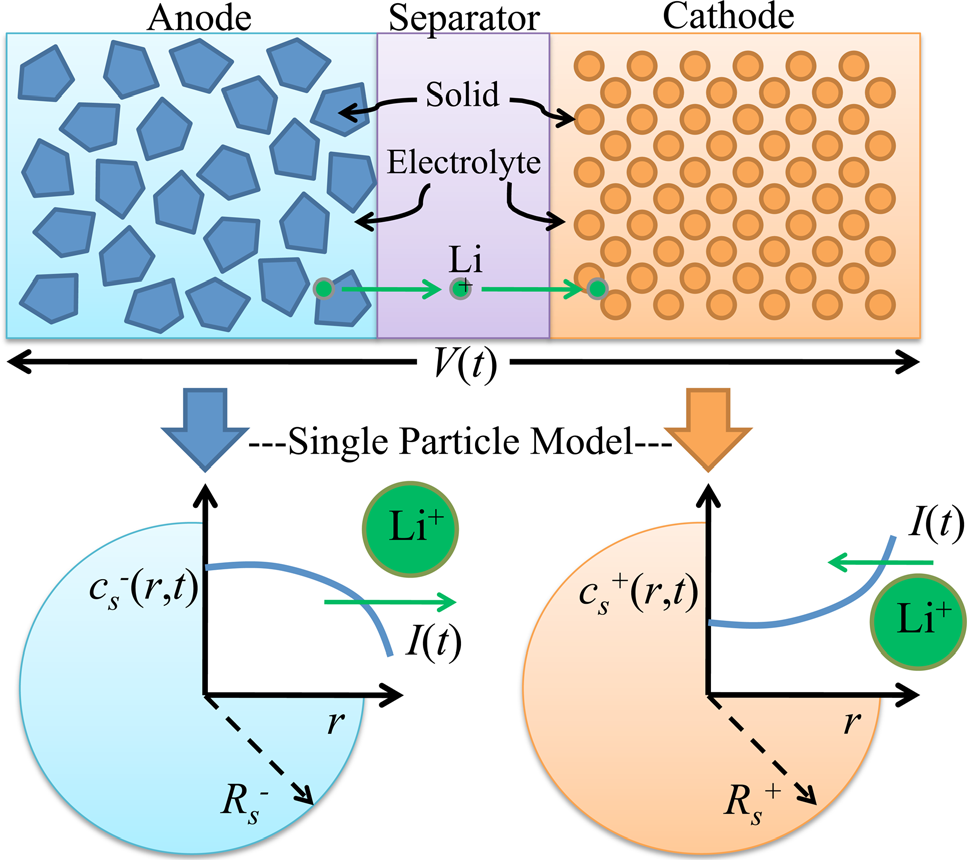
\includegraphics{spm_geometry}};
        \begin{scope}[x={(image.south east)},y={(image.north west)}]
            \node[fill=mourablue,inner sep=0pt,outer sep=0pt] at (0.265,0.045) {\scriptsize $\text{p}_\text{n}$};
            \node[minimum height=3mm, minimum width=2mm,fill=mourablue,inner sep=2pt,outer sep=2pt] at (0.27,0.09) {};
            \node[fill=mouraorange,inner sep=0pt,outer sep=0pt] at (0.785,0.045) {\scriptsize $\text{p}_\text{p}$};
            \node[minimum height=3mm, minimum width=2mm,fill=mouraorange,inner sep=2pt,outer sep=2pt] at (0.80,0.085) {};
        \end{scope}
    \end{tikzpicture}
    \caption[Schematic illustration depicting geometrical origins of the
    \glsfmtshort{spm}]
    {%
        Schematic illustration depicting the geometrical origins of the basic
        \gls{spm}. The model is obtained through a degenerate spatial
        discretisation of one electrochemical layer of a  pouch cell.  The
        active material of each porous electrode is represented by one
        representative spherical particle, thus entirely eliminating the spatial
        dimension along the axial direction. Illustration adapted
        from Moura~\etal~\cite{Moura2012}.
    }%
    \label{fig:sandwichtospm}
\end{figure}

\subsection{Scope and Assumptions}\label{subsec:basicspmassumptions}

Having described the  geometrical representation of the model,  it is imperative
to establish its  aims and scope. This section discusses  the subset of physical
phenomena  that can  be  captured  by the  basic  \gls{spm}  and enumerates  the
inherent assumptions in model derivation.  The validity of these assumptions and
their effects  on model accuracy shall  be examined in the  results presented in
\cref{subsec:simresultsbasicspm}. As  a broad  outline of  its scope,  the model
attributes the cell polarisation to two dominant physics \viz~reaction kinetics
and solid phase transport phenomena \ie~diffusion dynamics.


The  \gls{spm}  assumes that  charge  transfer  happens throughout  the  surface
of  each  representative  spherical  particle where  intercalation  occurs.  The
electronic  conductivity of  the solid  phase is  assumed to  be high  enough to
ignore the spatial distribution  of charge \ie~the local  volumetric current
density is assumed  to be uniform along the thickness  of each porous electrode.
This assumption is  motivated from early calculations by Newman and
Tobias~\cite{Newman1962} in their stand-alone  analysis of current distributions
in porous electrodes, wherein a volume-averaged molar flux was deemed sufficient
throughout  the  thickness  of  the  electrode.  This  uniform  current  density
assumption implies  that all of the  particles in the electrode  active material
are  in parallel.  Solid  phase  diffusion dynamics  within  each electrode  are
therefore solved by assuming this averaged electrochemical reaction rate. In the
simulation study  by Smith and~Wang~\cite{Smith2006},  it is reported  that soon
after  the beginning  of discharge,  solid  phase concentration  and ionic  flux
become nearly  independent of  spatial position, and  that lithium  diffusion in
solid particles may be driven by an averaged molar flux at the surface.


Based  on the  discussion thus  far, it  is clear  that the  \gls{spm} does  not
attempt to  model all  physical processes  within the  cell. In  particular, the
model assumes  instantaneous charge  transport from one  electrode to  the other
through  the  solution  phase.  This  implies  that  electrolytic  diffusion  is
sufficiently  fast  (relative to  diffusion  in  the  solid phase).  Thus,  mass
transport  phenomena  in  the  electrolyte  have been  neglected  in  the  basic
\gls{spm}.


During   the  operation   of  the   cell,   the  \gls{spm}   assumes  that   the
electrolyte  concentration~$c_\text{e}$  remains  constant  at  its  equilibrium
initial value~$c_{\text{e},0}$  throughout the cell thickness.  Neglecting local
concentration gradients in  the solution phase, together with  ignoring its mass
transport phenomena, implies  that the current in the electrolyte  does not vary
over  space  and  time.  Hence,  in  the  conventional  \gls{spm}  there  is  no
contribution of the solution phase  to internal overpotentials \ie~electrolyte
dynamics have  no influence on the  cell's terminal voltage. The  \gls{spm} also
ignores any  variations in material  porosities in each  electrode. Furthermore,
all solid phase diffusivities and kinetic parameters are held constant. Finally,
all thermal effects are assumed to  be negligible and no degradation effects are
attempted to be modelled in the basic \gls{spm} formulation.

These  simplifying  assumptions  are  made  so as  to  facilitate  the  ease  of
implementing a  \gls{pbm}, without incurring  the heavy computational  cost that
typically accompanies it. The impact of these assumptions on the accuracy of the
model shall  be examined in \cref{subsec:simresultsbasicspm}  and later sections
presents prior research that strives to  straddle the fine balance between model
sophistication and computational complexity.

\subsection{Governing  Equations}\label{subsec:basicspmgoverningeqns}
% {Governing  Equations\protect\footnote{In  this
% section,   only  those   simplifications  to   mathematical  notations   arising
% due  to  assumptions  discussed  in \cref{subsec:basicspmassumptions}  shall  be
% introduced   in-line.   For  a   comprehensive   reference   to  the   notations
% used,   please  refer   to   nomenclature   list  in   the~\nameref{ch:glossary}
% chapter.  Notations  introduced  solely  for   this  section  are  also  covered
% here.}}


As discussed  in \cref{subsec:basicspmassumptions},  the \gls{spm}  captures the
cell's dynamics arising due to diffusion  and kinetics at the two representative
spherical electrodes. It also accounts for the contribution of their equilibrium
thermodynamics to the cell's \gls{ocp}.

\subsubsection*{Solid Phase Diffusion}

Conservation of \ch{Li^0} in the electrodes can be obtained by assuming that the
movement of neutral  atoms within the solid phase is  primarily due to diffusion
within particles.  This diffusion  phenomena is induced  due to  a concentration
gradient that  exists between the surface  and interior/core of the  solid phase
particles. Based on the geometrical assumptions of the \gls{spm} as discussed in
\cref{subsec:basicspmgeometry} \ie~owing to the lack of spatial discretisation
in  the  axial  direction~$x$,  the  concentrations  of  \ch{Li^0}  in  the  two
electrodes~$c_\sj(x,r,t)$, reduce  to a  function of the  radial co-ordinate~$r$
and time~$t$, and is denoted by~$c_\sj(r,t)$,~\jinnegpos{}. To keep the notation
tractable, this  explicit spatio-temporal radial dependence  is omitted, further
simplifying the representation  to~$c_\sj$. We start with the  derivation of the
solid-phase diffusion equation \cref{eq:dfnsoliddiff} in \cref{tbl:dfneqns}, and
then proceed  to the simplifications  of its boundary conditions  facilitated by
the \gls{spm} assumptions.

Diffusion  in the  solid phase  can be  modelled by  applying classical  Fickian
dynamics~\cite{Fick1995} given by
\begin{equation}\label{eq:cartesiandiffusion}
    \diffp{c_\sj}{t} = ∇\! ⋅ \left(D_\sj\, ∇ c_\sj \right)\qquad \jinnegpos{}%\footnotemark{}
\end{equation}
% \footnotetext{For  the  sake of  brevity,  in  rest  of  the equations  in  this
% section,  the  explicit  definition  for   each  subsequent  occurrence  of  the
% subscripted variable $j$ shall be omitted. It is implied that \jinnegpos{} since
% these  equations describe  solid phase  diffusion in  the negative  and positive
% electrodes.}
The  divergence of  a vector  field~$\mathbf{F}(r,θ,ϕ)$ can  be expressed  in
spherical co-ordinates as
\begin{equation}\label{eq:fullsphericaldiv}
    ∇ ⋅ \mathbf{F} = \frac{1}{r^2}\diffp{\left(r^2 F_r\right)}{r} +
    \frac{1}{r \sin θ}\diffp{\left(\sin θ\:  F_θ\right)}{θ}
    + \frac{1}{r \sin θ}\diffp{F_ϕ}{ϕ}
\end{equation}
where  $r$~denotes the  radius,  $θ$~the polar  angle,  and $ϕ$~the  azimuthal
angle. $F_r, F_θ$ and $F_ϕ$~denote  the corresponding components of the vector
field~$\mathbf{F}$.

The  co-ordinate  origin  at  each  electrode is  aligned  with  the  centre  of
its  representative  spherical  particle.  Due  to symmetry  in  the  polar  and
azimuthal axes, the  divergence becomes a function of only  the radial position.
\Cref{eq:fullsphericaldiv} therefore reduces to
\begin{equation}\label{eq:reducedsphericaldiv}
    ∇ ⋅ \mathbf{F} = \frac{1}{r^2}\diffp{\left(r^2 F_r\right)}{r}
\end{equation}
Applying     the     \gls{rhs}     of     the     divergence     operator     of
\cref{eq:reducedsphericaldiv} in \cref{eq:cartesiandiffusion} yields
\begin{equation}\label{eq:csdiffusioneqn}
    \diffp{c_\sj}{t} = \frac{1}{r^2}\diffp*{\left(r^2 D_\sj\, ∇ c_\sj \right)}{r}
\end{equation}
As   per  the   assumption  of   uniform   diffusivity  in   the  solid   phase,
\cref{eq:csdiffusioneqn} becomes
\begin{align}
    \diffp{c_\sj}{t} &= \frac{D_\sj}{r^2}\diffp*{\left(r^2 ∇ c_\sj \right)}{r}\label{eq:csdiffusionconstdiffusivity}
    \intertext{Applying the gradient operator of \cref{eq:csdiffusionconstdiffusivity} along
    the radial direction~$r$,}
    \diffp{c_\sj}{t} &= \frac{D_\sj}{r^2}\diffp*{\left(r^2 \diffp{c_\sj}{r}
    \right)}{r}\ \text{.}\label{eq:csdiffusionfinal}
\end{align}
\Cref{eq:csdiffusionfinal} represents  a mass-balance equation  describing solid
phase diffusion  in each electrode  and is  identical to the  governing equation
\cref{eq:dfnsoliddiff} from \cref{tbl:dfneqns}. The  potential at each electrode
depends  on   the  solid  phase  surface   concentration~$c_\sjsurf$  \ie~the
\ch{Li^0}~concentration~$c_\sj(r,t)$  evaluated at~$r=R_\pj$,~\jinnegpos{} where
$R_\pj$~represents  the  equivalent  radius  of  each  representative  spherical
particle.

Due to spherical symmetry,  flux at the centre of the  particle is considered to
be zero.
\begin{equation}\label{eq:csfluxcentre}
    \diffp{c_\sj}{r}{\mathrlap{r=0}} = 0
\end{equation}
\addlines[0.5]
Diffusion in the solid phase is driven by concentration gradients induced due to
intercalation flux  density at the  particle surface  \ie~the surface  of each
particle experiences a pore-wall flux density driven by reaction kinetics. Based
on  the  \gls{spm}  geometry discussed  in  \cref{subsec:basicspmgeometry},  the
spatial dependence of this molar  flux density~$j_\nj(x,t)$ is eliminated and it
can  therefore  be  represented  as~$j_\nj(t)$,~\jinnegpos{}. For  the  sake  of
brevity,  its  explicit temporal  dependence  is  also  omitted resulting  in  a
simplified notation~$j_\nj$. Hence, at the particle surface
{%
\setlength{\abovedisplayskip}{5pt}
\begin{equation}\label{eq:csfluxsurface}
    D_\sj\diffp{c_\sj}{r}{\mathrlap{r=R_\pj}} = -j_\nj
\end{equation}
}%
The sign convention chosen here is such that pore-wall flux leaving the particle
surface is considered to be negative.

Charge   conservation   in   solid   phase    is   applied   to   evaluate   the
\gls{rhs}  in \cref{eq:csfluxsurface},   a  detailed  derivation  of   which  is
presented  in  Domenico~\etal~\cite{DiDomenico2010}.  In  summary,  by  assuming
a  uniform   charge  density   throughout  the   thickness  of   each  electrode
(see \cref{subsec:basicspmassumptions}), we get
\begin{align}
    j_\nj(t)                       &= ± \frac{I(t)}{A \, l_j a_\sj F}\label{eq:uniformcurrdensity}   \qquad \jinnegposordered
    \intertext{Substituting \cref{eq:uniformcurrdensity} in \cref{eq:csfluxsurface}}
    D_\sj\diffp{c_\sj}{r}{\mathrlap{r=R_\pj}} &= ∓ \frac{I}{A \, l_j a_\sj F}\label{eq:csfluxsurfacefinal} \qquad \jinnegposordered
\end{align}
wherein  the  load current~${I(t)  >  0}$  for discharge,  whose  explicit
time-dependence  has  been  omitted in  \cref{eq:csfluxsurfacefinal}  for  being
consistent notation with the \gls{lhs}. The positive and negative signs apply to
the negative  and positive  electrode respectively as  indicated by  the ordered
pair \jinnegposordered. It  should be noted that the term  involving the Faraday
constant in the \gls{rhs}  of \cref{eq:uniformcurrdensity} is~$nF$, where $n$~is
the number  of electrons  transferred during the  reaction. However,  since this
thesis only  discusses lithium-ion  chemistries where~$n=1$, this  is implicitly
conveyed and shall be omitted for all potential occurrences.

The cell's \gls{soc} can be obtained from the bulk concentration of lithium
in  either the  negative  or  positive electrode.  By  convention, the  negative
electrode is used.
\begin{equation}\label{eq:socinitialdefn}
    z(t) = \frac{3}{c_\snegmax}∫_0^{R_\pneg}r^2 c_{s_\text{neg}} (r,t)\, dr
\end{equation}

Given an  initial cell  \gls{soc}~${z(0) = z_0}$  at rest,  the equilibrium
concentration of \ch{Li^0} in the two individual electrodes can be computed as
\begin{equation}\label{eq:csfluxinitialcondition}
    c_\sj(r,0) = c_\sjmax \, \bigg[z_0 \left(θ_\maxj - θ_\minj \right) + θ_\minj \bigg]
\end{equation}
where $\theta_\maxj$ and $\theta_\minj$ are the electrode stoichiometries at
\SI{100}{\percent}~\gls{soc} and \SI{0}{\percent}~\gls{soc} respectively.

\Cref{eq:csdiffusionfinal},          its         corresponding          boundary
conditions~\eqref{eq:csfluxcentre} and~\eqref{eq:csfluxsurfacefinal}  along with
initial   condition~\eqref{eq:csfluxinitialcondition},   provide  the   complete
description of  time-domain evolution of  lithium in the  conventional \gls{spm}
for  a  given  applied  current  profile~$I(t)$.  Considerations  for  efficient
numerical simulation of this system is presented next.

%  in \cref{subsec:basicspmgeometry}.


\subsubsection*{Further Reduction in Dimensionality}\label{subsec:basicspmfurtherdimensionalityreduction}

A naive approach to numerically solving the solid phase diffusion equation is to
discretise each of the two representative particles in the radial direction~$r$.
Given the elaborate  simplifications made to remove spatial  resolution from the
axial  direction, the  efficacy of  using  a radial  discretisation is  rendered
questionable, particularly within the scope of  embedding the model in an online
simulation and  state-estimation environment. Since diffusion  in each spherical
particle is modelled by the well-known Fickian dynamics~\cite{Fick1995}, several
attempts have  been made to  obtain an  approximate analytical solution  for the
solid phase concentration in both electrodes.
% In  the  context  of  \gls{spm}  modelling, the  earliest  such  work \ie~a
% comparison of  the discretised version  with an approximate  analytical solution
% was performed by Santhanagopalan~\etal~\cite{Santhanagopalan2006}.
In a  dimensionless analysis study,  Zhang and White~\cite{Zhang2007}  provide a
comparative  evaluation of  the various  approximation methods  for solid  phase
diffusion, a summary of which is presented in \cref{tbl:solidphaseapprox}.

% -*- root: ../main.tex -*-
%!TEX root = ../main.tex

\begin{table}[!htbp]
    \caption[Solid phase diffusion approximation methods]{Summary of approximation methods for solid phase diffusion}
    \label{tbl:solidphaseapprox}
    \centering
    \begin{tabular}{@{}ll@{}}\toprule
        Method                     & Introduced by                                             \\ \midrule
        Duhamel's superposition    & Doyle, Fuller \&  Newman~\cite{Doyle1993,Fuller1994}      \\
        Diffusion length           & Wang~\etal~\cite{Wang1998}                                \\
        Corrected Diffusion length & Wang and Srinivasan~\cite{Wang2002}                 \\
        Polynomial approximation   & Subramanian~\etal~\cite{Subramanian2001a,Subramanian2005} \\
        Pseudo steady-state        & Liu~\cite{Liu2006}                                        \\
        \bottomrule
    \end{tabular}
\end{table}


In the  aforementioned study, the computational  burden \ie~storage requirements
and  \gls{cpu}  times  of  Duhamel's   superposition  method  was  found  to  be
excessively  high to  warrant further  interest  in it.  The original  diffusion
length method proposed  by Wang~\etal{} is valid only after  the diffusion layer
builds  up  to its  steady  state,  and hence  leads  to  significant errors  in
transient  conditions.  Although Wang  and  Srinivasan  introduced an  empirical
correction factor to  the diffusion length to extend its  validity to short-time
scale operations, this  affected the convergence of the method  for steady state
conditions.  The pseudo  steady state  solution proposed  by Liu  uses a  finite
integral  transform  technique  to  eliminate the  radial  dependence  of  solid
phase concentration.  However, this method uses  computations involving infinite
summations,  exponential  and trigonometric  quantities,  which  in this  thesis
author's view, makes it less attractive for online implementations.

The         literature         on          polynomial         methods         by
Subramanian~\etal{}~\cite{Subramanian2005} provide  detailed derivations  of the
\engordnumber{2}~and   \engordnumber{4}~order  polynomial   approximations.  The
\engordnumber{2}~order solution was found to have poor performance for transient
behaviour, similar  to that  of the original  diffusion length  method. However,
higher order polynomial  approximations were found to  provide acceptable levels
of  performance  for  both  transient  and steady  state  conditions  and  shall
therefore be examined further.

The  polynomial   approximation  method  describes  the   dynamic  evolution  of
the  volume  averaged concentration
\begin{equation}
    c_\sjavg(t)  = \frac{1}{Ω}  ∫\limits_Ω c_\sj(r,t)\,  dΩ
\end{equation}
as  a function  of the  applied load  current~$I(t)$. Here,  $Ω$~represents the
volume  of  the spherical  particle.  For  notational brevity,  $c_\sjavg(t)$~is
shortened to~$\mean{c}_\sj$ whilst also dropping its explicit time dependence.

The \engordnumber{4}~order polynomial approximation assumes that the solid phase
concentration~$c_\sj(r,t)$ is a quartic function of the radial co-ordinate~$r$.
\begin{equation}\label{eq:fourthorderpoly}
    c_\sj(r,t) = a(t) + b(t)\left(\frac{r}{R_\pj}\right)^2 + d(t) \left(\frac{r}{R_\pj}\right)^4
\end{equation}

\addlines[0.5]
The    detailed   derivation    of   the    coefficients~${a(t),    b(t)
\text{ and } c(t)}$     is     provided    in     Subramanian~\etal{}~\cite{Subramanian2005}.
\Cref{eq:csmeanevolution,eq:qmeanevolution,eq:csurffromcsavg}    summarise   the
governing equations  obtained by applying the  \engordnumber{4}~order polynomial
approximation of \cref{eq:fourthorderpoly}  to the system of  equations given by
\cref{eq:csdiffusionfinal,eq:csfluxcentre,eq:csfluxsurfacefinal}.
\begingroup
\allowdisplaybreaks
\setlength{\abovedisplayskip}{5pt}
\begin{align}
    \diff*{\mean{c}_\sj}{t} + 3\frac{j_\nj}{R_\pj}                                                &=0 \label{eq:csmeanevolution} \\
    \diff*{\mean{q}_j}{t} + 30\frac{D_\sj}{R_\pj^2}\mean{q}_j + \frac{45}{2}\frac{j_\nj}{R_\pj^2} &=0 \label{eq:qmeanevolution}\\
    35\frac{D_\sj}{R_\pj}\left(c_\sjsurf - \mean{c}_\sj\right) - 8D_\sj \mean{q}_j                &= -j_\nj \label{eq:csurffromcsavg}
\end{align}%
\endgroup
where $\mean{q}_j(t)$~represents  the volume  averaged concentration  flux, that
defines  the  average  change  of  concentration  with  respect  to  the  radial
position~$r$.

As   per  \cref{eq:uniformcurrdensity},   the   interfacial   flux  density   is
proportional to  the applied current. Hence  \cref{eq:csmeanevolution} implies a
simple linear relationship between the applied current and the rate of evolution
of average \ch{Li^0}~concentration within  each spherical particle. This further
implies  that the  \gls{soc} of  the cell  has a  linear rate-dependence  on the
externally  applied  current. Furthermore,  due  to  the elimination  of  radial
discretisation, the computation of \gls{soc}, given by \cref{eq:socinitialdefn},
reduces to the task of first computing the ratio of bulk (average) concentration
to  surface concentration  and  then adjusting  it to  account  for the  useable
stoichiometry limits for the relevant electrode. Thus, the cell's \gls{soc}
% as predicted by the \gls{spm}
can be computed as
\begin{equation}\label{eq:soccomputation}
    z = \frac{\tfrac{\mean{c}_\sneg}{c_\snegmax} - θ_\minneg}{θ_\maxneg - θ_\minneg}
\end{equation}
where $\mean{c}_\sneg$~is obtained by  solving \cref{eq:csmeanevolution} for the
negative electrode.

In   the  views   of   this  author,   this  \engordnumber{4}~order   polynomial
approximation   proposed  by   Subramanian~\etal~\cite{Subramanian2005}  strikes
an  acceptable  balance  between   the  three  modelling  pivots ---
\begin{enumerate*}[label=\roman*)]
    \item computational complexity,
    \item mathematical  tractability, and
    \item numerical accuracy
\end{enumerate*}
and has therefore  been adopted for all \gls{spm} simulations  presented in this
work.

At   the   end   of    this   dimension-reduction   step,   spatial   dependence
is   completely  eliminated,   yielding   a  zero-order   (in  space)   physical
model    whose    dynamics   are    described    by    the   \gls{dae}    system
of \cref{eq:csmeanevolution,eq:qmeanevolution,eq:csurffromcsavg}.

\subsubsection*{Equilibrium Thermodynamics}\label{subsec:basicspmthermodynamics}

The equilibrium potential of a porous electrode is a thermodynamic property that
depends on the extent of lithiation in the outermost interstitial sites near the
\gls{sei} layer. This surface stoichiometry~$θ_j$  for an electrode is obtained
by  computing the  surface  concentration  (using \cref{eq:csurffromcsavg})  and
dividing by the maximum lithiation capacity of that electrode.
\begin{equation}
    θ_j = \frac{c_\sjsurf}{c_\sjmax}
\end{equation}

Although based upon the theoretical foundation  laid out by the Nernst equation,
owing  to a  multitude of  complex phase  transitions, the  potential of  porous
electrodes  (with respect  to metallic  lithium) is  usually given  as empirical
functions of its surface stoichiometry~\cite{Reddy2011,Rahn2013}.
\begin{equation}\label{eq:ocpstoichiometry}
    U_j(t) = \mathcal{U}_j\left(θ_j(t)\right)
\end{equation}
where  the  empirical  relationships~$\mathcal{U}_j$ are  typically  high  order
polynomials  or rational  functions  that  are fitted  to  relaxation data  from
\gls{gitt} experiments on half-cells~\cite{Birkl2015a,Ecker2015}.

In the \gls{spm},  the cell's \gls{ocp} is obtained by  subtracting the negative
electrode  equilibrium  potential~$U_\text{neg}$  from  its  positive  electrode
counterpart~$U_\text{pos}$, as shown in \cref{eq:ocpdefinition}.
\begin{equation}\label{eq:ocpdefinition}
    U_\text{ocp} = U_\text{pos} - U_\text{neg}
\end{equation}
Even though the  concept of \gls{ocp} is defined only  in equilibrium conditions
when no  current flows,  the individual electrode  potentials themselves  form a
significant component of the cell's terminal voltage~$V(t)$.

\subsubsection*{Reaction Kinetics}

In the \gls{spm}, the reaction kinetics in each spherical electrode is modelled
using the Butler-Volmer expression (see \cref{eq:butlervolmer}).
\begin{align}
    j_\nj   &= j_{0_j} \left[ \exp\left( \frac{\left(1-α\right) F η_j}{R T}\right) -  \exp\left( \frac{-α F η_j}{R T}\right)\right] \label{eq:bvwithalpha} \\
    \shortintertext{where}
    j_{0_j} &= k_\jr c_\text{e}^{1-α} c_\sjsurf^{α} \left(c_\sjmax - c_\sjsurf\right)^{1-α}
\end{align}

The equilibrium  rate of forward  and backward  reactions at both  electrodes is
assumed  to  be  equal.  With charge  transfer  coefficient~${α  =  0.5}$,
\cref{eq:bvwithalpha} simplifies to
\begin{equation}\label{eq:BVwithalphahalf}
    j_\nj = 2 k_\jr \sqrt{c_\text{e} c_\sjsurf \left(c_\sjmax - c_\sjsurf\right)} \sinh\left(\frac{F η_j}{2 R T}\right)
\end{equation}

The  expression   for  overpotential~$η_j$   for the basic \gls{spm} can  be   obtained  by rearranging 
\cref{eq:BVwithalphahalf},     substituting    for     $j_\nj$~from by
\cref{eq:uniformcurrdensity} whilst using the initial electrolyte concentration
$c_\text{e,0}$ and is given by
\begin{equation}\label{eq:overpotential_j}
    η_j(t) =  \frac{2 R T}{F }\sinh^{-1} \left( \frac{± I(t)}{2 A \, l_j a_\sj F
    k_\jr \sqrt{c_\text{e,0} c_\sjsurf \left(c_\sjmax - c_\sjsurf\right)}}\right)
\end{equation}

\subsubsection*{Cell Terminal Voltage}\label{subsec:basicspmcellterminalvoltage}

The terminal voltage  of the cell under applied load  is obtained by subtracting
the potential of the negative electrode from its positive counterpart.

Starting from the definition of the overpotential of each electrode
\begin{align}
    η_\text{pos} &= ϕ_\spos - \cancelto{0}{ϕ_\epos} - U_\text{pos} \label{eq:posoverpotential} \\
    η_\text{neg} &= ϕ_\sneg - \cancelto{0}{ϕ_\eneg} - U_\text{neg} \label{eq:negoverpotential}
\end{align}
Within  each electrode  domain,  the contribution  of  electrolyte potential  is
neglected  (see \cref{subsec:basicspmgeometry,subsec:basicspmassumptions}  for a
brief discussion on the exclusion of electrolyte dynamics).

Subtracting \cref{eq:negoverpotential}   from \cref{eq:posoverpotential},
% whilst substituting for $U_j$ from \cref{eq:ocpstoichiometry}
\begin{align}
    η_\text{pos} - η_\text{neg} &= \underbrace{ϕ_\spos - ϕ_\sneg}_{V_\text{cell}} - U_\text{pos} + U_\text{neg}\label{eq:overpotentialdifference}\\
\shortintertext{whose rearrangement yields}
    V_\text{cell}               &= η_\text{pos} - η_\text{neg} + U_\text{pos} - U_\text{neg}\label{eq:cellterminalvoltagebasic}
\end{align}
% \mathcal{U}_\text{pos}\left(θ_\text{pos}\right) - \mathcal{U}_\text{neg}\left(θ_\text{neg}\right)
In the  basic \gls{spm},  \cref{eq:cellterminalvoltagebasic} is used  to compute
the cell's terminal voltage under  load. Although their explicit time-dependence
notation  is omitted  in  the notation  here,  it is  worth  reminding that  all
quantities in \cref{eq:cellterminalvoltagebasic} are indeed continuous functions
of time.

\subsubsection*{State Space Representation}\label{subsec:basicspmstatespace}

For control  oriented applications, it is  imperative to have a  classical state
space representation  that collates  all intermediate equations  and definitions
presented  thus  far into  a  single  system  of  equations that  describes  the
evolution of solid concentration and terminal  voltage over time, expressed as a
response to the  external current input~$I(t)$. However,  the non-linearities in
the equation for terminal voltage \ie~\cref{eq:cellterminalvoltagebasic} imply
that it is  not possible to represent  the \gls{spm} in the form  of a classical
\gls{lti}  system  of \cref{eq:LTIstatespace}.  Instead,  the  \gls{spm} can  be
summarised  by a  system  of linear  state equations  together  with the  single
non-linear output equation.

Rearranging  \cref{eq:qmeanevolution,eq:csurffromcsavg}, the  state equation  is
obtained as
\begin{equation}\label{eq:fourstatesmatrixvec}
    \setstackgap{L}{1.5\baselineskip}
    \fixTABwidth{T}
    \diff*{\parenMatrixstack{
            \vphantom{\frac{45}{2} \frac{1}{R_\ppos^2 A \, l_\text{pos} a_\spos F}}
            \mean{q}_\text{pos} \\
            \vphantom{\frac{45}{2} \frac{1}{R_\ppos^2 A \, l_\text{pos} a_\spos F}}
            % \vphantom{\frac{D_\sneg}{R_\pneg^2}}
            \mean{q}_\text{neg} \\
            \vphantom{\frac{45}{2} \frac{1}{R_\ppos^2 A \, l_\text{pos} a_\spos F}}
            % \vphantom{\frac{D_\spos}{R_\ppos^2}}
            \mean{c}_\spos \\
            \vphantom{\frac{45}{2} \frac{1}{R_\ppos^2 A \, l_\text{pos} a_\spos F}}
            % \vphantom{\frac{D_\sneg}{R_\pneg^2}}
            \mean{c}_\sneg
        }
    }{t}
    = \underbrace{\parenMatrixstack{
            -30\frac{D_\spos}{R_\ppos^2} & 0                            & 0 & 0 \\
            0                            & -30\frac{D_\sneg}{R_\pneg^2} & 0 & 0 \\
            \vphantom{\frac{45}{2} \frac{1}{R_\ppos^2 A \, l_\text{pos} a_\spos F}}
            0                            & 0                            & 0 & 0 \\
            \vphantom{\frac{45}{2} \frac{1}{R_\ppos^2 A \, l_\text{pos} a_\spos F}}
            0                            & 0                            & 0 & 0
    }}_{A}
    \parenMatrixstack{
        \vphantom{\frac{D_\spos}{R_\ppos^2}}
        \mean{q}_\text{pos} \\
        \vphantom{\frac{D_\sneg}{R_\pneg^2}}
        \mean{q}_\text{neg} \\
        \vphantom{\frac{D_\spos}{R_\ppos^2}}
        \mean{c}_\spos \\
        \vphantom{\frac{D_\sneg}{R_\pneg^2}}
        \mean{c}_\sneg
    }
    +
    \underbrace{\parenMatrixstack{
            \frac{45}{2} \frac{\hphantom{-}1}{R_\ppos^2 A \, l_\text{pos} a_\spos F} \\
            \frac{45}{2} \frac{-1}{R_\pneg^2 A \, l_\text{neg} a_\sneg F} \\
            \hphantom{\frac{45}{2}} \frac{\hphantom{-}3}{R_\ppos  A \, l_\text{pos} a_\spos F} \\
            \hphantom{\frac{45}{2}} \frac{-3}{R_\pneg  A \, l_\text{neg} a_\sneg F}
    }}_{B}
    I(t)
\end{equation}
which corresponds to the classical \gls{lti} form
\begin{equation}
    \dot{\mathbf{x}} = A\,\mathbf{x} + B\,\mathbf{u}
\end{equation}
where~${\mathbf{x}   =    \vect{\mean{q}_\text{pos},\mean{q}_\text{neg},
\mean{c}_\spos,  \mean{c}_\sneg},   \,  x  ∈  \mathbb{R}^{4   \times  1}}$  is
the  state  vector.  The  scalar system  input~$\mathbf{u}  ∈  \mathbb{R}$  is
the  applied  current~$I(t)$.  The  system matrix~${A  ∈  \mathbb{R}^{4  \times
4}}$  and  input  matrix~$B  ∈  \mathbb{R}^{4 \times  1}$  are  also  shown  in
\cref{eq:fourstatesmatrixvec}.

For state estimation and controller design purposes, it is important to keep the
number  of elements  in the  state vector  as small  as possible  by eliminating
redundant  variables.  For  instance,  Di~Dominico~\etal{}~\cite{DiDomenico2010}
noted that with  output voltage as the only measured  quantity, the observability
of   the  four-state   model  of   \cref{eq:fourstatesmatrixvec}  is   adversely
affected.  To tackle  this issue,  a  state-reduction approach  was proposed  by
Di~Domenico~\etal~\cite{DiDomenico2010},  which  hinges  upon the  principle  of
material balance.

The total number of moles of lithium in the system is given by
\begin{equation}\label{eq:totallithiummoles}
    n_\text{Li} = \frac{ε_\spos \, l_\text{pos}\, A}{\frac{4}{3} π R_\ppos^3} ∫_0^{R_\ppos} 4 π r^2 c_\spos(r,t) \, dr
    +  \frac{ε_\sneg \, l_\text{neg}\, A}{\frac{4}{3} π R_\pneg^3} ∫_0^{R_\pneg} 4 π r^2 c_\sneg(r,t) \, dr
\end{equation}
Upon considering only the bulk concentration as per the dimensionality reduction
procedure    outlined   in \cref{subsec:basicspmfurtherdimensionalityreduction},
\cref{eq:totallithiummoles} reduces to
\begin{align}\label{eq:totallithiumsimplified}
    n_\text{Li}  &= \frac{ε_\spos \, l_\text{pos}\, A}{\frac{4}{3} π R_\ppos^3}\mean{c}_\spos ∫_0^{R_\ppos} 4 π r^2  \, dr
    + \frac{ε_\sneg \, l_\text{neg}\, A}{\frac{4}{3} π R_\pneg^3}\mean{c}_\sneg ∫_0^{R_\pneg} 4 π r^2  \, dr
                \\
                 &= ε_\spos \, l_\text{pos}\, A \, \mean{c}_\spos + ε_\sneg \, l_\text{neg}\, A \, \mean{c}_\sneg
\end{align}
Assuming    no    loss   of    cycleable    lithium    or   other    degradation
mechanisms,  the   total  number  of   moles  of   lithium  in  the   system  is
conserved   \ie~${\diff{n_\text{Li}}{t}   =  0}$.   Substituting   this   into
\cref{eq:totallithiumsimplified},
\begin{align}
    0                          &= \phantom{+} \diff*{ε_\spos \, l_\text{pos}\, A \, \mean{c}_\spos }{t} + \diff*{ε_\sneg \, l_\text{neg}\, A \, \mean{c}_\sneg }{t} \\
    \diff*{\mean{c}_\spos}{t}  &= -\diff*{\mean{c}_\sneg}{t} \label{eq:bulkconcrelationship}
\end{align}

As  per   \cref{eq:bulkconcrelationship},  the   time  evolution  of   the  bulk
concentration  of one  electrode can  be obtained  as a  function of  the other.
Furthermore, Di~Domenico~\etal{}~\cite{DiDomenico2010}  show that  the diffusion
dynamics of the  bulk concentrations can be algebraically  related through their
stoichiometric factors as
\begin{equation}\label{eq:csposbulkfromcsnegbulk}
    \mean{c}_\spos(t) = c_\sposmax \, \left[\frac{\mean{c}_\sneg(t)- θ_\minneg
    c_\snegmax}{\left(θ_\maxneg - θ_\minneg\right)c_\snegmax} \left(θ_\maxpos - θ_\minpos \right) + θ_\minpos \right]
\end{equation}

Hence, it  is possible  to eliminate the  bulk concentration of  any one  of the
electrodes from the state-equation to arrive at a three-state description of the
model dynamics. In  extant lithium-ion chemistries, owing to  its proclivity for
lithium deposition during  charging, the negative electrode is  considered to be
the limiting electrode (See  Arora~\etal~\cite{Arora1999}). Hence it is retained
in the state vector, thereby leading to  the final form of the state dynamics of
the conventional \gls{spm} as
\begin{equation}\label{eq:threestatesmatrixvec}
    \setstackgap{L}{1.5\baselineskip}
    \fixTABwidth{T}
    \diff*{\parenMatrixstack{
            \vphantom{\frac{45}{2} \frac{1}{R_\ppos^2 A \, l_\text{pos} a_\spos F}}
            \mean{q}_\text{pos} \\
            \vphantom{\frac{45}{2} \frac{1}{R_\ppos^2 A \, l_\text{pos} a_\spos F}}
            \mean{q}_\text{neg} \\
            \vphantom{\frac{45}{2} \frac{1}{R_\ppos^2 A \, l_\text{pos} a_\spos F}}
            \mean{c}_\sneg
        }
    }{t}
    = \underbrace{\parenMatrixstack{
            -30\frac{D_\spos}{R_\ppos^2} & 0                            & 0  \\
            0                            & -30\frac{D_\sneg}{R_\pneg^2} & 0  \\
            \vphantom{\frac{45}{2} \frac{1}{R_\ppos^2 A \, l_\text{pos} a_\spos F}}
            0                            & 0                            & 0
    }}_{A}
    \parenMatrixstack{
        \vphantom{\frac{D_\spos}{R_\ppos^2}}
        \mean{q}_\text{pos} \\
        \vphantom{\frac{D_\sneg}{R_\pneg^2}}
        \mean{q}_\text{neg} \\
        \vphantom{\frac{D_\spos}{R_\ppos^2}}
        \mean{c}_\sneg
    }
    +
    \underbrace{\parenMatrixstack{
            \frac{45}{2} \frac{\hphantom{-}1}{R_\ppos^2 A \, l_\text{pos} a_\spos F} \\
            \frac{45}{2} \frac{-1}{R_\pneg^2 A \, l_\text{neg} a_\sneg F} \\
            \hphantom{\frac{45}{2}} \frac{-3}{R_\pneg  A \, l_\text{neg} a_\sneg F}
    }}_{B}
    I(t)
\end{equation}

The  measured   variable~${y  ∈  \mathbb{R}}$  is   the  cell's  terminal
voltage~$V(t)$ and  is expressed as  a non-linear  scalar function of  the state
vector and the load current.
\begin{equation}\label{eq:spmoutputeqn}
    y = h\left(\mathbf{x}(t),u(t)\right)
\end{equation}
The output  equation given by \cref{eq:spmoutputeqn} includes  a non-zero direct
feedthrough dependency  of the voltage  on the input current,  thereby modelling
the resistive component of the cell's  impedance. The full expression for output
voltage is given by expanding \cref{eq:cellterminalvoltagebasic} as
\begin{multline}
    V_\text{cell}(t) = \frac{2 R T}{F }\sinh^{-1} \left( \frac{- I(t)}{2 A
    l_\text{pos} a_\spos F k_\posr \sqrt{c_\text{e,0} c_\spossurf(t)
    \left(c_\sposmax - c_\spossurf(t)\right)}}\right) \\
    - \frac{2 R T}{F }\sinh^{-1} \left( \frac{I(t)}{2 A \, l_\text{neg} a_\sneg F
    k_\negr \sqrt{c_\text{e,0} c_\snegsurf(t) \left(c_\snegmax - c_\snegsurf(t)\right)}}\right) \\
    + \mathcal{U}_\text{pos}\left(c_\spossurf(t)\right) -
    \mathcal{U}_\text{neg}\left(c_\snegsurf(t)\right)\label{eq:spmbasicoutputvoltagefinal}
\end{multline}
wherein the solid  phase surface concentration at  each electrode~$c_\sjsurf$ is
obtained  from its  corresponding bulk  concentration~$c_\sjavg$ by  rearranging
\cref{eq:csurffromcsavg} and is given by
\begin{align}
    c_\spossurf &= \mean{c}_\spos  + \frac{8R_\ppos}{35} \mean{q}_\text{pos}
    +\frac{R_\ppos}{35 D_\spos A \, l_\text{pos} a_\spos F} I(t)
    \label{eq:csurfposfromcavgpos}\\
    c_\snegsurf &= \mean{c}_\sneg  + \frac{8R_\pneg}{35} \mean{q}_\text{neg} -\frac{R_\pneg}{35 D_\sneg A \, l_\text{neg} a_\sneg F} I(t)\label{eq:csurfnegfromcavgneg}
\end{align}
where~${I(t) > 0}$ for discharge.

Given the initial  \gls{soc} of the cell~$z(0)$, the  initial bulk concentration
of   the  negative   electrode  at   equilibrium~$c_\sneg(0)$  is   obtained  by
\cref{eq:csfluxinitialcondition}.  The   initial  value   of  the   mean  radial
concentration flux  in both  electrodes is zero  \ie~${q_j(0) =  0}$. Therefore,
the  initial  state  vector  is~$\vect{0,0,c_\sneg(0)}$.  Thus,  the  system  of
equations given by \crefrange{eq:csposbulkfromcsnegbulk}{eq:csurfnegfromcavgneg}
form a complete  state-space representation of the  conventional \gls{spm}. This
state-space model  can be  simulated as  a standalone  \gls{ivp} or  embedded as
the  plant model  in control-oriented  applications  such as  for dynamic  state
estimation.


% % \needspace{1\baselineskip}
% \section{Numerical Implementation}\label{sec:numericalimplementation}
% % -*- root: ../../main.tex -*-
%!TEX root = ../../main.tex
% this file is called up by main.tex
% content in this file will be fed into the main document
% vim:textwidth=80 fo=cqt

The  equations  presented   in  \cref{sec:spmmodeldevelopment}  are  well-known,
self-sufficient and  fully descriptive so  as to implement the  basic \gls{spm}.
Although discrete-time numerical implementation  of circuit-oriented cell models
have been considered~\cite{Plett2004,Plett2004a,Plett2004b,Plett2006}, there has
been  no such  treatment  of this  critical aspect  in  the \gls{spm}  modelling
literature. Since  this thesis has  a strong focus  towards enabling the  use of
physics-based models in an embedded  environment, at least the numerical aspects
of implementing  these equations  need to  be discussed.  The finer  details and
practical engineering considerations of real-time programming, in particular the
integration of  the cell model into  the pack and its  interaction with upstream
components and other  such aspects of a typical  vehicular drivetrain controller
is beyond  the scope of  this academic  work. Nevertheless, the  discussion here
aims  to  lower  the  barrier  to  real-time  implementation  and  is  a  unique
contribution in the context of the cell modelling art.

\subsection{Continuous-time Implementation}
\subsubsection*{Analytical solution}
Although  not   explicitly  given  in  \gls{spm}   literature,  using  \gls{lti}
system  theory,  the  analytical  solution for  continuous-time  state  equation
(\cref{eq:LTIstatespace})  with  current input\footnote{Analytical  closed  form
solution  cannot be  obtained for  constant voltage  operation. This  is because
the  boundary flux  is  implicitly determined  by  the non-linear  Butler-Volmer
equation \cref{eq:butlervolmer}  and needs  to be  solved numerically  with some
variant of a Newton-type iteration scheme.} is given by
\begingroup
\allowdisplaybreaks
% \setlength{\abovedisplayskip}{0.9765625ex}
% \setlength{\abovedisplayskip}{0.1765625ex}
% \setlength{\belowdisplayskip}{0ex}
\begin{align}
    % \SwapAboveDisplaySkip
    \mathbf{x}(t) &= e^{A (t-t_0)}\mathbf{x}(t_0) + \int_{t_0}^{t}e^{A (t-τ)}B \mathbf{u}(τ)\,dτ \label{eq:genanalyticctssoln}
    \\
    \shortintertext{With a standard \gls{ivp}, $t_0 = 0$}
    \mathbf{x}(t) &= e^{A t}\mathbf{x}(0) + \underbrace{\int_{0}^{t}e^{A (t-τ)}B \mathbf{u}(τ)\,dτ}_{\text{convolution integral}}\label{eq:analyticalctssoln}
\end{align}
\endgroup

The matrix exponential $e^{At}$ is known as the state-transition matrix and is
defined as
\begin{equation}
    e^{A t} ≜ \mathcal{L}^{-1}\left\{(s I - A)^{-1}\right\}
\end{equation}
although several methods exist for its efficient numeric
computation~\cite{Moler2003}.

The analytical solution  given by \cref{eq:analyticalctssoln} can  be applied to
obtain the  matrix-vector state  equation \cref{eq:threestatesmatrixvec}  of the
\gls{spm}.  Once the  state  variables  are obtained  for  any time-step,  after
evaluating the  surface concentrations as per  \cref{eq:csurfposfromcavgpos} and
\cref{eq:csurfnegfromcavgneg}, the resulting values  may be substituted into the
output  equation of  \cref{eq:spmbasicoutputvoltagefinal} to  obtain the  cell's
terminal voltage.

\subsubsection*{Numerical considerations for continuous time implementation}

The procedure described  thus far has a practical limitation.  The input current
$I(t)$  to the  cell has  been defined  as a  continuous quantity.  Although for
the  purpose of  characterising  the cell's  behaviour, it  is  possible to  use
pre-determined continuous-functions as load profiles (\eg{}~sinusoidal waveforms
for virtual \gls{eis} testing), it is desirable to evaluate the model's response
to typical real-life conditions. In a vehicular application, only the samples of
cell current measured by sensors at  discrete-time intervals are reported to the
\gls{bms}. A \gls{zoh} operation is used at the model's input \ie~the level of
current  is assumed  to be  held constant  between two  successive measurements.
% Current profiles can be computed from standard drive cycle data.

It    is    tedious    to    hand-compute   the    convolution    integral    of
\cref{eq:analyticalctssoln}.   However,  a   variety   of  state   of  the   art
adaptive-time  solvers  employing  numerical  schemes  such  as  Dormand-Prince,
Runge-Kutta,  Collocation and  Backward  Differentiation  Formula are  available
to  efficiently  handle  such  \glspl{ode}. Given  that  lithium  concentrations
vary smoothly  over time  without abrupt  discontinuities, a  standard non-stiff
solver  of  moderate   order  shall  suffice.  A  single  line   of  code  using
\textsc{MATLAB}'s ode45  solver can  implement this  time integration,  \eg{} \\
\mintinline{matlab}{[~,x_new] =  ode45(@(t,x) stateEqn(x,Ik,spm_params), t_span,
x_old); }

Since  the direction  of applied  current  is susceptible  to sudden  reversals,
(\eg{}  due to  acceleration and  braking events  for a  vehicular application),
the  solver   needs  to   be  stopped  and   re-started  every   sample  period.
\Cref{alg:ctstimespm} shows the  sequence of operations in  a desktop simulation
of  the  continuous time  \gls{spm}  on  a  digital  computer. The  source  code
listing  of  an  example  implementation   in  \textsc{MATLAB}  is  provided  in
\cref{sc:ctstimespm}.
% \vspace{3ex}
% -*- root: ../main.tex -*-
%!TEX root = ../main.tex
% this file is called up by main.tex
% content in this file will be fed into the main document
% vim:nospell

\begin{algorithm}[!htbp]
    \caption{Continuous-time \glsfmtshort{spm}}\label{alg:ctstimespm}
    \begin{algorithmic}[1]
        \Require Load profile \Comment{\eg{} a \texttt{csv} file of $t$ vs. C-rate}
        \Require \gls{spm} parameter set  \Comment{\eg{} stored in a struct \texttt{params}}
        \Userdata $z[1], t_\text{f,user}$, $t_\text{f,condition}$, cell capacity $I_\text{1C}$, sample rate $T_s$ \Comment{$t_\text{f,condition} \in  \left\{\texttt{max}, \texttt{min}\right\}$}
        \Ensure  $z[1], V_\text{cell}[1]$ within limits \Comment{index $[k=1] \wedgeq \text{time } (t=0) $}
        \Procedure{Simulate\gls{spm}}{}%{$z[1],t_\text{f,desired},T_s,I_\text{1C},\texttt{params}$}
            \State {$t_\text{f,desired} =
                \begin{cases}
                   \max(t_\text{f,user},t_\text{f,profile}),
                        &\text{%\scriptsize
                    if $t_\text{f,condition}$ == \texttt{max};}\\
                    \min(t_\text{f,user},t_\text{f,profile}),
                    &\text{%\scriptsize
                otherwise.}
                \end{cases}$} \Comment{\parbox[t]{0.25\textwidth}{may terminate early due to cut-off violations}}
                    \FullComment{\scriptsize Flexible end time. Extrapolate last C-rate from profile until $t_\text{f,desired}$ if necessary.}
            \State $N_\text{max} \gets \ceil*{\frac{t_\text{f,desired}}{Ts}} + 1$ \Comment{max iterations assuming no cut-offs}
            \State Allocate storage of size $\mathbb{R}^{N_\text{max}\times 1}$ for each simulation variable
            \State Compute $\mean{c}_\sneg$[1] as per \cref{eq:csfluxinitialcondition}
            \State $I[1] \gets I_\text{1C} \times  \text{C-rate}[1], \quad \mathbf{x}[1] \gets \vect{0,0, \mean{c}_\sneg[1]}$ \Comment{ $\text{C-rate}[1]$ from profile}
            \State $V_\text{cell}[1] \gets \textsc{ComputeCellVoltage}(\textbf{x}[1],I[1],\texttt{params})$ \Comment{from direct feedthrough}
            \For{$k \gets 2 : N_\text{max}$}
                \State $I[k] \gets $ interpolate from profile using \gls{zoh}
                \State Solve continuous-time equation \cref{eq:threestatesmatrixvec} \Comment{solver IC set to $x[k-1]$}
                \State $\mathbf{x}[k] \gets $ last time-entry  vector of soln.\  matrix \Comment{from an adaptive solver \eg{} \textsc{MATLAB}'s \texttt{ode45}}
                \State Compute $z[k]$ as per \cref{eq:soccomputation}
                \State $V_\text{cell} \gets \textsc{ComputeCellVoltage}(\textbf{x}[k],I[k],\texttt{param}) $
                \If {$z[k] \text{ or } V_\text{cell}[k]$ exceeded cut-off limits}
                    \State $k \gets k - 1$ \Comment{data from last  step is invalid}
                    \State \textit{break};
                \EndIf
            \EndFor
        \EndProcedure

        \OutputEqn{\textbf{x}, I, \texttt{params}}
            \State Compute $c_\snegsurf$ as per \cref{eq:csurfnegfromcavgneg}
            \Comment{consider saturating \ie{} $c_\snegmin \le c_\snegsurf \le
            c_\snegmax$}
            \State Compute $\mean{c}_\spos$ as per \cref{eq:csposbulkfromcsnegbulk}
            \State Compute $c_\spossurf$ as per \cref{eq:csurfposfromcavgpos}
            \State Compute $V_\text{cell}$ as per \cref{eq:spmbasicoutputvoltagefinal}
        \EndOutputEqn%
    \end{algorithmic}
\end{algorithm}


In  the author's  view,  the  continuous time  \gls{spm}  algorithm has  limited
practical  use.  Computing  the  convolution  integral  or  deploying  \gls{ode}
solver code  in a  microcontroller is challenging  and introduces  a substantial
computational burden. Although the continuous time model can be used for desktop
simulation, more sophisticated \glspl{pbm} are  already available for this task.
Therefore,  for online  deployment  in  state estimation  and  control tasks,  a
discrete-time  version of  the model  suitable for  real-time implementation  is
needed.

% Nevertheless,  the  continuous time  \gls{spm}  has  one important  application,
% \viz{} estimation of physical parameters.
% which will  explored  in \cref{sec:spmparameterestim}.

\subsection{Conceptual Overview of Real-Time Processing}

The equations  in \cref{sec:spmmodeldevelopment} are derived  in continuous time
form. In particular, the  state equation given by \cref{eq:threestatesmatrixvec}
describes  the  continuous   time  dynamic  evolution  of   quantities  such  as
the  bulk  concentration and  rate  of  mean  radial  flux. However,  a  typical
embedded  controller such  as that  used in  a vehicular  \gls{bms} operates  in
discrete-time~\cite{Andrea2010}.  This implies  that \emph{samples}  of voltage,
current  and   temperature  measurements  are   obtained  at  a   periodic  time
interval~$T_s$. The  updating of  solution variables  are performed  between two
successive data acquisition events from the sensors.

% The  computations of  the  model  equations and  updates  of solution  variables
% (such as  bulk concentrations  and terminal voltage)  are performed  between two
% successive data acquisition events from the sensors.


Control-oriented  reduced-order  \glspl{pbm} such  as  the  \gls{spm} and  their
associated computations are modular elements  of a vehicular \gls{bms}. A single
\gls{bms}  often provides  a whole  host of  other auxiliary  functionality such
as  cell balancing,  protection, diagnostics  and data-logging~\cite{Plett2016}.
Although  thermal   management  tasks  are  typically   delegated  to  dedicated
controllers, the \gls{bms} software routines often handle data exchanged between
various  controllers on  the vehicular  communication bus.  While some  of these
tasks such  as book-keeping and  diagnostics can be done  at a low  rate, others
such as those  involving measurements from cell  and model-related computations,
need to be performed with high priority.

\begin{figure}[!tbp]
    \savebox{\algboxA}{%
        \begin{varwidth}[b]{0.65\linewidth}
            \begin{flushleft}
                \vspace*{1.5ex}
                \begin{algorithmic}[0]

                    \Initialise \gls{soc} \& other global variables
                    \Ensure voltage, current \& temperature limits
                    \Procedure{Main}{$ $}

                    \State configure interrupts
                    \State enable timers
                    \State $\vdots$
                    \While{\textproc{True}} \Comment[\scriptsize]{until ``key off" or shutdown}
                    \State background task \#1 \Comment[\scriptsize]{diagnostics/protection}
                    \State background task \#2 \Comment[\scriptsize]{\textproc{canbus} communication}
                    \State $\vdots$
                    \If{\texttt{needs\textunderscore balancing == 1}}
                    \Function{PackBalance}{$n_\text{cells}$,$\text{\gls{soc}}_i$,$v_i$}
                    \State \textit{subroutine for pack balancing}
                    \State $\vdots$
                    \EndFunction
                    \EndIf
                    \State $\vdots$
                    \State background task \#$n$ \Comment[\scriptsize]{supervisory reporting}
                    \EndWhile
                    \EndProcedure
                \end{algorithmic}
            \end{flushleft}%
        \end{varwidth}%
    }%
    \savebox{\algboxB}{%
        \begin{varwidth}[b]{0.65\linewidth}
            \begin{flushright}
                \vspace*{2em}
                \begin{algorithmic}[0]
                    \ISR[]{}
                    \State read new sensor data from ADC
                    \Function{ComputeSPM}{$i_{k-1}$, params}
                    \State evaluate spm model equations
                    \State $\vdots$
                    \State compute model output voltage
                    \Function{SOCEstimator}{$v_\text{model}$,$v_\text{meas}$}
                    \State \textit{state estimation subroutine}
                    \State $\vdots$
                    \EndFunction
                    \Function{ICEControl}{$ $}
                    \State $\vdots$
                    \State write control outputs to DACs
                    \EndFunction
                    \EndFunction
                    \END
                \end{algorithmic}
            \end{flushright}
        \end{varwidth}%
    }
    \centering
    \framebox[\textwidth]{
        \begin{subfigure}[t]{\wd\algboxA}
            \subcaption{\uline{background process (low priority)}}\label{subfig:bgRTprocess}
            \usebox{\algboxA}
        \end{subfigure}
        \hfill
        \begin{subfigure}[t]{\wd\algboxB}
            \subcaption{\uline{foreground processes (high priority)}}\label{subfig:fgRTprocess}
            \raisebox{\dimexpr.5\ht\algboxA-.5\ht\algboxB}{%
                \usebox{\algboxB}%
            }%
        \end{subfigure}
    }
    \caption[Overview of real-time software implementation of a typical
    \glsfmtshort{bms}]{Overview of the real-time software implementation of a typical
        \gls{bms}. Through an interrupt-driven architecture for time-critical tasks as
        as state estimation and control, the same processor can be
        efficiently utilised by employing its idle CPU cycles for background
    tasks such as diagnostics, fault logging and book-keeping.}
    \label{fig:basicRTCsoftwarearch}
\end{figure}

\Cref{fig:basicRTCsoftwarearch}  shows  an  example   of  a  \gls{bms}  software
implementation in an  embedded microcontroller. The vast  array of functionality
performed by the \gls{bms} can be  grouped and managed as two separate processes
---
\begin{enumerate*}[label=\itshape\alph*\upshape)]
    \item Background thread and
    \item Foreground thread.
\end{enumerate*}
The   background   thread  runs   continuously   within   the  main   loop   and
processes instructions sequentially.  \Cref{subfig:bgRTprocess} shows an example
illustration  of  typical  background  tasks   that  a  \gls{bms}  handles.  The
high-priority tasks  are triggered by  an interrupt and the  supervisory control
loop suspends  the presently executing  background task for later  resumption. A
typical example  of such an  interrupt driven process  is the evaluation  of the
\gls{spm}  model  equations and  computation  of  control  outputs as  shown  in
\cref{subfig:fgRTprocess} and is discussed next.

\begin{figure}[!tbp]
    \centering
    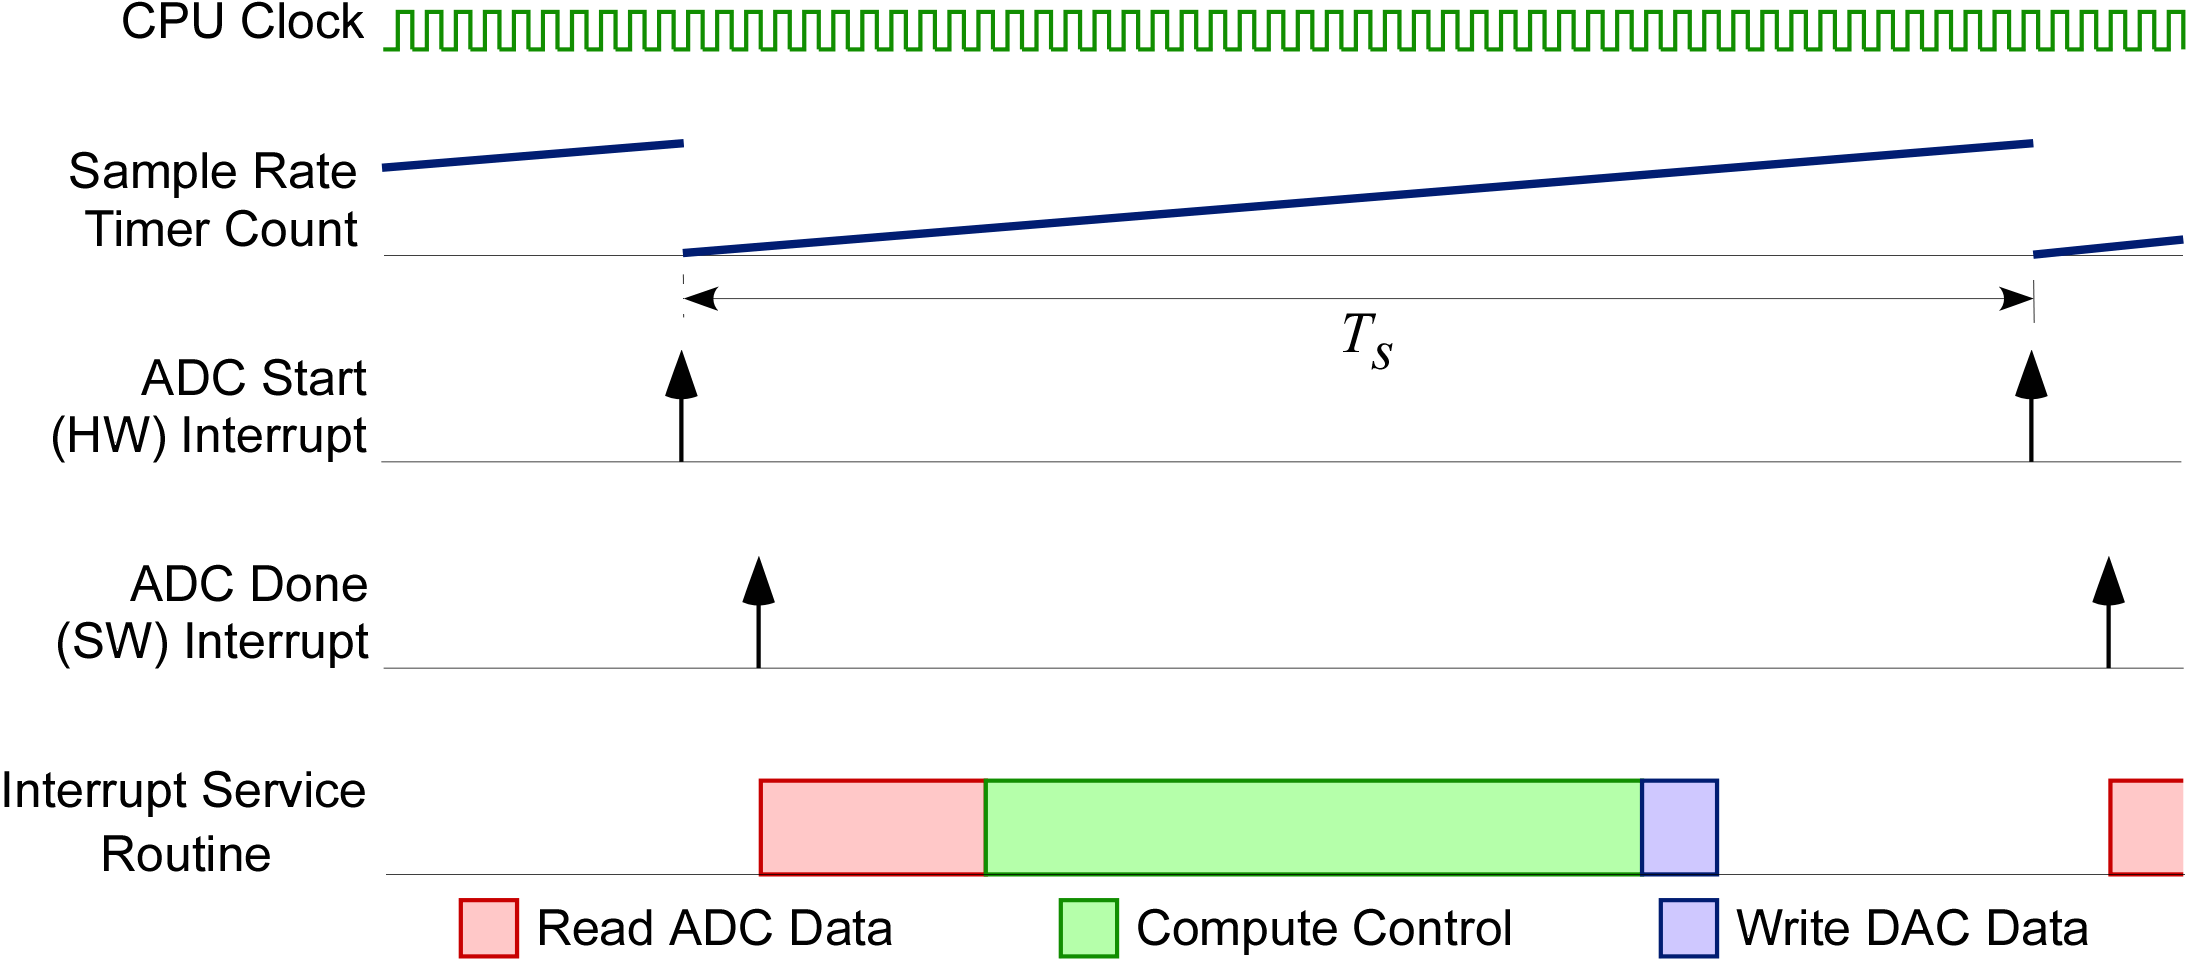
\includegraphics[width=\textwidth]{timing_diagram_large}
    \caption[Timing diagram of a real-time software loop of a \glsfmtshort{bms}]
    {Timing diagram of a real-time software loop of a \gls{bms}. The sequence of
        events within one sample period $T_s$ in relation to the base clock of
        the controller is shown. Particular emphasis is placed on depicting the
        handling of \gls{isr} requests pertinent to cell models. Other
        background tasks performed by the CPU is de-emphasised. Moreover, the
        integration of the  \gls{bms} software loop within  the larger  scope of
        a master  vehicular controller is not shown. Illustration adapted from
    Southward~\cite{Southward2011}.}
    \label{fig:timingdiagramBig}
\end{figure}

\Cref{fig:timingdiagramBig}   depicts   an   exploded   view   of   the   timing
aspects  of  the  \textsc{Interrupt  Service  Routine}  that  was  presented  in
\cref{subfig:fgRTprocess}.  Upon  the  expiry  of an  on-chip  timer  calibrated
against a  baseline precision-clock,  hardware interrupts are  raised by  one or
more \glspl{adc} associated  with voltage/current sensors mounted  on cells. The
\gls{isr}  disables  the interrupt  and  reads  the  samples  of data  from  the
\glspl{adc} into software. At the end  of this process, the \gls{isr} rearms the
interrupts  and  simultaneously sends  and  acknowledgement  to the  appropriate
sensor  which  reloads  its  timer.  The  \gls{spm}  model  equations  are  then
evaluated in software and resulting  computational variables such as voltage and
concentrations  is used  in other  activities such  as state  estimator. If  the
\gls{bms} also performs control tasks, \eg{}~regulating the coolant-flow rate or
\gls{ice} state-toggling such  as in the hysteresis control of  a series hybrid,
these control outputs are written to the relevant \glspl{dac}.


% \FloatBarrier

\subsection{Sample Delay Considerations}

\Cref{fig:timingdiagramSmall} shows a timeline view of all CPU activities across
a larger  time horizon.  The CPU's  load factor is  the ratio  of time  spent in
foreground requests to  its idling time. While a high  load factor is beneficial
in  terms of  efficient  usage  of resources,  it  adversely  affects the  power
efficiency of the chip.

\begin{figure}[!htbp]
    \centering
    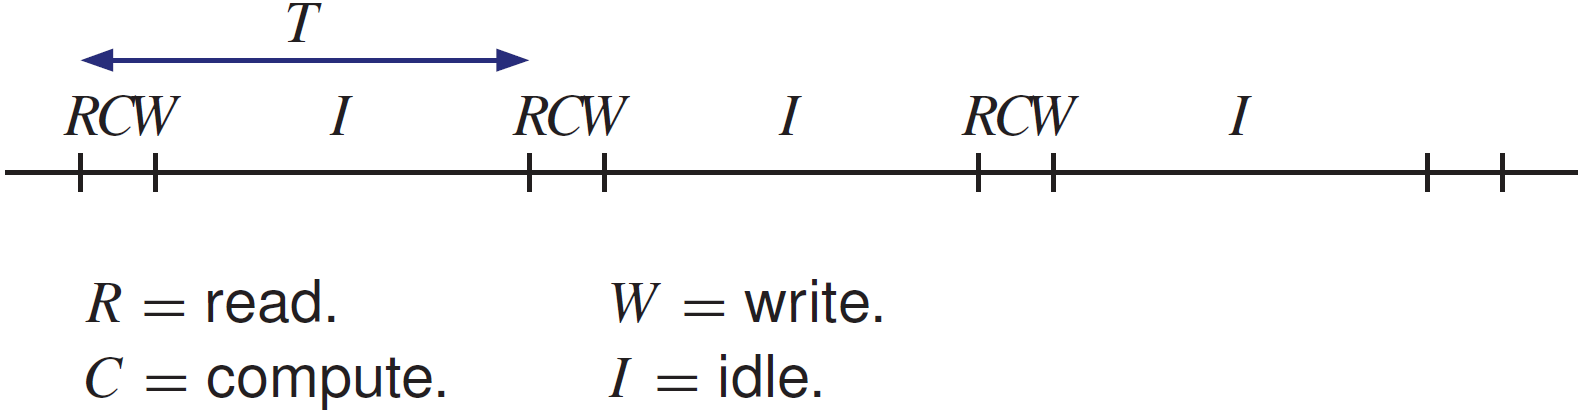
\includegraphics{timing_diagram_small}
    \caption[Timeline of \glsfmtshort{bms} activities over multiple CPU cycles of a real-time
    controller]{A compressed timeline of CPU execution cycles showing details of
        activities within each sample interval. The execution sequence is shown
        over a larger horizon so as to illustrate the proportion of `activity
        time' relative to the `idle time'. The vast majority of the CPU cycle is
        spent in idling or background tasks. The servicing of the \gls{isr}
        occupies a relatively small fraction of each CPU cycle. Diagram
    reproduced from Plett~\cite{PlettECE5540_02}.}
    \label{fig:timingdiagramSmall}
\end{figure}

For  Li-ion  cell  modelling,  a  sampling interval  of  $T_s  =  1$\si{\second}
is   commonly  used,   thus  aiming   to   capture  the   cell  dynamics   below
\SI{1}{\hertz}\footnote{In  the ideal  case, according  to the  Nyquist sampling
theorem.  In practice, the frequency  range is smaller.}. The CPUs clock is
several \si{\MHz}, a vast  majority of which is spent in  background tasks or in
sleep mode. Furthermore,  a low-latency \gls{isr} code is employed  in the tasks
of reading the  \gls{adc} value, evaluating the model equations  and writing any
control outputs to  the \gls{dac}. Using a simplified  physics-based models such
as the \gls{spm} helps in achieving a low-latency throughput for the \gls{isr}.

The overall implication of such a scheme  is that any \emph{delays} owing to the
sample and  hold process  at the model  input and outputs  can be  neglected. In
conventional sampled-data systems, control delays may be analysed by considering
a multiplicative factor of $e^{-sλ}$ in the Laplace domain transfer function of
the system.  Delay parameters of  $λ = 0.5  T_s$ or $λ  = 1 T_s$  are commonly
employed as conservative estimates. However, owing to the small CPU load factors
considered  as good  practice  in  concurrent programming,  this  delay term  is
omitted in this thesis for discrete-time formulation of the \gls{spm} model.


\subsection{Discrete-Time \glsfmtshort{spm} Formulation}

% \Cref{fig:blockdiagctsdisc} shows  a block  diagram representation of  the plant
% model its associated input and output signals.

Due  to the  sampling and  \gls{zoh} operations  at the  \gls{adc} input  to the
system,  the input  to the  \gls{spm} is  transformed from  a simple  continuous
time signal  to discrete-time  sequences \ie~\mbox{$u(t) \mapsto  u[k]$} and
\mbox{$y(t)  \mapsto  y[k]$}, where  \mbox{$k  =  0,1,\dots,∞$}~is the  sample
index  corresponding  to  the   continuous  time  instant~\mbox{$t_k  =  kT_s$}.
The  continuous  time  plant  model  represented  by  the  \gls{ode}  system  of
\cref{eq:threestatesmatrixvec} is therefore replaced  by a discrete-time process
and modelled by a \emph{difference} equation which is to be determined.

% \begin{figure}[!htbp]
%     \centering
%     % show block diagram cross-referencing equation and a question mark for the
%     % dt system
%     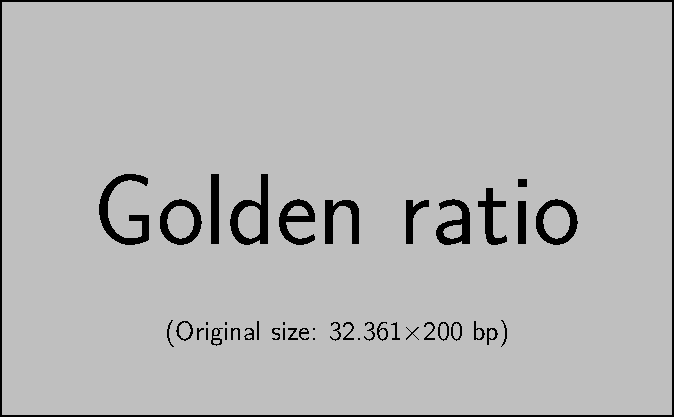
\includegraphics{placeholder_images/example-image-golden.pdf}
%     \caption[Block-diagram of continuous and discrete-time systems]{Block-diagram of the plant model and associated signals of a continuous-time system and its discrete-time counterpart}
%     \label{fig:blockdiagctsdisc}
% \end{figure}

Consider       the       general      continuous-time       solution       given
by \cref{eq:genanalyticctssoln}. Let $t_0 = k T_s$ and $t = (k+1)T_s$, where $k  =
0,1,\dots,∞$. Therefore,
\begin{alignat}{2}
    x(t_0) & = x(kT_s)     & & \equiv x[k] \\
    x(t)   & = x((k+1)T_s) & & \equiv x[k+1]
\end{alignat}
Substituting these relationships into \cref{eq:genanalyticctssoln},
\begin{equation}
    \mathbf{x}[k+1] = e^{A T_s}\mathbf{x}[k] + \int_{k T_s}^{(k+1)T_s}e^{A ((k+1)T_s-τ)}B \mathbf{u}(τ)\,dτ \label{eq:intermediatediscrete}
\end{equation}
With the  \gls{zoh} scheme  discussed here, $u(\tau)$  remains constant  from $k
T_s$ to $(k+1)T_s$,  and is equal to $u(kT_s)$ \ie~$u[k]$. Consider a change
of variable definition  for the dummy variable of integration  $\tau$ as $\eta =
(k+1)T_s -  \tau$. Thus,  $\tau = (k+1)T_s  - \eta$. Hence,  $d \tau  = -d\eta$.
Substituting these into \cref{eq:intermediatediscrete},
\begin{align}
    \mathbf{x}[k+1] &= e^{A T_s}\mathbf{x}[k] + \left[\int_{T_s}^{0}e^{A \eta }B \right] u[k]\,{-d\eta}\\
    \shortintertext{Reversing the order of integration leads to}
    \mathbf{x}[k+1] &= e^{A T_s}\mathbf{x}[k] + \left[\int_{0}^{T_s}e^{A \eta }B \,{d\eta} \right] u[k] \label{eq:disctimefulleqn}
\end{align}

\Cref{eq:disctimefulleqn} represents a discrete-time state-space representation
of the dynamics of the system whose generic representation is given by the
difference equation
\begin{equation}\label{eq:discgenericLTI}
    \mathbf{x}[k+1] = A_d x[k] + B_d u[k]
\end{equation}
where $A_d = e^{A T_s}$ and $B_d = \int_{0}^{T_s}e^{A \eta}B
\,{d\eta}$.
If the continuous-time system matrix, $A$ is invertible, a closed form
expression for $B_d$ is obtained as
\begin{align}
    B_d &= A^{-1}(A_d - I_n)B && \text{(if $A^{-1}$ exists)}
\end{align}
For the continuous time system matrix $A$ of the \gls{spm}, its determinant is
zero \ie~
\begin{equation}
\begin{vsmallmatrix}
    -30\frac{D_\spos}{R_\ppos^2} & 0                            & 0 \\
    0                            & -30\frac{D_\sneg}{R_\pneg^2} & 0 \\
    0                            & 0                            & 0
\end{vsmallmatrix} = 0
\end{equation}
and hence  is not invertible.  This necessitates  an explicit evaluation  of the
integral in \cref{eq:disctimefulleqn} for computation of the discrete-time input
matrix, $B_d$.

Since the only non-zero entries of the matrix lie along its main diagonal \ie~
its modes  are decoupled, the  matrix exponential  reduces to a  diagonal matrix
whose elements are simply the scalar exponentials of the original entries.
\begin{gather}
    A_d = e^{A T_s} = \exp\left(
        \begin{bmatrix}
            -30\frac{D_\spos}{R_\ppos^2} & 0                            & 0 \\
            0                            & -30\frac{D_\sneg}{R_\pneg^2} & 0 \\
            0                            & 0                            & 0
    \end{bmatrix} T_s \right)
    % \end{equation}
    % \begin{equation}\label{eq:A_d}
    % A_d
    =
    \begin{bmatrix}
        e^{-30\frac{D_\spos}{R_\ppos^2} T_s} & 0                                    & 0 \\
        0                                    & e^{-30\frac{D_\sneg}{R_\pneg^2} T_s} & 0 \\
        0                                    & 0                                    & 1
    \end{bmatrix} \label{eq:A_dinit} \\
    % \end{equation}
    % \begin{equation}
    B_d = \int_{0}^{T_s}e^{A \eta}B \,{d\eta}
    % \end{equation}
    % \begin{equation}\label{eq:B_dintermediate}
    % B_d
    =\bigint_{0}^{T_s} \left( \begin{bmatrix}
            e^{-30\frac{D_\spos}{R_\ppos^2} \eta} & 0                                    & 0 \\
            0                                    & e^{-30\frac{D_\sneg}{R_\pneg^2} \eta} & 0 \\
            0                                    & 0                                    & 1
        \end{bmatrix}\cdot
        \begin{bmatrix}
            \frac{45}{2} \frac{\hphantom{-}1}{R_\ppos^2 A \, l_\text{pos} a_\spos F} \\
            \frac{45}{2} \frac{-1}{R_\pneg^2 A \, l_\text{neg} a_\sneg F} \\
            \hphantom{\frac{45}{2}} \frac{-3}{R_\pneg  A \, l_\text{neg} a_\sneg F}
    \end{bmatrix} \right) \, d\eta \label{eq:B_dinit} \\
% \end{gather}
% \begin{equation}
    B_d = \begin{bmatrix}
        \hphantom{-}\frac{3}{4} \frac{1 - \exp\left(-30\frac{D_\spos}{R_\ppos^2}\right)T_s}{D_\spos A \, l_\text{pos} a_\spos F} \\[1em]
        -\frac{3}{4} \frac{1 -
        \exp\left(-30\frac{D_\sneg}{R_\pneg^2}\right)T_s}{D_\sneg A \, l_\text{neg} a_\sneg F} \\[1em]
        \hphantom{-}\hphantom{\frac{3}{4}} \frac{-3 T_s}{R_\pneg  A \, l_\text{neg} a_\sneg F}
    \end{bmatrix} \label{eq:B_d}
\end{gather}

The  discrete-time  matrix-vector  system  presented  in  \cref{eq:A_dinit}  and
\cref{eq:B_d} have  not been presented in  existing literature, but is  vital to
understanding  the  implementation  of  the \gls{spm}  in  digital  controllers.
Although, simpler  alternatives such as  Forward Euler methods are  available to
approximate the time-derivative  of the state vector, they  suffer from problems
such as increasing  rate of local truncation error  per time-step, necessitating
the use of  very high sample rates,  which increases the burden  on the embedded
controller. The matrix exponential approach is superior in terms of accuracy and
stability across a wide range of sample rates.

For a pre-determined sample-rate, the matrix exponential and hence the $A_d$ and
$B_d$  matrices  can be  computed  offline  on a  desktop  and  stored into  the
non-volatile storage  of the embedded  controller to  be loaded onto  RAM during
operation. The vectorised implementation of the state dynamics presented here is
highly  efficient  and  directly  amenable for  use  in  classical  state-vector
algorithms. For the cell's terminal voltage computation, the basic structure and
form  of the  output  equation given  by \cref{eq:spmoutputeqn} remains  intact,
except  that the  continuous time  variables $\left(\mathbf{x}(t),  u(t)\right)$
need to  be replaced  by their discrete-time  counterparts in  the corresponding
equation  set \crefrange{eq:spmbasicoutputvoltagefinal}{eq:csurfnegfromcavgneg}.
The discrete-time output  function $h_d$ is evaluated  \emph{after} updating the
state vector through \cref{eq:discgenericLTI}.
\begin{equation}\label{eq:discspmoutputeqn}
    y[k+1] = h_d(\mathbf{x}[k+1],u[k+1])
\end{equation}

The complete  sequence of steps  to implement  the discrete-time variant  of the
\gls{spm}  is given  in \cref{alg:disctimespm}. In  particular, it  can be  seen
that  the discrete-time  system  and  input matrices,  $A_d$  and  $B_d$ can  be
pre-computed  from the  parameter set  (refer to  line~\ref{algLine:computeAdBd}
in \cref{alg:disctimespm}),   using   the   matrix  exponential   approach.   In
\textsc{MATLAB}, this  can be achieved  by passing  the arguments of  the matrix
exponential to  the \verb+expm+  command. The  vectorised implementation  of the
discrete-time state equation given in line~\ref{algLine:discstateEq} is a set of
efficient linear  algebra operations consisting of  simple matrix-vector product
and vector-addition routines.

% -*- root: ../main.tex -*-
%!TEX root = ../main.tex
% this file is called up by main.tex
% content in this file will be fed into the main document
% vim:nospell

\begin{algorithm}[!htbp]
    \caption{Discrete-time \glsfmtshort{spm}}\label{alg:disctimespm}
    \addtocontents{loa}{\vskip 6pt} % https://latex.org/forum/viewtopic.php?t=6218
    \begin{algorithmic}[1]
        \Require Load profile \Comment{\eg~a \texttt{csv} file of $t$ vs.\ C-rate}
        \Require \gls{spm} parameter set  \Comment{\eg~stored in a struct \texttt{params}}
        \Userdata $z[1], t_\text{f,user}$, $t_\text{f,condition}$, cell capacity $I_\text{1C}$, sample rate $T_s$ \Comment{$t_\text{f,condition} \in  \left\{\texttt{max}, \texttt{min}\right\}$}
        \Ensure  $z[1], V_\text{cell}[1]$ within limits \Comment{index $[k=1] \wedgeq \text{time } (t=0) $}
        \Procedure{Simulate\gls{spm}}{}%{$z[1],t_\text{f,desired},T_s,I_\text{1C},\texttt{params}$}
            \State {$t_\text{f,desired} =
                \begin{cases}
                   \max(t_\text{f,user},t_\text{f,profile}),
                        &\text{%\scriptsize
                    if $t_\text{f,condition}$ == \texttt{max};}\\
                    \min(t_\text{f,user},t_\text{f,profile}),
                    &\text{%\scriptsize
                otherwise.}
                \end{cases}$} \Comment{\parbox[t]{0.25\textwidth}{may terminate early due to cut-off violations}}
                    \FullComment{\scriptsize Flexible end time. Extrapolate last C-rate from profile until $t_\text{f,desired}$ if necessary.}
            \State $N_\text{max} \gets \ceil*{\frac{t_\text{f,desired}}{Ts}} + 1$ \Comment{max iterations assuming no cut-offs}
            \State Allocate storage of size $\mathbb{R}^{N_\text{max}\times 1}$ for each simulation variable
            \State Compute $\mean{c}_\sneg$[1] as per \cref{eq:csfluxinitialcondition}
            \State $I[1] \gets I_\text{1C} \times  \text{C-rate}[1], \quad \mathbf{x}[1] \gets \vect{0,0, \mean{c}_\sneg[1]}$ \Comment{ $\text{C-rate}[1]$ from profile}
            \State \ColorLine{Compute $A_d$ and $B_d$ \Comment{as per \cref{eq:A_dinit} and \cref{eq:B_d}}}\label{algLine:computeAdBd}
            \State $V_\text{cell}[1] \gets \textsc{ComputeCellVoltage}(\textbf{x}[1],I[1],\texttt{params})$ \Comment{from direct feedthrough}
            \For{$k \gets 2 : N_\text{max}$}
                \State $I[k] \gets $ interpolate from profile using \gls{zoh}
                \State \ColorLine{$x[k] \gets A_d x[k-1] + B_d u[k-1]$ \Comment{\cref{eq:discgenericLTI}}}\label{algLine:discstateEq}
                \State Compute $z[k]$ as per \cref{eq:soccomputation}
                \State $V_\text{cell} \gets \textsc{ComputeCellVoltage}(\textbf{x}[k],I[k],\texttt{param}) $
                \If {$z[k] \text{ or } V_\text{cell}[k]$ exceeded cut-off limits}
                    \State $k \gets k - 1$ \Comment{data from last  step is invalid}
                    \State \textit{break};
                \EndIf
            \EndFor
        \EndProcedure

        \OutputEqn{\textbf{x},I,\texttt{params}} \Comment{uses discrete-time variants of eqs \ie~at index $k$}
            \State Compute $c_\snegsurf$ as per \cref{eq:csurfnegfromcavgneg}
            \Comment{consider saturating \ie~$c_\snegmin \le c_\snegsurf \le
            c_\snegmax$}
            \State Compute $\mean{c}_\spos$ as per \cref{eq:csposbulkfromcsnegbulk}
            \State Compute $c_\spossurf$ as per \cref{eq:csurfposfromcavgpos}
            \State Compute $V_\text{cell}$ as per \cref{eq:spmbasicoutputvoltagefinal}
        \EndOutputEqn%
    \end{algorithmic}
\end{algorithm}


This  thesis takes  an  inclusive view  taking into  account  that some  battery
researchers whose  focus is on fundamental  aspects of lithium ion  cells, \eg{}
those specialising in  electrochemistry, might not be familiar  with the nuances
of  the  matrix exponential  and  discrete-time  matrix computations  (refer  to
line~\ref{algLine:computeAdBd} in \cref{alg:disctimespm}).  Therefore, a snippet
of \textsc{MATLAB} code  clarifying the computation of  the discrete-time system
and input matrices, $A_d$ and  $B_d$ is given in \cref{codesnippet:computeAdBd}.
A  full code  listing of  an example  discrete-time \gls{spm}  implementation in
\textsc{MATLAB} is provided in \cref{sc:disctimespm}.

\begin{listing}[!htbp]
\begin{minted}[mathescape,autogobble,bgcolor=mintedbg,escapeinside=||,texcomments=true]{matlab}
% Returns $A_d$ and $B_d$ matrices
A_cts = [-30*Ds_pos/(R_pos^2),                    0, 0; ...
                            0, -30*Ds_neg/(R_neg^2), 0; ...
                            0,                    0, 0];
% $A_d = e^{A T_s}$ \fontfamily{libertinus}\selectfont(see \cref{eq:A_dinit})
A_disc = expm(A_cts*Ts); % $\mathtt{expm}$ command computes the matrix exponential

B_cts = [ (45/2)/(R_pos^2*a_pos*L_pos*F*A); ...
         (-45/2)/(R_neg^2*a_neg*L_neg*F*A); ...
             (-3/(R_neg*a_neg*L_neg*F*A))];

% $B_d = \int_{0}^{T_s}e^{A \eta}B \,{d\eta}$ \fontfamily{libertinus}\selectfont(see \crefrange{eq:B_dinit}{eq:B_d})
B_disc = nan(size(B_cts));
B_disc(1) = B_cts(1)*(exp(A_cts(1,1)*Ts)-1)/A_cts(1,1);
B_disc(2) = B_cts(2)*(exp(A_cts(2,2)*Ts)-1)/A_cts(2,2);
B_disc(3) = B_cts(3)*Ts;
\end{minted}
\caption{Computation of discrete-time matrices $A_d$ and $B_d$ in
\textsc{MATLAB}}
\label{codesnippet:computeAdBd}
\end{listing}

Thus,  a  discrete-time model  of  the  basic  \gls{spm}  is now  available  for
implementation  in  an embedded  \gls{bms}.  Further  analysis of  discrete-time
issues  such  as  aliasing,  quantisation  noise,  signal  pre-conditioning  and
discrete fourier analysis  lies in the specialised engineering  domain of signal
processing and falls outside  the scope of the thesis. The  results of the basic
\gls{spm} are presented next in \cref{sec:basicspmsimresults}.

% \FloatBarrier

% % https://tex.stackexchange.com/questions/113719/cleveref-fails-to-reference-algorithms

% % https://tex.stackexchange.com/questions/110412/numbering-in-algorithmicx
% % https://tex.stackexchange.com/questions/65993/algorithm-numbering

% % https://tex.stackexchange.com/questions/203713/how-can-i-typeset-function-names-as-they-appear-in-algorithmic-environments
% % https://tex.stackexchange.com/questions/100346/typesetting-listofalgorithms-like-listoffigures-and-listoftables-using-titletoc
% % https://tex.stackexchange.com/questions/30363/how-do-i-define-a-new-command-in-algorithmicx

% % https://tex.stackexchange.com/questions/67908/customizing-the-algorithmic-package-break-and-loop-labels

% % https://tex.stackexchange.com/questions/69449/avoid-putting-statements-on-the-same-line-with-algorithmicx

% % \usepackage{float}
% % \newfloat{algorithm}{t}{lop}
% % Add \floatname{algorithm}{Algorithm} to capitalise the float name


\section{Desktop Simulation}\label{sec:basicspmsimresults}
% -*- root: ../../main.tex -*-
%!TEX root = ../../main.tex
% this file is called up by main.tex
% content in this file will be fed into the main document
% vim:textwidth=80 fo=cqt

In this  section, the performance  of the  basic \gls{spm} is  discussed through
desktop  simulation and  by comparison  against a  standard \gls{dfn}  benchmark
model incorporating the full \gls{p2d} dynamics.

% \footnote{In  this   thesis,  the  terms   \gls{p2d}  and  \gls{dfn}   are  used
% synonymously.  This   is  because,   although  the  \gls{dfn}   model  equations
% are  originally  derived  and  is  applicable  in  three  dimensions,  its  most
% common  implementation  is  the  pseudo-two dimensional  case  wherein  dynamics
% of  all  variables  other  than  solid concentration  are  evaluated  along  the
% through-thickness  direction of  the  cell (direction  of  the most  significant
% charge  transport). The  solid diffusion  equation  is computed  in a  spherical
% co-ordinate system on a separate pseudo-dimension  and is coupled with the axial
% co-ordinates through the boundary flux at the surface of each particle.}

\subsection[Cell   Parametrisation]{Cell   Parametrisation\protect\footnote{Some
contents    in   this    section   overlap    with   \cref{sec:p2daugmentations}
and      represents     a      joint     effort      with     \mbox{Ian      D.\
Campbell}.}}\label{subsec:spmp2dparametrisation}

% -*- root: ../../main.tex -*-
%!TEX root = ../../main.tex
% vim:nospell

\begin{table}[!htbp]
    \small
    \caption[Simulation parameters of  an \glsfmtshort{lco} cell]{Complete set of  parameters for  isothermal simulation of the
        \gls{p2d} and  \gls{spm} implementations  of an  \gls{lco} cell  (with \ch{LiCoO_2}--\ch{LiC_6} electrode   pair
        and   \ch{LiPF_6}   electrolyte).   The  highlighted   entries represent the  parameters exclusive  to \gls{p2d}
        model.\quad  \protect{$j \in \{\text{pos},\text{sep},\text{neg}\}$}}
    \label{tbl:lcoSimParamsSPMp2d}
    \vspace{-2.6229525pt}
    \begin{threeparttable}
        \centering
        \begin{varwidth}[t]{0.48\linewidth}
            \begin{tabular*}{\textwidth}{@{} l @{\extracolsep{\fill}} r @{}}
                \multicolumn{2}{c}{\textbf{System Conditions}} \\
                \toprule
                % \multicolumn{1}{@{}l}{Parameter} \\
                % \midrule

                Lower cutoff cell voltage, $V_\text{min}$ (\si{\volt}) & \tnote{a}2.50   \\
                Upper cutoff cell voltage, $V_\text{max}$ (\si{\volt}) & \tnote{b}4.30   \\

                \bottomrule
            \end{tabular*}
        \end{varwidth}
        \hfill
        \begin{varwidth}[t]{0.48\linewidth}
            \begin{tabular*}{\textwidth}{@{} l @{\extracolsep{\fill}} r @{}}
                \multicolumn{2}{c}{\textbf{Other Constants}} \\
                \toprule
                % \multicolumn{1}{@{}l}{Parameter} \\
                % \midrule

                Faraday constant, $F$ (\si{\coulomb\per\meter})                                                        & 96487         \\
                Universal gas constant, $R$ (\si{\joule\per\mole\per\kelvin})                                          & 8.314         \\

                \bottomrule
            \end{tabular*}
        \end{varwidth}

        \smallskip
        % \vspace{-2.6229525pt}
        % \vfill
        \begin{tabular*}{\textwidth}{@{} l @{\extracolsep{\fill}} r @{}}
            \multicolumn{2}{c}{\textbf{Cell-level Parameters}} \\
            \toprule
            % \multicolumn{1}{@{}l}{Parameter} \\
            % \midrule

            Cell temperature, $T_\text{cell}$ (\si{\kelvin})                                                               & \tnote{c}298.15      \\
            \textcolor{viridistwentybluesix}{\emph{Init.}}\ electrolyte conc., $c_\text{e,0}$ (\si{\mole\per\meter\cubed}) & \tnote{c}1000        \\
            Overall active surface area, $A$ (\si{\meter\squared})                                                         & \tnote{i}\num{2.053} \\

            \bottomrule
        \end{tabular*}

        \smallskip
        \begin{tabular*}{\textwidth}{@{} =P{7.5cm} @{\extracolsep{\fill}} +l +c +r @{}}
            \multicolumn{4}{c}{\textbf{Thermodynamic, Kinetic, Geometric and Transport Parameters}} \\
            \toprule
            \multicolumn{1}{@{}l}{Parameter} & \multicolumn{1}{l}{Pos} & \multicolumn{1}{c}{Sep} & \multicolumn{1}{r@{}}{Neg}\\
            \midrule

            \rowstyle{\color{viridistwentybluesix}} Bruggeman coefficient, $\text{brugg}_j$                                                 & \tnote{c}\num{4}        & \tnote{c}\num{4}                               & \tnote{c}\num{4}        \\
            \rowstyle{\color{viridistwentybluesix}} Intrinsic electrolyte diffusivity, $D$ (\si{\meter\squared\per\second})               & \tnote{d}\num{3.22e-10} & \tnote{d}\num{3.22e-10}                        & \tnote{d}\num{3.22e-10} \\
            \rowstyle{\color{viridistwentybluesix}} Intrinsic electrolyte conductivity, $\kappa$ (\si{\siemens\per\meter})                &
            \multicolumn{3}{c}{\textcolor{viridistwentybluesix}{\Vhrulefill{} see table note \emph{e} \& \cref{subsec:basicspmsimsetup} \Vhrulefill{}}}\\
            \rowstyle{\color{viridistwentybluesix}} \ch{Li^+} transference number, $t^0_\text{+}$                                           & \tnote{c}\num{0.363}    & \tnote{c}\num{0.363}                           & \tnote{c}\num{0.363}    \\
            \rowstyle{\color{viridistwentybluesix}} Intrinsic electronic conductivity, $\sigma_j$ (\si{\siemens\per\meter})                 & \tnote{c}\num{100.00}   & ---                                            & \tnote{c}\num{100.00}   \\
            Thickness, $l_j$ (\si{\meter})                                                          & \tnote{c}\num{72e-6}    & \textcolor{viridistwentybluesix}{\tnote{c}\num{25e-6}} & \tnote{f}\num{88e-6}    \\
            Electrolyte porosity, ${\varepsilon}_j$                                                 & \tnote{c}\num{0.385}    & \tnote{c}\num{0.724}                           & \tnote{c}\num{0.485}    \\
            Filler vol.\ fraction, ${\varepsilon}_{\text{fi}_j}$                                    & \tnote{c}\num{0.025}    & ---                                            & \tnote{c}\num{0.033}    \\
            Particle radius, $R_\pj$ (\si{\meter})                                                  & \tnote{c}\num{2e-6}     & ---                                            & \tnote{c}\num{2e-6}     \\
            Specific interfacial surface area, $a_\sj$ (\si{\meter\squared\per\meter\cubed})        & \tnote{g}\num{885e3}    & ---                                            & \tnote{g}\num{723.6e3}  \\
            Electrode diffusivity, $D_{\text{s}_j}$ (\si{\meter\squared\per\second})                & \tnote{c}\num{1e-14}    & ---                                            & \tnote{c}\num{3.9e-14}  \\
            Stoichiometry, 0\% SOC, ${\theta}_{\text{min}_j}$                                       & \tnote{h}\num{0.9917}   & ---                                            & \tnote{h}\num{0.0143}   \\
            Stoichiometry, 100\% SOC, ${\theta}_{\text{max}_j}$                                     & \tnote{c}\num{0.4955}   & ---                                            & \tnote{c}\num{0.8551}   \\
            Max concentration, ${c_\text{s,max}}_j$ (\si{\mole\per\meter\cubed})                    & \tnote{c}\num{51554}    & ---                                            & \tnote{c}\num{30555}    \\
            Reaction rate coefficient, $k_\jr$ (\si{\meter\tothe{2.5}\mole\tothe{-0.5}\per\second}) & \tnote{c}\num{2.33e-11} & ---                                            & \tnote{c}\num{5.03e-11} \\
            Open circuit potential, $U_j$ (\si{\volt})                                              & \tnote{k}see table note & ---                                            & \tnote{m}see table note \\
            \bottomrule
        \end{tabular*}

        \smallskip
        % \vspace{-2.6229525pt}
        % \vfill
        %%%%%%%%%%%%%%%%%%%%%%%%%%%% SIMULATION PARAMS TABLE %%%%%%%%%%%%%%%%%%%%%%%%%%%%%
        \begin{tabular*}{\textwidth}{@{} =P{7.5cm}  +l@{\extracolsep{\fill}}+c +r @{}}
            \multicolumn{4}{c}{\textbf{Spatial Discretisation}} \\
            \toprule
            \multicolumn{1}{@{}l}{Parameter} & \multicolumn{1}{l}{Pos} & \multicolumn{1}{c}{Sep} & \multicolumn{1}{r@{}}{Neg}\\
            \midrule

            \rowstyle{\color{viridistwentybluesix}} Nodes, through-thickness (axial), $N_{\text{a}_j}$          & \num{15} & \num{15} & \num{15} \\
            \rowstyle{\color{viridistwentybluesix}} Nodes, within spherical particle (radial), $N_{\text{r}_j}$ & \num{10} & ---      & \num{10} \\

            \bottomrule
        \end{tabular*}

        % \smallskip
        % \vspace{-2.6229525pt}
        % \vfill
        \begin{tablenotes}[para,flushleft]
            \begin{scriptsize}
            \item[a] Ref.~\cite{Northrop2011}
            \item[b] Set to $\approx $\SI{100}{\milli\volt} above the cell's \gls{ocp} at \SI{100}{\percent} cell \gls{soc}
            \item[c] Ref.~\cite{Subramanian2009}
            \item[d] Computed at $T_\text{cell} = \SI{298.15}{\kelvin}$ using coefficients from table \romanletter{2} in Ref.~\cite{Valoen2005}\\%\fxnote{cross-ref to actual equation}
            \item[e] Computed at $T_\text{cell} = \SI{298.15}{\kelvin}$ using coefficients from table \romanletter{3} in Ref.~\cite{Valoen2005} at $c_\text{e,0}= \SI{1000}{\mole\per\meter\cubed}$\\
            \item[f] Set up for capacity balance of electrodes such that $l_\text{neg} = 1.22 \times l_\text{pos}$ here (see \cref{sec:electroderatio})
            \item[g] Computed as per \cref{eq:specificsurfarea}\\
            \item[h] Obtained as residual stoichiometries after a C/\num{500} simulated discharge from \SI{100}{\percent} cell \gls{soc} to \SI{2.7}{V}
            \item[i] Chosen so that current density for the electrochemical layer is \SI{29.23}{\ampere\per\meter\squared} for \SI{60}{\ampere} applied current (see \cref{sec:surfareaperlayer})
            \end{scriptsize}
            \vspace{0.5ex}
        \item[k] $ \mathcal{U(\theta_\text{pos})} = \textstyle \frac{-4.656 + 88.669\theta_\text{pos}^2 - 401.119\theta_\text{pos}^4 + 342.909\theta_\text{pos}^6 - 462.471\theta_\text{pos}^8 + 433.434\theta_\text{pos}^{10}}{-1 + 18.933\theta_\text{pos}^2 - 79.532\theta_\text{pos}^4 + 37.311\theta_\text{pos}^6 - 73.083\theta_\text{pos}^8 + 95.96\theta_\text{pos}^{10}}$ \hspace*{\fill}\refstepcounter{equation}(\theequation)\label{eq:lcoUocpPos}\\[0.25em]
            \begin{footnotesize}
            \item[m] $\mathcal{U(\theta_\text{neg})} = 0.7222 + 0.1387\theta_\text{neg} + 0.029\theta_\text{neg}^{0.5} - \frac{0.0172}{\theta_\text{neg}} + \frac{0.0019}{\theta_\text{neg}^{1.5}} + 0.2808 e^{(0.9 - 15\theta_\text{neg})} - 0.7984 e^{(0.4465\theta_\text{neg} - 0.4108)}$\hspace*{\fill}\refstepcounter{equation}(\theequation)\label{eq:lcoUocpNeg}\vfill
            \end{footnotesize}
        \end{tablenotes}
    \end{threeparttable}
\end{table}


\Cref{tbl:lcoSimParamsSPMp2d} lists  the simulation  parameters of  an \gls{lco}
cell  whose positive  and negative  electrodes are  \ch{LiCoO_2} and  \ch{LiC_6}
respectively.  The  electrolyte in  this  system  consists of  \ch{LiPF_6}~salt
in  a   solution  of   \gls{ec}/\gls{dmc}/\gls{emc}  in   a  1:1:1~ratio.  The
standard  set  of  \gls{dfn}  parameters have  been  extensively  described  and
documented  in  literature.  The   detailed  characterisation  of  the  physical
properties  of  lithium-ion  cells  falls  outside the  scope  of  this  thesis.
Here,  the vast  majority of  electrochemical parameters  \viz~the  geometric,
thermodynamic, kinetic  and transport properties  of the cell have  been sourced
from  Subramanian~\etal{}~\cite{Subramanian2009}. The  significance  of each  of
the  parameters  in  the  context  of the  modelling  assumptions  discussed  in
\cref{subsec:basicspmassumptions} is examined.

The simulation parameters that are applicable exclusively to the \gls{p2d} model
are shown as  highlighted text in \cref{tbl:lcoSimParamsSPMp2d}. It  can be seen
that only a  subset of the isothermal \gls{dfn} model's  parameters are required
for the \gls{spm}. In particular, there is no requirement to estimate any of the
electrolyte-related  parameters  in  each  electrode  region.  Furthermore,  the
properties of the separator material which  are necessary in the \gls{dfn} model
are also  not considered in the  \gls{spm} computations. A brief  enumeration of
the additional  \gls{p2d}-specific parameters in the  context of parametrisation
requirements is provided here.

\begin{enumdescriptnum}[leftmargin=!,itemsep=1ex,labelwidth=\widthof{$\symbf{\text{brugg}_j}\ \scriptstyle (\times 3)$abc}
    ,partopsep=0pt
    ,topsep=0pt
    ]

    \customenum{\text{brugg}_j}{3}  The  empirical Bruggeman  coefficient  helps
    to   define   the  effective   values   of   conductivity  and   diffusivity
    of   the  electrolyte.   Although  an   identical  value~(4)   is  used   in
    \cref{tbl:lcoSimParamsSPMp2d},  in  principle  all three  regions  can  have
    different values of brugg and need to be parametrised separately.

    \customenum{D}{1}  The  intrinsic  electrolyte   diffusivity  of  a  typical
    electrolyte  consisting  of  \ch{LiPF_6}~salt in  an  organic  solvent  was
    experimentally  characterised   and  provided  as  a   table  of  polynomial
    coefficients  by  Valøen  and  Reimers~\cite{Valoen2005}.  Evaluating  this
    polynomial  at a  cell  temperature of  \SI{298.15}{\kelvin}  results in  an
    intrinsic  diffusivity  of~\SI{3.22e-10}{\meter\squared\per\second}.  Since
    this is  a material property independent  of the region within  the cell, it
    needs to be parametrised only once.

    \customenum{\scalebox{1.35}{$\kappa$}}{1}   Like    the   diffusivity,   the
    intrinsic electrolyte conductivity is also a material property and its value
    is independent  of the region within  the cell. Unlike the  diffusivity, the
    electrolyte conductivity  is a strong  function of its  ionic concentration.
    Thus, the polynomial proposed by Valøen and Reimers~\cite{Valoen2005} needs
    to  be evaluated  at~$T_\text{cell}= \SI{298.15}{\kelvin}$  and  has to  be
    updated during the  simulation as salt concentration  within the electrolyte
    changes over time. A discussion on the choice of initial concentration is
    provided in \cref{subsec:basicspmsimsetup}.

    \customenum{\scalebox{1.25}{$t$}_+^0}{1}  The  cationic transference  number
    measures the relative  mobility of the \ch{Li^+}~ion in  the organic solvent
    and is  independent of  the region  within the  cell. Hence,  this intrinsic
    property is to be parametrised only once (per solvent).

    \customenum{\scalebox{1.25}{$\sigma$}_j}{2}  The  intrinsic conductivity  of
    the  solid phase  depends on  the material  used in  the porous  electrodes.
    Although a simplified  assumption of equal conductivity is used  for the two
    electrodes, in practice, this property needs to be characterised for each of
    the two electrodes.

\end{enumdescriptnum}

\sisetup{detect-weight=true}  Neglecting  Arrhenius-type temperature  dependence
of  physical  properties  and   their  corresponding  activation  energies,  the
basic  \gls{spm}  facilitates  the  ability to  afford  physics-based  modelling
capabilities with  \emph{eight} fewer parameters than  the equivalent isothermal
\gls{p2d} model. With  the naive assumption of equal  parametrisation effort per
physical property, this  implies a \textbf{\SI{20}{\textbf{\percent}}} reduction
in  parametrisation  requirements  for  the basic  \gls{spm}  when  compared  to
its  \gls{dfn} counterpart.  However,  considering the  fact that  parametrising
the  electrolyte's transport  properties requires  apparatus and  infrastructure
typically  available only  in specialised  chemical/materials~science labs,  the
reduction in parametrisation overhead  for system-level engineering stakeholders
is more pronounced.

Prima~facie, it may seem that electrolyte porosities and filler volume fractions
do  not  influence the  \gls{spm}  model.  However,  they  do have  an  indirect
bearing  on  arriving  at  a  critical parameter  \viz~the  solid  phase  volume
fraction~$\varepsilon_\sj$. This  parameter is required to  compute the specific
interfacial surface  area of the electrodes~$a_\sj$  \ie~the effective electrode
area  exposed to  reaction and  is an  important entity  in the  \gls{spm} model
equations  presented  in  \cref{subsec:basicspmgoverningeqns}. The  solid  phase
volume fractions  are also required in  simulating the \gls{p2d} model  owing to
the need for computing the effective electronic conductivities of the electrodes
(see \cref{eq:solidchargeconserve}). They are calculated as
\begin{equation}\label{eq:volumefraccalc}
    \varepsilon_\sj = 1 - \varepsilon_j - \varepsilon_{\text{fi}_j}
\end{equation}
where~$\varepsilon_j$  and~$\varepsilon_{\text{fi}_j}$  are the  electrolyte and
filler  volume-fraction  within  the  respective electrode  regions.  Using  the
values from \cref{tbl:lcoSimParamsSPMp2d} results in~${\varepsilon_\spos =
0.590}$
and  ${\varepsilon_\sneg  =  0.482}$~for the  positive  and  negative  electrodes
respectively. The specific interfacial surface areas are then calculated as
\begin{equation}\label{eq:specificsurfarea}
    a_\sj = \varepsilon_\sj \frac{4 \pi R_\pj^2}{\frac{4}{3} \pi R_\pj^3} = \frac{3\varepsilon_\sj}{R_\pj}
\end{equation}

As   discussed  in   the   assumptions  made   during   model  derivation   (see
\cref{subsec:basicspmassumptions})  and   consistent  with  the   assumed  model
geometry,  the  parameters  not  covered  by  the  \gls{spm}  pertain  to  those
describing electrolyte dynamics and distribution  of electronic charge along the
axial  thickness  direction  of  the  cell. Properties  such  as  the  intrinsic
diffusivities and conductivities of the  electrolyte as well as the transference
number of  \ch{Li^+} in the  organic solvent  are thus completely  redundant for
\gls{spm}  simulation.  The  assumption  of uniform  charge  density  along  the
through-thickness length of each electrode implies that the intrinsic electronic
conductivities of the two electrodes do not play any role in the model dynamics.
The porosities and Bruggeman coefficients in \cref{tbl:lcoSimParamsSPMp2d} serve
as  modifying factors  of the  intrinsic conductivities  and diffusivities  (see
\cref{tbl:dfneqns})  leading to  an effective  value within  each region  of the
electrochemical  layer. Thus,  their relevance  is  also rendered  void for  the
basic  \gls{spm}  simulation.  The  thickness of  the  separator  material  only
plays  a role  in  electrolyte behaviour.  By the  model  geometry presented  in
\cref{subsec:basicspmgeometry}, this  parameter also falls outside  the scope of
the basic \gls{spm}.

The  thicknesses  of the  electrodes  are  optimised  for equal  loading  \ie~to
achieve   a  balance   in   their  individual   capacities   to  store   \ch{Li}~atoms.  The  thickness  of  the  positive  electrode  is  chosen  as  the  value
from~Subramanian~\etal{}~\cite{Subramanian2009}. The  thickness of  the negative
electrode region  is then  computed with  the goal of  equalising the  volume of
active material  in each electrode  for every  electrochemical layer in  a pouch
cell.
\begin{equation}\label{eq:basiccapacitybalance}
    A_{\text{elec}_\text{pos}}\varepsilon_\spos l_\text{pos} = A_{\text{elec}_\text{neg}}\varepsilon_\sneg l_\text{neg}
\end{equation}

In a  lithium-ion pouch cell, the  electrodes are designed such  that the layers
can be  overlaid on  top of  one another  and finally  encapsulated in  a pouch.
Geometrical considerations  then imply  that the  cross-sectional area  (or face
area) of the two electrodes must be  the same. However, due to the consideration
of  avoiding  plating  at  the  edges  due  to  microscopic  malformations,  the
design  is done  such as  to have  a small  overhang of  the negative  electrode
layer~${(<  \SI{2}{\milli\meter})}$  with  respect  to  the  positive  electrode
layer~\cite{Bond2017} (see \cref{fig:anodeoverhangpouchcell}). Nevertheless, the
active surface area is just the  common overlap area between the two electrodes,
and hence $A_\text{elec}$~is  equal to the cross-sectional area  of the positive
electrode.

Thus, \cref{eq:basiccapacitybalance} reduces to~${\frac{l_\text{neg}}{l_\text{pos}} =
\frac{\varepsilon_\text{pos}}{\varepsilon_\text{neg}} = 1.22}$,~yielding~${l_\text{neg} = \SI{72}{\micro\meter}}$.

At  first,  it may  be  surprising  to note  that  the  values of  the  particle
radius~$R_\pj$  used  in both  the  \gls{p2d}  and \gls{spm}  remain  identical.
However, it is  important to note that the \gls{p2d}  equations of the \gls{dfn}
model  are cast  in a  normalised form  \ie~already set  up to  account for  the
overall capacity of  the cell under consideration implicitly through  usage of a
current density (per  unit area) for its simulation.  Furthermore, this explains
why increasing the number of discretisation nodes does not increase the modelled
capacity, but instead merely serves to improve the simulation accuracy owing to
the enhanced spatial resolution.

The  overall  active  surface  area~${A  = n  A_\text{elec}}$  is  the  combined
cross-sectional area of  all layers ($n$~is the number  of electrochemical (pos,
sep,  neg)  triplets)  stacked  into  the pouch  cell.  In  both  the  \gls{p2d}
and  \gls{spm}  models,  this  parameter  serves  to  scale  the  external  load
current  down  to  the  current  density  experienced  by  each  electrochemical
layer.  A   value  of  \approx\SI{30}{\ampere\per\meter\squared}   was  reported
in  the  results  section  of  Subramanian~\etal{}~\cite{Subramanian2009}.  When
considering a  \SI{60}{\amphour} pouch cell with  \SI{10}{\milli\meter} exterior
thickness   and  using   the   parameters  reported   in~\cite{Subramanian2009},
this  results  in  a  cross-sectional area  of  \SI{2.053}{\meter\squared}  (see
\cref{sec:p2daugmentations}). Considering the  equalisation of capacity loading,
with the  newly chosen thickness  value of  the negative electrode,  the 1C-rate
capacity of the cell has been revised to~\SI{29.23}{\ampere\per\meter\squared}.

On  simulating  the \gls{p2d}  model  with  a  trickle bleeding  type  discharge
corresponding   to   a  current   of   C/500   and   logging  the   data   every
\SI{1}{\milli\second}, after reaching \SI{2.7}{\volt}\footnote{From manufacturer
datasheets  for \protect{\gls{lco}}  chemistries,  this value  is considered  to
correspond to~\SI{0}{\percent} \protect{\gls{soc}}.}, the remnant concentrations
in  the two  electrodes  were noted.  The  corresponding residual  stoichiometry
values are reported in \cref{tbl:lcoSimParamsSPMp2d}.

% and is  consistent with  typical values reported  in literature  for \gls{lco}
% chemistries.\fxnote{citation needed here.} This validation is important, since
% below certain  stoichiometry thresholds,  the spinel/olivine structure  of the
% electrodes can become unstable and collapse\fxnote{citation needed?}.

Since      only      isothermal      cell     behaviour      is      considered,
\cref{tbl:lcoSimParamsSPMp2d}    omits     the    activation     energies    for
the    various   diffusivities    and   conductivities    of   materials    (see
\cref{subsec:basicspmsimsetup}  for further  thermal  considerations). For  this
reason, \cref{tbl:lcoSimParamsSPMp2d} does not include other material properties
such as specific heats, and thermal conductivities. No properties of the current
collectors appear in  the isothermal model equations for both  the \gls{p2d} and
\gls{spm} models  and hence are  omitted. All other  electrochemical properties,
\viz~stoichiometries  at \SI{100}{\percent}  \gls{soc}, maximum  concentrations,
diffusivities, reaction  rate coefficients and  \gls{ocp} of the  two electrodes
remain invariant between the \gls{p2d} and \gls{spm} models.

\subsection{Simulation Setup}\label{subsec:basicspmsimsetup}

For  reproducibility of  results, it  is important  to discuss  the system-level
parameters influencing simulation setup.

The lower  cut-off voltage  of the  cell is chosen  to be~\SI{2.5}{\volt}. This
is  deliberately  kept  lower  than  the voltage  corresponding  to  the  cell's
\SI{0}{\percent}~\ie~\SI{2.7}{\volt}.  If set  above  \SI{2.7}{\volt}  even
at  infinitesimally small  discharge  currents, the  cell  would cut-off  before
achieving complete discharge. Choosing a value lower than \SI{2.7}{V} means that
the cell gets a chance to recover its terminal voltage, despite spikes in highly
dynamic  load  currents  that  might  bring the  voltage  below  this  threshold
momentarily. If a low-enough value is  not chosen, a system-level shutdown shall
be  initiated  despite possessing  the  ability  to  continue to  operate  after
recovery  of terminal  voltage.  In this  case, choosing  a  cut-off voltage  of
\SI{2.5}{\volt} does  not damage the cell  since checks are in  place to monitor
the  \gls{soc}  and trigger  cut-off  in  the  event  of charge  depletion  (see
\cref{alg:ctstimespm,alg:disctimespm}).  Northrop~\etal~\cite{Northrop2011}  use
this value, although no specific explanation is given for this choice.

The  upper   cut-off  voltage   of  the  cell   is  chosen   at  \SI{4.3}{\volt}
\ie~\approx\SI{100}{\milli\volt} higher  than  the  equilibrium \gls{ocp}  at~\SI{100}{\percent} \gls{soc}. There are several  reasons for this smaller margin
at the upper end of the voltage spectrum.
\begin{description}[leftmargin=!,labelwidth=\widthof{\bfseries low
    probabilities},itemsep=1ex]

\item[safety] li-ion  cells are less  tolerant to overcharging and  can pose
    fire hazards.

\item[degradation]  overcharging  li-ion  cells  can  lead  to  plating  and
    accelerate other degradation mechanisms.

\item[low  C-rates]  charging C-rates  are  typically  lower than  discharge
    C-rates.

\item[CCCV charging]  For on-board  chargers, taper charging  (such as  in a
    \gls{cccv} profile) is activated, which  ensures that charging current drops
    off  rapidly, leading  to a  lower overvoltage  towards the  upper \gls{soc}
    range.

\item[low probabilities] The only charging event when an electrified vehicle
    is in motion is during regenerative braking. The vehicular \gls{bms} manages
    the operating window such that the starting \gls{soc} is much lower than the
    overvoltage  that  could  be  caused due  to  braking.  Furthermore,  during
    operation, net discharge events  occur more frequently than regenerative
    braking events.

\end{description}

For  both the  \gls{p2d} model  and the  \gls{spm} model,  the cell  temperature
is   kept   constant   at   its   initial   value   of   \SI{25}{\degreeCelsius}
(\SI{298.15}{\kelvin}). This might imply to the reader that the operation of the
lithium ion cell is assumed to be isothermal. While this is not true in general,
for  the C-rates  considered  here  (<5C), typical  in  a \gls{bev}  application
particularly for the  short-duration transient loads studied, it  is certainly a
valid  zeroth  order  coarse  approximation of  the  cell's  thermal  condition.
Detailed modelling of  thermal dynamics is not within the  scope of this thesis,
as  the primary  goal is  to  obtain a  \gls{pbm} incorporating  electrochemical
principles amenable for  embedded application. Hence, the  thermal dependence of
parameters through an Arrhenius-type relationship is also not considered. Future
work could  include performing  thermally coupled  simulations \ie~incorporating
thermally dependent parameters and  simplified heat generation expressions \eg~a
lumped thermal model could be employed  for both the \gls{spm} and \gls{p2d} and
their performances may be compared.

To  understand  the parametrisation  of  initial  concentration, the  expression
for   electrolyte  conductivity   needs  to   be  examined.   As  discussed   in
\cref{subsec:spmp2dparametrisation},  the intrinsic  conductivity of  a specific
type  of  electrolyte  is  a  material   property  that  depends  on  the  local
concentration of \ch{Li^+}~ions and temperature.  In the characterisation of the
electrolyte by  Valøen and  Reimers~\cite{Valoen2005}, the best  fit expression
for electrolyte conductivity was obtained as
\begin{multline}\label{eq:kappavsCeandT}
    \kappa_j(c_\text{e},T)(x,t) =  10^{-4} c_\text{e}(x,t) \bigl(-10.5 + \num{0.668e-3} c_\text{e}(x,t) + \num{0.494e-6}  c_\text{e}{(x,t)}^2\\
    + (0.074 - \num{1.78e-5}) c_\text{e}(x,t) - \num{8.86e-10} c_\text{e}{(x,t)}^2 \bigr)T(t)\\
	+ \left(\num{-6.96e-5} + \num{2.8e-8} c_\text{e}{(x,t)})T(t)^2\right)^2
\end{multline}

\begin{figure}[!htbp]
    \centering
    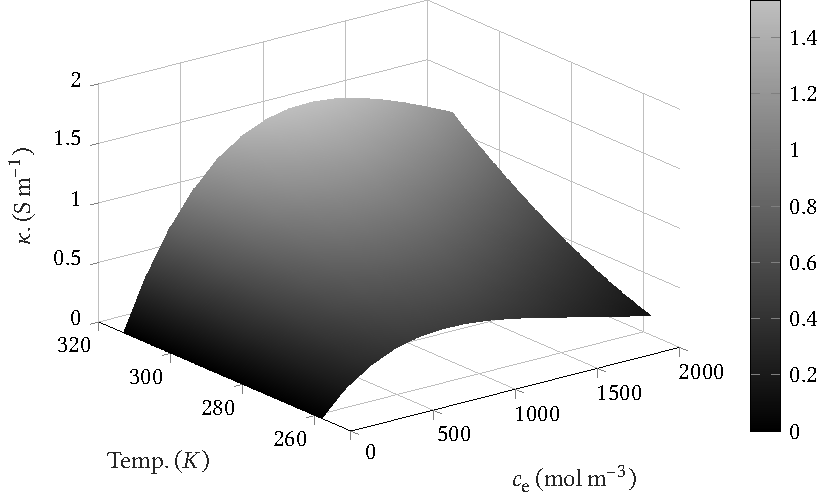
\includegraphics{m2t_kappa_ce_T.pdf}
    \caption[Surface plot of electrolyte conductivity]
    {Electrolyte conductivity as a function of cell temperature and initial concentration.
        % The variation of conductivity versus these factors is a smooth function.
    }%
    \label{fig:kappavsCeandT}
\end{figure}

\Cref{fig:kappavsCeandT}   shows    a   surface   plot   of    the   electrolyte
conductivity  as a  function  of initial  concentration~$c_\text{e,0}$ and  cell
temperature~$T_\text{cell}$. For the modelling task at hand, relevant aspects of
this  material property  can be  better understood  through the  simplifications
afforded by  the simulation conditions  applicable here. At  equilibrium initial
condition,  $c_\text{e}$~is uniform  over  the axial  space~$x$. Secondly,  only
isothermal  cell   behaviour  is   considered  \ie~${T(t)   =  T_\text{cell}(0)=
T_\text{cell}}$. Hence, \cref{eq:kappavsCeandT} reduces to
\begin{multline}\label{eq:kappavsCeinitandTcell}
    \kappa_j =  10^{-4} c_\text{e,0} \bigl(-10.5 + \num{0.668e-3} c_\text{e,0} + \num{0.494e-6}  c_\text{e,0}^2\\
        + (0.074 - \num{1.78e-5}) c_\text{e,0} - \num{8.86e-10}
    c_\text{e,0}^2 \bigr)T_\text{cell}\\
	+ \left(\num{-6.96e-5} + \num{2.8e-8} c_\text{e,0})T_\text{cell}^2\right)^2
\end{multline}

As inferred from \cref{fig:kappavsCeandT}, the electrolyte conductivity~$\kappa$
is    a    smooth    function    of~$c_\text{e}$    and~$T_\text{cell}$.    Thus
\cref{eq:kappavsCeinitandTcell}   can  be   effectively  visualised   through  a
parametric  plot of  $\kappa$ versus  $c_\text{e}$ with  $T_\text{cell}$ as  the
variable parameter  as seen in \cref{fig:kappavsce}.  From \cref{fig:kappavsce},
it  is  evident   that  at~${T_\text{cell}=\SI{298.15}{\kelvin}}$,  the  maximum
value   of    electrolyte   conductivity    is   attained    at~${c_\text{e}   =
\SI{1000}{\mole\per\meter\cubed}}$.  It  is  advantageous to  operate  the  cell
around  this   salt  concentration  so   as  to  minimise  the   cell's  overall
resistance.  Hence, the  initial  concentration~$c_\text{e,0}$ is  chosen to  be~\SI{1000}{\mole\per\meter\cubed}. It should be  noted that while the electrolyte
concentration  in  the  \gls{p2d}  model  exhibits  both  spatial  and  temporal
variations during  the simulation, in  the \gls{spm} model, it  remains constant
throughout.

\begin{figure}[!htbp]
    \centering
    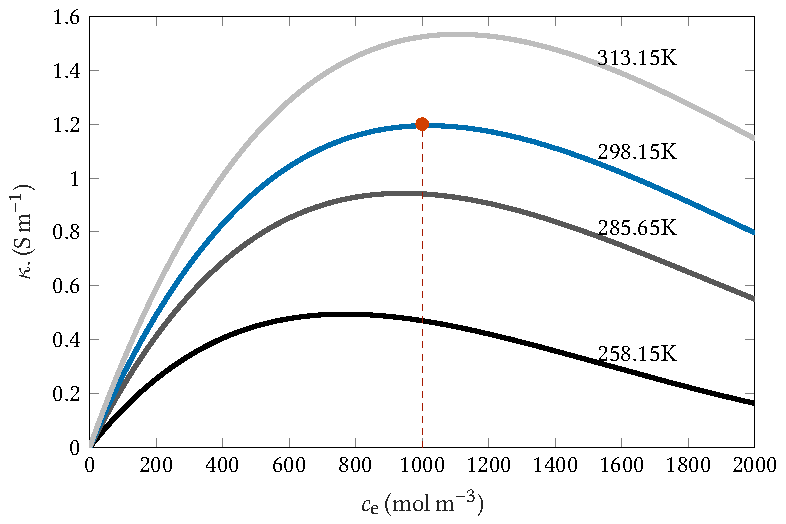
\includegraphics{m2t_kappa_ce_parametric_T.pdf}
    \caption[Electrolyte conductivity versus concentration at various cell
    temperatures]{Electrolyte conductivity versus equilibrium concentration at
        various cell temperatures. At~${T_\text{cell} = \SI{298.15}{\kelvin}}$,
        the maximum value of electrolyte conductivity corresponds to a salt
    concentration of~\SI{1000}{\mol\per\meter\cubed}.}
    \label{fig:kappavsce}
\end{figure}

The     reduction    in     parametrisation     requirements    discussed     in
\cref{subsec:spmp2dparametrisation}    is    only    one    of    the    factors
contributing  to  the  simplicity  and  ease  of  simulation.  As  discussed  in
\cref{subsec:basicspmgeometry}, an  important computational requirement  that is
present in the \gls{p2d} model, but  completely eliminated from the \gls{spm} is
the requirement of discretisation. As reported in \cref{tbl:lcoSimParamsSPMp2d},
with  15~nodes per  region  along the  axial direction  and  with 10~shells  per
electrode in the radial direction, the \gls{p2d} model under simulation achieves
mesh  independence  to  a  tolerance of~\approx\SI{2}{\percent}  for  the  range
of  C-rates  considered.  For  higher  C-rates,  coupling  a  thermal  model  is
of  higher  importance  than  incorporating  further  meshing  refinements.  The
discretisation-related parameters  are specific to  the \gls{p2d} model  and are
highlighted accordingly in \cref{tbl:lcoSimParamsSPMp2d}.

\subsubsection*{Capacity Characterisation}\label{subsubsec:capcharspmp2d}

First, it  must be  established that incorporating  the parameters  presented in
\cref{tbl:lcoSimParamsSPMp2d} into  the \gls{spm}  model equations results  in a
cell with  \emph{identical} capacity as the  \gls{dfn} model. This is  to ensure
the  validity  of  comparisons  in  further simulations.  Using  the  values  of
per-layer C-rate  as discussed  in \cref{subsec:spmp2dparametrisation},  and the
overall active  surface area from \cref{tbl:lcoSimParamsSPMp2d},  the cell under
simulation has a capacity of~\SI{60}{\amphour}.

Present literature  in battery modelling, both  for the \gls{dfn} model  and for
the  \gls{spm}, do  not  discuss  any aspect  of  capacity characterisation.  In
particular,  parameters  such  as  the  geometric  surface  area  of  cells  and
even  their 1C-rate  are often  not listed  in publications.  This practice  can
be  attributed  to  the  fact  that  all  one-dimensional  and  \glsfmtlong{p2d}
models operate  on a per-layer  basis, using an applied  current \emph{density}.
Many  a  time,  researchers assume  a  unit  surface  area  for the  cell.  This
implicit  normalisation  is amenable  to  those  studies  which strive  to  make
numerical comparisons  between models through  simulation. However, it  leads to
a  lack  of  clarity  on  the  actual capacity  of  the  cells  being  modelled.
Furthermore, when comparing with experimental data  from a real cell, such works
resort to  \mbox{ad hoc} techniques such  as empirical curve-fitting for  obtaining the
surface  area. Often  the  source of  such parametrisation  is  not made  clear.
\Cref{sec:p2daugmentations}  documents  the  details of  obtaining  the  overall
surface area  of cells  and arriving  at the  C-rate per  layer of  the specific
cell  under  consideration.  Since  the  \gls{dfn}  model  does  not  explicitly
model  the cell  capacity,  a brief  explanation  is provided  on  how a  simple
\emph{numerical}  characterisation can  be  used for  determining cell  capacity
given a \emph{complete} parameter list.

%\fxnote{citations needed for each accusation.}

For experimental capacity characterisation of cells, the standard practice is to
apply a very small discharge  current beginning at \SI{100}{\percent} \gls{soc},
logging the charge passed using a  high-precision coulomb counter until the cell
hits the voltage corresponding to \SI{0}{\percent} \gls{soc} as specified in the
manufacturer's datasheet. In order to decouple the effect of the cell's dynamics
from its  capacity, it is  required to  apply an infinitesimal  bleeding current
(tending towards, but not reaching \SI{0}{\ampere}).

Current sensors in battery cycler equipment use high-precision (typically 15--18
bit) \glspl{adc}  and are  able to  offer high  \glspl{snr} except  at ultra-low
currents. The main difficulty with using very low C-rates is that it drastically
slows down  the characterisation procedure.  Using a discharge  current of~C/100
\ie~\SI{0.6}{\ampere}  in  this case,  results  in  a characterisation  time  of
\SI{100}{\hour} or \mbox{\approx 4$\sfrac{1}{4}$}~days (excluding soak-times and
other set-up related activities).  Furthermore, for accurate coulomb-counting, a
high data logging  rate is needed, producing large file  sizes and corresponding
difficulties in post-processing them.  Considering moderate buffer-sizes used in
data logging modules of typical  cell-cycler software (shared between channels),
and  to  avoid  excessively  large wait-times  for  characterisation,  discharge
currents of C/20--C/25 are usually deemed sufficient.

In    order   to    validate    that   the    choice    of   model    parameters
result   in   an   intended   capacity  of   \SI{60}{\amphour},   an   analogous
procedure   is    carried   out   by    means   of   computer    simulation.   A
characterisation  simulation  beginning  at  \SI{100}{\percent}  \gls{soc}  with
a   discharge   current    of   \SI{0.6}{\ampere}   was   performed\footnote{All
computations  were  performed  on   a  64-bit  Hewlett-Packard~Z840  workstation
with   a   \mbox{16-core}   \mbox{\text{Intel}\textsuperscript{\textregistered}}
\mbox{Xeon\textsuperscript{\textregistered}}     \mbox{E5-2640~v3}     (Haswell)
processor clocked  at \SI{2.60}{\giga\hertz} with  \SI{128}{\giga\byte} DDR4~RAM
at 1866~MT/sec.}.  If the assumed  cell capacity  is indeed consistent  with the
model parameters,  then this corresponds to  a C-rate of~1/100.  Therefore, both
the \gls{p2d} and \gls{spm} should run  for exactly 100~hours before cut-off due
to charge depletion.


Capacity validation through computer simulation  is not bound by the limitations
of the experimental approach discussed earlier. Using 64-bit IEEE floating point
arithmetic,  quantities  as  low  as  ${\mathcal{O}(10^{-16})}$  can  be  safely
computed, nullifying  any \gls{snr} issues.  \Cref{tbl:charSimspmp2d} summarises
the key data  from this simulation run. For accurate  coulomb counting, the data
logging  interval is  set to~\SI{50}{\milli\second}.  Both models  ran close  to
100~hours.  The small  deviations from  this  expected termination  time can  be
attributed  to the  fact that  the  current is  not arbitrarily  small with  the
pragmatic goal of obtaining results in a reasonable time.

% -*- root: ../main.tex -*-
%!TEX root = ../main.tex
% this file is called up by main.tex
% content in this file will be fed into the main document
% vim:nospell

\begin{table}[!htbp]
    \centering
    \caption[Simulation data for capacity characterisation of \glsfmtshort{p2d} and \glsfmtshort{spm} models]{Simulation data for capacity characterisation of \glsfmtshort{p2d} and \glsfmtshort{spm} models. The \glsfmtshort{p2d} model is considered as the reference benchmark. The modelling error is defined as \protect{$\varepsilon_v = V_{\text{cell}_\text{p2d}} - V_{\text{cell}_\text{spm}}$}}
    \label{tbl:charSimspmp2d}
    \begin{tabular}{@{} l r r @{}}
        \toprule
        Parameter                                                               & Value  & Units              \\
        \midrule
        Data-logging interval                                                   & 50.00  & \si{\milli\second} \\
        Combined CPU time with warm cache                                       & 12.22  & \si{\minute}       \\
        Total RAM used                                                          & 603.90 & \si{\mega\byte}    \\
        \glsfmtshort{p2d} run-time                                              & 99.94  & \si{\hour}         \\
        \glsfmtshort{spm} run-time                                              & 99.90  & \si{\hour}         \\
        \glsfmtshort{p2d} discharge capacity                                    & 59.96  & \si{\amphour}      \\
        \glsfmtshort{spm} discharge capacity                                    & 59.94  & \si{\amphour}      \\
        Worst case error, $\varepsilon_{v_{\text{max}}}$                        & -94.30 & \si{\milli\volt}   \\
        Mean error, $\mu_{\varepsilon_v}$                                       & -3.00  & \si{\milli\volt}   \\
        \glsfmtshort{rms} error, $\varepsilon_{v_{\,\text{\glsfmtshort{rms}}}}$ & 8.20   & \si{\milli\volt}   \\
        \glsfmtshort{mae} error, $\varepsilon_{v_{\,\text{\glsfmtshort{mae}}}}$ & 3.20   & \si{\milli\volt}   \\
        Standard deviation of error, $\sigma_{\varepsilon_v}$                   & 7.60   & \si{\milli\volt}   \\
        \bottomrule
    \end{tabular}
\end{table}


As seen in \cref{tbl:charSimspmp2d}, even  the \emph{combined} \gls{cpu} time to
simulate both  the \gls{p2d}  and \gls{spm}  models is  two orders  of magnitude
lower than  real-time. The only  issue that remains to  be addressed is  that of
considerable memory and  storage requirements due to  high-rate data-logging for
accurate coulomb counting. For a standard computer workstation, this places only
a minor demand on its \gls{cpu}. For comparable volume of data to be logged, the
reliability  and ruggedness  of  a  dedicated workstation  far  exceeds that  of
real-time cell cyclers, thereby establishing numerical simulation as an amenable
method for characterisation of cell capacity. A major disadvantage of simulation
based capacity validation  is its extreme sensitivity to parameters  such as the
maximum concentration  of the  electrodes and  their stoichiometries,  which are
generally difficult to characterise. In this context, the experimental procedure
of  high-precision  coulomb counting  assumes  a  practical significance  as  it
requires no  knowledge of  the cell's parameters  other than  the manufacturer's
datasheet.


\Cref{fig:capcharspmp2d}  shows  the  voltage  response  of  the  \gls{spm}  and
\gls{p2d}  models,  which   overlap almost entirely.  It  is  clear  that   both  the  \gls{p2d}
and  \gls{spm}  models   achieve  a  run-time  of   100~hours.  This  represents
the   first  visualisation   of  results   produced  by   the  \gls{spm}   model
equations  discussed  in \cref{subsec:basicspmgoverningeqns} and  its  numerical
implementation  from \cref{sec:numericalimplementation}.

\begin{figure}[!htbp]
    \centering
    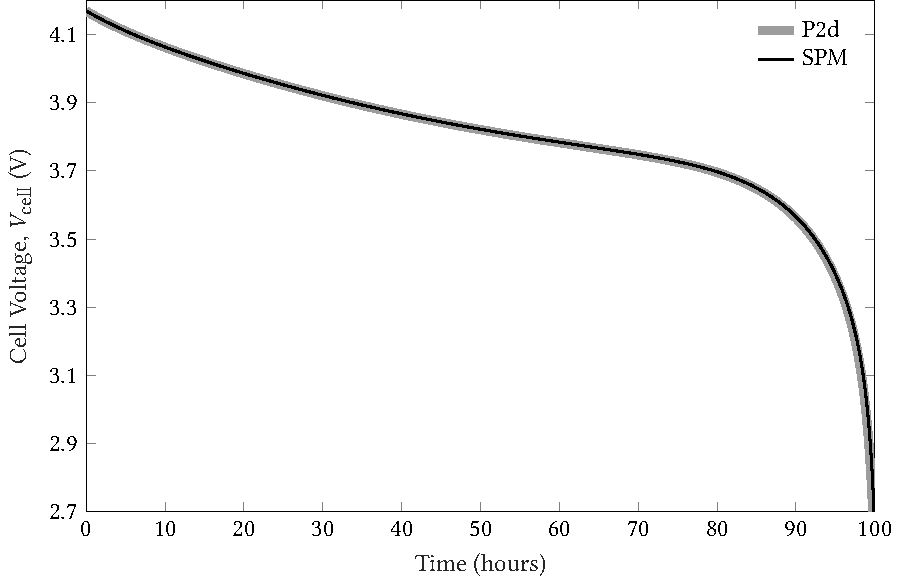
\includegraphics{capacity_match_spm_p2d.pdf}
    \caption[Voltage response of \glsfmtshort{spm} and \glsfmtshort{p2d} models
    for capacity validation]{Voltage response of \gls{p2d} and \gls{spm} models
        to a discharge current input of~\SI{0.6}{A}. Both models achieve their
        charge depletion point after \approx\SI{100}{\hour} confirming that
        their modelled capacities match. Key simulation data for this
    characterisation run is shown in \cref{tbl:charSimspmp2d}.}
    \label{fig:capcharspmp2d}
\end{figure}

The voltage  error  is defined as
\begin{equation}
    \varepsilon_v = V_{\text{cell}_\text{p2d}} - V_{\text{cell}_\text{spm}}
\end{equation}
The absolute maximum  error is of~$\mathcal{O}\left(100\right)\si{\milli\volt}$,
which  occurs  towards  the  end  of discharge.  Although  this  represents  the
worst  case upper  bound  on  the error,  this  is  not strictly  representative
of  the  overall  error  behaviour   as  evidenced  by  the  standard  deviation
of  the  error  vector.  The  mean   and  \gls{rms}  error  values  indicate  an
accuracy of~${\mathcal{O}\left(10\right)\si{\milli\volt}}$.  It should  be noted
that throughout  the simulation, the  voltage response of the  \gls{spm} remains
slightly above  that of  \gls{p2d}, thereby  leading  to a  negative value  for the  mean
voltage error. For continuous quantities  such as time-domain simulation outputs
of physical variables, the \gls{mae} is a suitable error metric and is
defined as
\begin{equation} \varepsilon_\text{\scriptsize  \glsfmtshort{mae}} =
\frac{\Sigma_{i=1}^{n}\abs{\varepsilon_i}}{n}
\end{equation}
Here, the numerical value of \gls{mae} is consistent with the order of magnitude
of the \gls{rms} and  mean error metrics as well as  with the standard deviation
of the error vector.

Thus,  a common  foundation  for  further simulations  has  been established  by
confirming  that  the  two  models  indeed  simulate  a  cell  with  a  capacity
of~\SI{60}{\amphour}.  With  the   cell  parametrisation  discussed,  simulation
setup  presented and  capacities  validated, the  simulation  results are  fully
reproducible and are presented next in \cref{subsec:simresultsbasicspm}.

\subsection{Simulation Results}\label{subsec:simresultsbasicspm}

\subsubsection*{Constant current discharge}\label{subsubsec:cnstcurrdischgsim}

The  left  column  of \cref{fig:cnstdischgspmp2dvoltage} shows  the  time-domain
voltage response of the basic \gls{spm} for various constant discharge currents.
The voltage response of the \gls{p2d} model  is also overlaid on these plots and
is used  as a  reference benchmark  for comparisons.  It is  difficult to  use a
common  time-scale for  the horizontal  axes of  the plots  since the  run-times
differ by two orders of magnitude for the C-rates considered.

\begin{figure}[!htb]
    \centering
    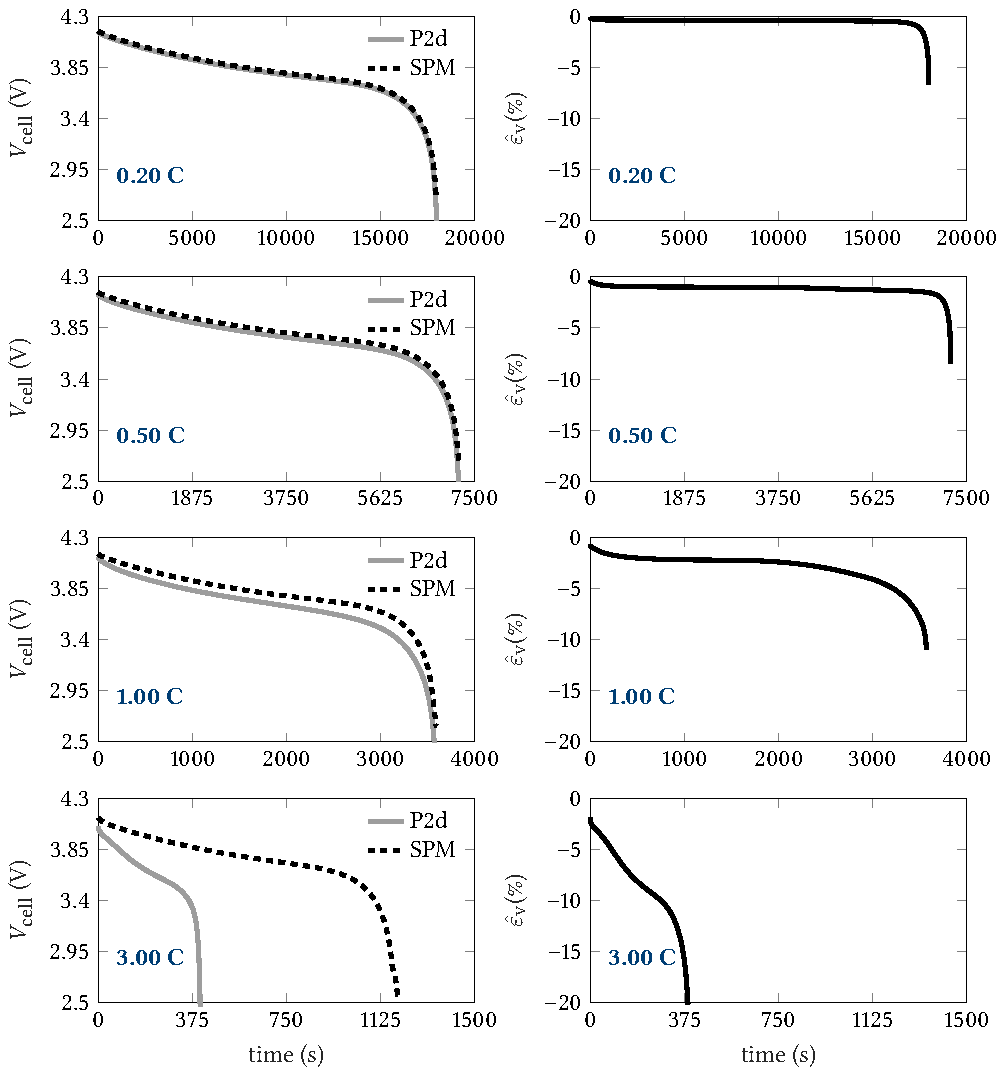
\includegraphics[width=\textwidth]{const_curr_dischg_voltage.pdf}
    \caption[Voltage responses of \glsfmtshort{p2d} and \glsfmtshort{spm} to
    constant current discharge]{Voltage responses of the \glsfmtshort{p2d} and
        \glsfmtshort{spm} models to various constant discharge rates. The left
        column shows the time-domain voltage response of the \gls{spm}
        plotted against the benchmark \glsfmtshort{p2d} response. The column on the
        right shows the percentage voltage error of the \glsfmtshort{spm} with
        respect to the \glsfmtshort{p2d} model. The performance of the
        \glsfmtshort{spm} degrades considerably at discharge currents above just~0.5C.}
    \label{fig:cnstdischgspmp2dvoltage}
\end{figure}

Since these comparisons  have to be done across multiple  C-rates, each yielding
different magnitudes in voltage responses, it is helpful to use a relative error
metric such as the percentage error, defined as
\begin{equation}
    \hat{\varepsilon}_v\,(\si{\percent}) = 100\frac{V_{\text{cell}_\text{p2d}} - V_{\text{cell}_\text{spm}}}{V_{\text{cell}_\text{p2d}}}
\end{equation}

It is to be noted that, in all cases, the \gls{p2d} model terminates faster than
the \gls{spm} either due to hitting lower cut-offs of either terminal voltage or
\gls{soc} (see \cref{fig:cnstdischgspmp2dsoc}).  Consequently, the  error vector
is defined only for the common time-region before cut-off.

In  \cref{fig:cnstdischgspmp2dvoltage},  the  column  on  the  right  shows  the
percentage error  in the voltage response  of the \gls{spm} with  respect to the
\gls{p2d} model.  At very  low C-rates  below \approx0.5C,  the voltage-response
performance of the \gls{spm} is acceptable. However, the performance degradation
is rapid above this C-rate. It is clear that the error in the \gls{spm} response
is monotonic and unidirectional. This indicates  that the source of the error is
due  to  unmodelled dynamics.  In  particular,  as  discussed in  the  modelling
assumptions  of  \cref{subsec:basicspmassumptions},  the \gls{spm}  ignores  the
electrolyte  dynamics.  Thus,  the  overpotential  in  the  electrolyte  is  not
modelled, which  results in the terminal  voltage of the \gls{spm}  being always
higher than its \gls{p2d} counterpart.

\begin{figure}[!htb]
    \centering
    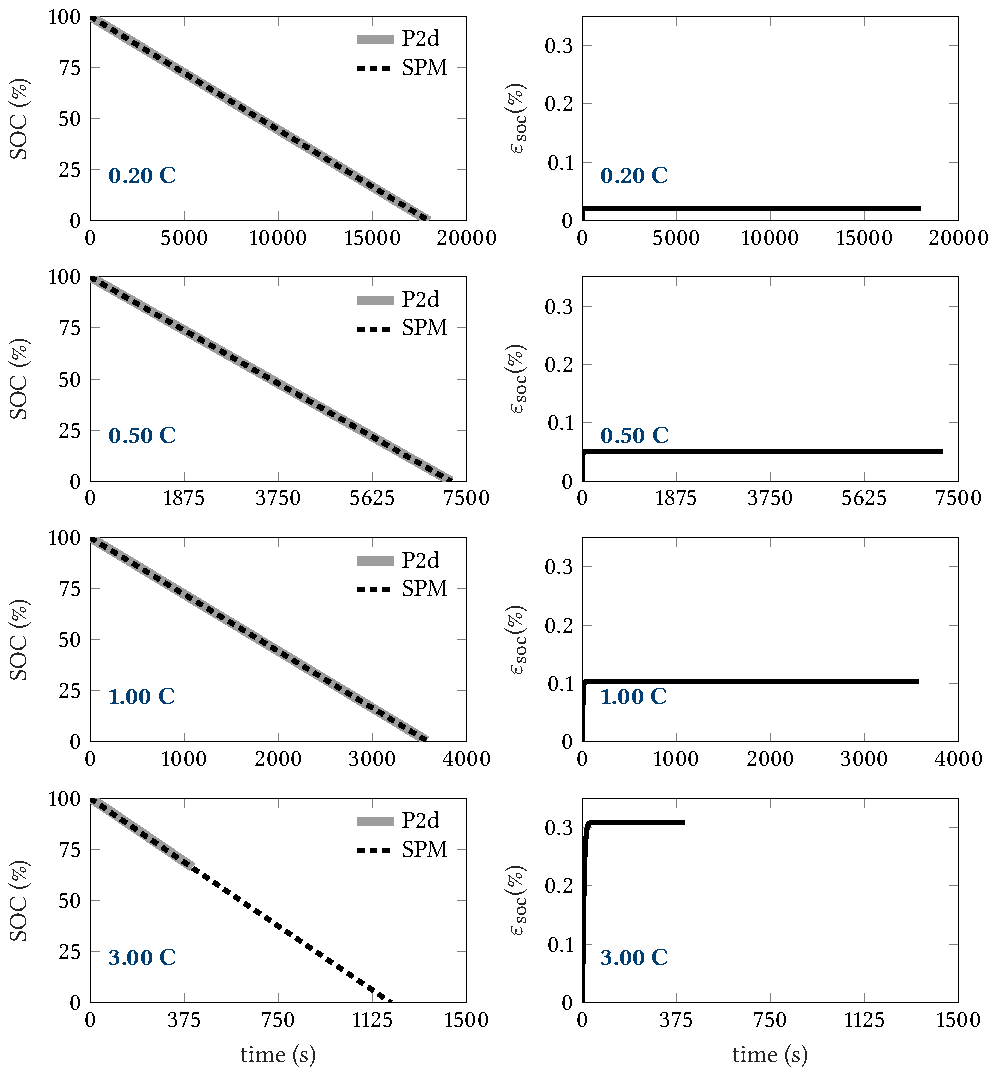
\includegraphics[width=\textwidth]{const_curr_dischg_soc.pdf}
    \caption[\glsfmtshort{soc} computed by \glsfmtshort{p2d} and
    \glsfmtshort{spm} models for constant current discharge]{Plots in the left
        column depict the time evolution of \glsfmtshort{soc} computed by the
        \glsfmtshort{p2d} and \glsfmtshort{spm} models for various constant
        discharge rates. The column on the right shows the error of the
        \glsfmtshort{soc} computed by the \glsfmtshort{spm} with respect to that
        computed by the \glsfmtshort{p2d} model \ie~$ \varepsilon_\text{soc}
        = {z_\text{p2d}} - z_\text{spm} $. The \glsfmtshort{spm} remains quite
    accurate even at moderate currents such as~3C.}
    \label{fig:cnstdischgspmp2dsoc}
\end{figure}

\Cref{fig:cnstdischgspmp2dsoc}  shows  the  time-evolution  of~\glsfmtshort{soc}
computed by the  \glsfmtshort{p2d} and the \glsfmtshort{spm}  models for various
discharge  currents. Since  the  \gls{soc} of  a cell  is  already a  normalised
quantity by  definition, the difference between  the two models can  be directly
used for comparison across C-rates. The \gls{soc} error is defined as
\begin{equation}
    \varepsilon_\text{soc} = {z_\text{p2d}} - z_\text{spm}
\end{equation}
and   like  the   error  in   the  terminal   voltage,  remains   unidirectional
over  time,   and  defined  only   until  one   of  the  models   hits  cut-off.
\Cref{tbl:errorsummarycntcurrdischgspmp2d}  shows  a  summary of  various  error
metrics used  to quantify  the performance  of the  basic \gls{spm}  for various
discharge rates.

% -*- root: ../../main.tex -*-
%!TEX root = ../../main.tex
% this file is called up by main.tex
% content in this file will be fed into the main document
% vim:nospell

\begin{table}[!htbp]
    \caption[Error-metrics summary of basic \glsfmtshort{spm} for constant current discharge]{Summary of error metrics
    of the basic \glsfmtshort{spm} for terminal voltage and \glsfmtshort{soc} in constant current discharge simulations.}
    \label{tbl:errorsummarycntcurrdischgspmp2d}
    \centering
    \begin{tabular}{@{} S S S S S @{}} \toprule
        {C-rate} & \multicolumn{2}{c}{$\hat{\varepsilon}_v\, (\si{\percent})$} & \multicolumn{2}{c}{$\varepsilon_\text{soc}\, (\si{\percent})$} \\
        \cmidrule(lr){2-3} \cmidrule(l){4-5}
        {}       & {abs.\ max.}                                                & \glsfmtshort{mae}                                               & {abs.\ max.} & \glsfmtshort{mae} \\ \midrule
        0.2      & 6.64                                                        & 0.49                                                            & 0.02        & 0.02        \\
        0.5      & 8.49                                                        & 1.17                                                            & 0.05        & 0.05        \\
        1.0      & 11.00                                                       & 2.95                                                            & 0.10        & 0.10        \\
        3.0      & 56.53                                                       & 9.22                                                            & 0.31        & 0.30        \\ \bottomrule
    \end{tabular}
\end{table}


A   quick   perusal  of \cref{tbl:errorsummarycntcurrdischgspmp2d}   reveals   a
discrepancy that invokes surprise at first glance. Whilst the performance of the
\gls{spm} is  quite poor in  terms of terminal  voltage prediction, it  is worth
noting that its \gls{soc} prediction  capabilities remain quite accurate even at
moderate  discharge  currents  of  about~3C and  therefore,  warrants  a  brief
explanation.

Referring to \cref{eq:soccomputation}, it is  seen that the \glsfmtshort{soc} of
the cell  is directly proportional  to the  bulk (average) concentration  in the
negative  electrode.  Hence  the plots  of  \cref{fig:cnstdischgspmp2dsoc}  also
represent the solid  phase concentration with a constant scaling  factor. As per
the assumptions listed in  \cref{subsec:basicspmassumptions}, the only transport
phenomena  modelled in  the \gls{spm}  is  solid phase  diffusion. However,  for
computation of the terminal  voltage, the electrolyte overpotential contribution
has  been  omitted  (see  \cref{eq:posoverpotential,eq:negoverpotential}).  This
explains  why  the  voltage  accuracy suffers,  while  the  open-loop  \gls{soc}
computation  remains  accurate.  The  high accuracy  of  \gls{soc}  (and  hence,
solid-phase  concentration)   computation  also  validates  the   usage  of  the
\engordnumber{4} order polynomial  approximation in the place of  Fick's law for
modelling solid-phase diffusion.

However,  the  discrepancy  in  accuracies of  terminal  voltage  and  \gls{soc}
computed  by the  basic \gls{spm}  leads to  an important  implication. Even  at
moderate C-rates, the  basic \gls{spm} \emph{cannot} be effectively  used in the
design of \gls{soc}  observers. This is because, the measured  voltage maps to a
vastly different  operating point when using  the \gls{spm} as the  plant model,
leading to strong deviations of the estimated \gls{soc}.


\subsubsection*{Constant current charge}\label{subsubsec:cnstcurrchgsim}

The \gls{cccv} charging  profile is a widely adopted  standard charging strategy
for charging lithium ion cells~\cite{Andrea2010}. In the constant current phase,
a charging rate of~1C is used  as an accepted baseline, although faster charging
strategies are presently being actively sought after.

% both in academia and in  particular, the automotive industry. For establishing
% the charging  performance of the basic  \gls{spm}, the standard rate  of~1C is
% used.

\begin{figure}[!htbp]
    \centering
    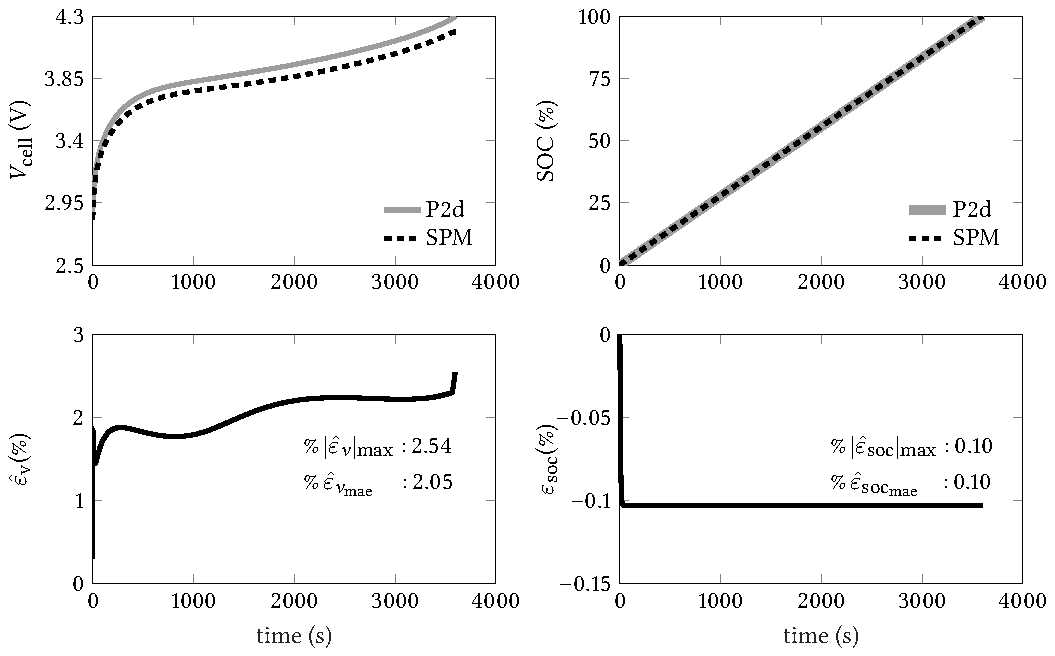
\includegraphics[width=\textwidth]{const_curr_chg.pdf}
    \caption[Voltage and \glsfmtshort{soc} computed by \glsfmtshort{p2d} and
    \glsfmtshort{spm} for 1C~constant current charge]{Time evolution of voltage
        and \glsfmtshort{soc} (top row) of the \glsfmtshort{p2d} and
        \glsfmtshort{spm} models upon charging with a constant current of~1C,
        \ie~\SI{60}{\ampere} starting at \SI{0}{\percent}~\glsfmtshort{soc}.
        The bottom row shows the percentage in terminal voltage and
        \glsfmtshort{soc} respectively of the \glsfmtshort{spm} with respect to
    the \glsfmtshort{p2d} model.}
    \label{fig:cnstchgspmp2d}
\end{figure}

The top row of \cref{fig:cnstchgspmp2d}  shows the evolution of terminal voltage
and \gls{soc}  of the \gls{p2d} and  \gls{spm} models under an  applied charging
current of~1C  \ie~\SI{60}{\ampere}. The constant-voltage charging  phase is not
shown. The bottom row shows the corresponding errors of the \gls{spm} model with
respect to  the reference  \gls{p2d} benchmark. The  corollary behaviour  of the
constant current discharge  behaviour is observed here. The  terminal voltage of
the \gls{spm}  remains below  the \gls{p2d} model  throughout. This  is expected
since, to  account for the  electrolyte voltage  drop modelled in  the \gls{p2d}
dynamics, a  higher terminal voltage needs  to be applied. The  voltage error is
thus  unidirectional and  remains positive  (opposite to  that observed  for the
corresponding  discharge  case). Similarly,  the  \gls{soc}  plots overlap  very
closely,  thereby validating  the underlying  polynomial approximation  of solid
phase diffusion.  It is  striking to  note that the  error in  \gls{soc} remains
exactly  around  the  same  magnitude (\approx\SI{0.1}{\percent})  in  both  the
charging and discharging cases.

\subsubsection*{Dynamic input profile}\label{subsubsec:dynamicspmp2dsim}

For automotive applications, it is  important to characterise the performance of
the  cell  model  under  dynamic load  conditions.  Several  standard  vehicular
driveycles  have been  defined and  adopted  by regulatory  agencies across  the
world.  These drivecycles  describe  the profile  of the  vehicle's  speed as  a
function of time.  The profile of speed versus time  of drivecycles is typically
available in intervals of \SI{1}{\second},  and is therefore consistent with the
sample interval used for the simulation (see \cref{tbl:lcoSimParamsSPMp2d}).

The \gls{udds} is  one such well-known drivecycle, originally  introduced by the
United  States  Environmental Protection  Agency  that  represents city  driving
conditions  which can  be  applied  to a  typical  mid-sized passenger  vehicle.
%  This  cycle  has  been  widely adopted  by  regulatory  agencies  across  the
world. \Cref{fig:uddsspeedvstimecycle}  shows the \gls{udds}  drivecycle wherein
the  vehicle's  speed  has  been  converted  to SI  units  for  use  in  further
computations.  One  complete  drivecycle runs  for~\SI{1369}{\second}.  As  seen
in  \cref{fig:uddsspeedvstimecycle}, the  \gls{udds} profile  is highly  dynamic
consisting  of  many sets  of  rapid  acceleration  and braking  events.  Hence,
this  drivecycle is  chosen to  provide  representative results  of the  model's
performance to dynamic inputs.

\begin{figure}[!htbp]
    \centering
    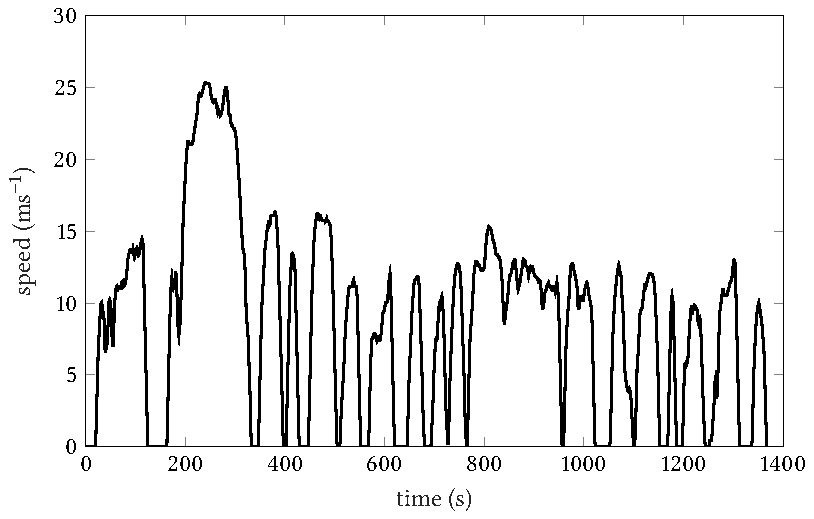
\includegraphics{udds_cycle.pdf}
    \caption{The \glsfmtshort{udds} drivecycle profile}
    \label{fig:uddsspeedvstimecycle}
\end{figure}

In  an  all-electric  drivetrain  wherein  lithium  ion  batteries  provide  the
propulsion power, the speed profile can be suitably converted to a corresponding
current  profile  experienced by  the  cell  through  the application  of  basic
governing   equations  from   vehicle   dynamics  (see   \cref{sec:accpathway}).
Therefore,  from  the  cell's  perspective, traversal  of  the  drivecycle  then
corresponds  to  the following  events.  During  acceleration phases,  the  cell
experiences  a  sharp  discharge  spike of  current.  Similarly,  assuming  that
regenerative  braking is  employed,  each deceleration  event  corresponds to  a
charging  current. Thus  a  current  versus time  dynamic  load  profile can  be
obtained. To  briefly summarise the  conversion process used here,  the computed
power profile of the cell is divided  by its nominal voltage and suitably scaled
so that the peak  of the current profile corresponds  to a discharge current
of~3C. Considering that all the braking energy cannot be recovered due to losses
at  the wheels,  brake discs  and  other mechanical  components, a  regenerative
braking  factor of  \SI{85}{\percent}  (the fraction  of  recoverable power)  is
assumed for  the charging scenario.

% The details  of this conversion for  a specific \gls{bev} platform  is discussed
% in~?\fxnote{fix this to point to layer opt chapter}.

\begin{figure}[!htbp]
    \centering
    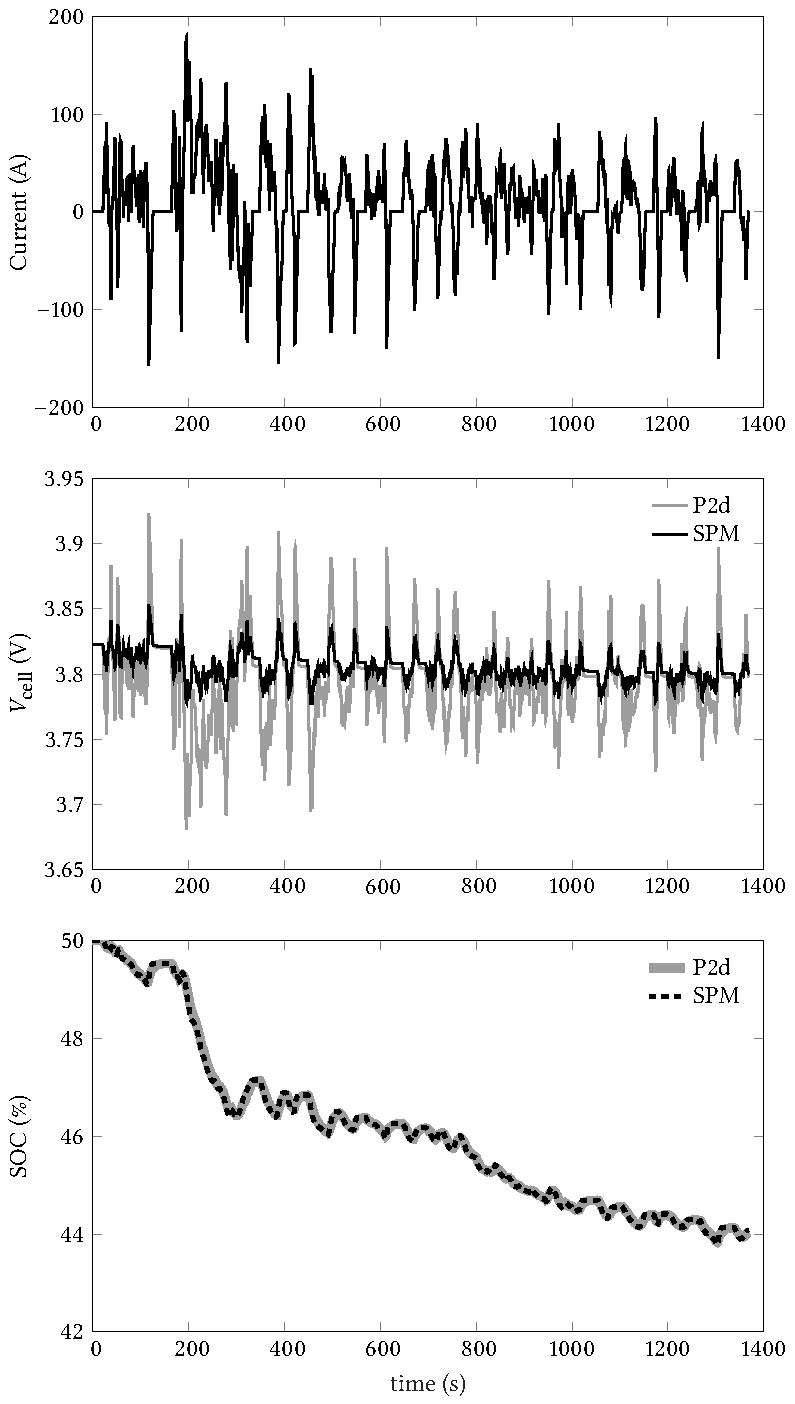
\includegraphics[width=10.890625cm]{udds_I_v_soc.pdf} % change the width suitably afterwards
    \caption[Simulation results of \glsfmtshort{p2d} and \glsfmtshort{spm}
    models to \glsfmtshort{udds} current profile]{Simulation results for a
        \glsfmtshort{udds} current profile. The voltage prediction performance
        of the \glsfmtshort{spm} to dynamic loads is poor while its
    \glsfmtshort{soc} computation accuracy is high.}
    \label{fig:uddssimp2dspmresults}
\end{figure}

\Cref{fig:uddssimp2dspmresults}  shows   the  simulation  results   obtained  by
applying   the   \gls{udds}   current   input  profile   (top   row)   to   both
the   \gls{p2d}   and  \gls{spm}   models.   The   simulation  is   started   at
\SI{50}{\percent}  cell~\gls{soc}. This  is representative  of the  median point
for  the  operating   window  of  \gls{soc}  swing  for   both  \glspl{bev}  and
\glspl{phev}~\cite{Maksimovic2012}. Although  regenerative braking  is employed,
due  to  the  reduced  occurrence  of braking  events  as  well  as  considering
efficiencies of  the drivetrain, as  with any driveycle, the  \gls{udds} profile
also results in a net-discharge. The  cell's \gls{soc} at the termination of the
\gls{udds} run is \approx\SI{6}{\percent} lower than its starting value.

% \FloatBarrier

The  voltage  output   from  the  models  is  plotted  in   the  middle  row  of
\cref{fig:uddssimp2dspmresults}.  The  bottom row  shows  the  evolution of  the
cell's \gls{soc}  over time. Consistent  with the  error trends observed  in the
constant current discharge and charge simulations, the error in terminal voltage
is  high whereas  that in  \gls{soc} is  low. In  this work,  the voltage  error
metrics  are reported  directly in  units  of \si{\milli\volt}  for the  dynamic
simulation run. Furthermore,  it is a standard practice to  report the \gls{rms}
error for such dynamic load profiles and is therefore included in the summary of
error metrics reported in \cref{tbl:errorsummaryuddsdischgspmp2d}.

% -*- root: ../../main.tex -*-
%!TEX root = ../../main.tex
% this file is called up by main.tex
% content in this file will be fed into the main document
% vim:nospell

\begin{table}[!htbp]
    \caption[Error-metrics summary of basic \glsfmtshort{spm} for \glsfmtshort{udds} current profile]{Summary of error
        metrics  of the basic \glsfmtshort{spm} with  \glsfmtshort{udds} input profile.}
    \label{tbl:errorsummaryuddsdischgspmp2d}
    \centering
    \begin{tabular}{@{} l S S @{}} \toprule
        {Error metric} & {$\varepsilon_v\, (\si{\milli\volt})$} & {$\varepsilon_\text{soc}\, (\si{\percent})$} \\ \midrule
        {Abs.\ max.}   & 97.37                                  & 0.21                                         \\
        {\gls{mae}}    & 19.38                                  & 0.04                                         \\
        {\gls{rms}}    & 25.88                                  & 0.06                                         \\ \bottomrule
    \end{tabular}
\end{table}


% accuracy comparison, figure inset

% textwidth in cm: \printinunitsof{cm}\prntlen{\textwidth} % 15.74776 cm
% textheight in cm: \printinunitsof{cm}\prntlen{\textheight} % 22.27184 cm
% github toolbox


% % Table comparing simulation speeds for cts and disc for constant current and dynamic current

% \section{Towards Enhancing the Conventional \glsfmtshort{spm}}\label{sec:electrolyteinclusion}
% % -*- root: ../../main.tex -*-
%!TEX root = ../../main.tex
% this file is called up by main.tex
% content in this file will be fed into the main document
% vim:textwidth=80 fo=cqt

As  evidenced by  the  results of  the constant  current  charge, discharge  and
dynamic  simulation runs,  the basic  \gls{spm} suffers  from a  \emph{critical}
drawback. The lack of electrolyte dynamics in the conventional \gls{spm} results
in poor  voltage accuracy  even at  moderate {C-rates}.  This renders  the model
unsuitable for  observer design in  \gls{soc} estimation applications  since the
output voltage from the model maps  to a radically different \gls{soc} operating
point. A number of candidate solutions have been proposed in literature in order
to mitigate this drawback. Their salient aspects are briefly evaluated here.

Even  the earliest  works which  attempt  to include  electrolyte dynamics  into
the  conventional  \gls{spm} were  published  only  within the  present  decade.
Schmidt~\etal~\cite{Schmidt2010c} proposed  an infinite-sum  eigenfunction modal
expansion paradigm for solving for the electrolyte concentration. It was claimed
that by  accounting for contribution from  only the first two  terms, sufficient
accuracy may be achieved. Furthermore, an \gls{ode} was proposed for the rate of
evolution of  the first temporal  mode. The solved electrolyte  concentration is
then  substituted into  an  approximate analytical  solution  for the  \gls{dfn}
model's  charge  conservation  \gls{pde} (see  \cref{eq:dfnliquidpotential})  to
obtain the electrolyte potential. However, the presentation lacks the sufficient
depth of explanation which hinders reproducibility. For instance, the origin and
explanation of the approximation terms  in the electrolyte potential solution is
omitted.  Derivations are  performed  from a  rigorous mathematical  perspective
without  providing contextual  reference to  cell parameters  or electrochemical
quantities. Introducing numerical examples would have been a redeeming factor to
help  keeping the  mathematical  aspects  tractable. This  method  has not  seen
further uptake for \gls{spm} modelling.

Guo~\etal~\cite{Guo2011a}  presented an  empirical approach  to account  for the
solution-phase dynamics.  Using standard curve-fitting techniques,  a non-linear
resistance as  a function of current  and temperature was introduced.  Thus, the
equation for cell terminal voltage presented
in \cref{eq:cellterminalvoltagebasic} is modified as
\begin{equation}
    V_\text{cell} = η_\text{pos} - η_\text{neg} + U_\text{pos} - U_\text{neg} - I R_\text{eq}
\end{equation}
where  $R_\text{eq}$~is  the  equivalent  resistance newly  introduced.  In  the
opinion of  this thesis  author, this  approach is too  simplistic and  does not
generalise well. Even if giving up  physics-based model origins can be tolerated
for one  or two subsystems  within the model,  the equivalent resistance  is not
just a minor correction term since it  needs to account for a large polarization
voltage of  the order  of tens of  millivolts. Secondly,  the current-dependence
introduced  to account  for the  complex mass  and charge  transport within  the
electrolyte  places a  disproportionately large  weight on  the accuracy  of the
curve-fitting process. Non-linear fits as proposed in Guo~\etal{} are inherently
problematic  in nature  as  the optimisation  routine may  converge  to a  local
minimum.  The  specific  form  and  nature \eg~the  convexity  of  the  proposed
hypothesis  function is  not  discussed.  It is  also  not  guaranteed that  the
same  fitting function  is  applicable  to a  different  cell  with another  set
of  parameters.  Finally, the  correction  term  being  resistive in  nature  is
zeroth order  \ie~cannot account  for the frequency  dependent behaviour  of the
electrolyte's  dynamics. This  approach is  more suited  for small-scale  static
corrections that do not  depend on the current \eg~to account for  a few tens of
microvolts due to a constant contact resistance of the current collectors.

% \fxnote{later on, as a capstone work, mention how I was inspired}

Di   Domenico~\etal{}~\cite{DiDomenico2010}  were   the  first   to  present   a
step-by-step  derivation   of  the   approximate  analytical  solution   to  the
electrolyte overpotential. The potential drop in the electrolyte is given by
\begin{equation}\label{eq:electrolytepd}
    \phi_\epos - \phi_\eneg = -\frac{I}{2 A}\left(\frac{l_\text{neg}}{\kappa_\text{eff}} + 2 \frac{l_\text{sep}}{\kappa_\text{eff}} + \frac{l_\text{pos}}{\kappa_\text{eff}}\right)
\end{equation}
and   can   be   substituted    into   the   subtraction   operation   involving
\cref{eq:posoverpotential}  and  \cref{eq:negoverpotential}   in  computing  the
overall  overpotential   of  \cref{eq:overpotentialdifference}  and   hence  the
terminal  voltage. The  effective conductivity  of  the electrolyte  in a  given
region  \jinpossepneg{},  within  the cell,  is  defined  as~${\kappa_\effj(c_e)
=    \kappa(c_e)\,    \varepsilon_j^{\text{brugg}_j}}$.    As    discussed    in
\cref{subsec:basicspmsimsetup},   the   intrinsic   and  hence   the   effective
electrolyte conductivity is a function of the concentration of \ch{Li^+} ions in
the  electrolyte.  Di  Domenico~\etal{}  did  not  discuss  the  spatio-temporal
calculation  of  electrolyte  concentration.  It   is  likely  that  a  constant
electrolyte  concentration  at  its  initial  equilibrium  value  was  used.  As
seen  in \cref{fig:ce1cdischgwithzoom},  significant  spatial  gradients in  the
electrolyte are established at even low  to moderate {C-rates} during the cell's
operation.  Sustained application  of  a unidirectional  current  even leads  to
starvation of ions in the electrolyte, particularly near the current collectors.
This  phenomenon  is  visualised in  \cref{fig:ce1cdischgwithzoom}  wherein  the
electrolyte  at the  positive current  collector is  virtually depleted  of ions
at  the  end  of  discharge.  This  ion-starvation  process  occurs  earlier  at
higher {C-rates}  and spreads throughout  the thickness of the  electrode. Thus,
the  assumption  of constant  ionic  concentration  in  the electrolyte  is  not
true.  Neglecting mass  transport due  to diffusion  implies that  the terms  in
\cref{eq:electrolytepd} constitute only  a part of the  expression for computing
the electrolyte  overpotential. Furthermore, Di Domenico~\etal{}  do not present
any results of  applying dynamic current profiles. Since the  critical aspect of
mass transport contribution to electrolyte  overpotential is omitted, this model
cannot be viewed as a \emph{sufficient} enhancement to the basic \gls{spm}.

\begin{figure}[!htbp]
    \centering
    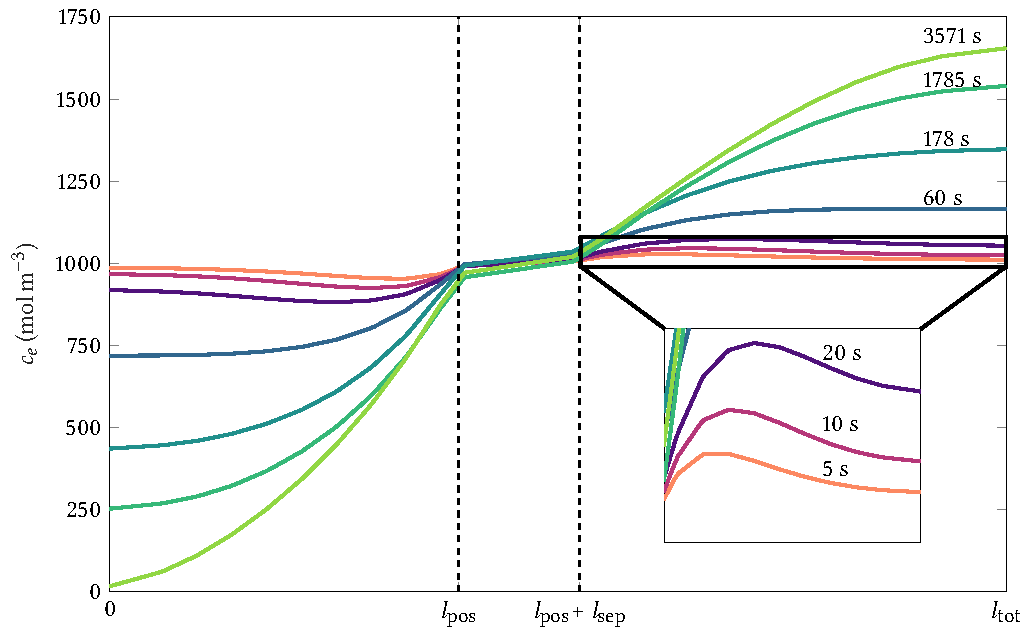
\includegraphics{ce_1C_at_various_times.pdf}
    \caption[Electrolyte conc.\ (time-snapshots) along cell thickness for 1C
    discharge]{\ch{Li^+} ion concentration in electrolyte along cell thickness
        at various time-snapshots during a 1C discharge simulation of the
        \glsfmtshort{p2d} model. A \glsfmtlong{qss} (\glsfmtshort{qss}) spatial
        profile  with inflection point at each separator interface begins to
        form at \approx \SI{60}{\second} after discharge begins. However, the
        ionic concentration in electrolyte exhibits a significantly different
        transient behaviour (zoomed inset) possessing another inflection point
        that disrupts the monotonic trend. Depletion of ionic concentration at
        positive current collector  towards end of discharge is also seen
    (bottom left).}
    \label{fig:ce1cdischgwithzoom}
\end{figure}

Although  not presented  in the  context  of incorporating  into the  \gls{spm},
Guduru~\etal~\cite{Guduru2012}   derived   an   analytical   solution   of   the
spatio-temporal  evolution  of  electrolyte concentration  using  the  \gls{sov}
method. The \gls{sov} method was first  applied to lithium ion cell modelling by
Subramanian~\etal~\cite{Subramanian2001a}  in order  to  solve  for solid  phase
concentration  profiles in  spherical  electrode particles.  Although the  ionic
concentration  in  the electrolyte  computed  by  the analytical  expression  in
Guduru~\etal{} seems like a feasible choice for inclusion into the \gls{spm}, it
is only applicable for galvanostatic  boundary conditions \ie~when the applied
current  is held  constant over  time. By  natural extension,  researchers could
hypothesise  that this  restriction  may  be removed  by  considering the  input
current as  piecewise constant  over small sample  intervals. Such  a hypothesis
could  be  reinforced  by  the  fact that  standard  drivecycles  are  specified
as  discrete  samples and  the  discrete-time  \gls{spm} processes  these  input
samples assuming \gls{zoh} behaviour. However, the analytical solution presented
in  Guduru~\etal{}  assumes  a  \gls{qss} concentration  profile.  The  authors'
presentation  considers a  near-instantaneous  establishment  of this  \gls{qss}
and  suggests a  parameter  independent analysis  through  use of  dimensionless
concentrations and time-constants instead of absolute time.

In  the  studies  conducted  by  this  thesis  author,  significantly  different
transient  behaviour  is exhibited  by  the  electrolyte concentration  profile.
Furthermore,  the  time  taken  to   establish  the  \gls{qss}  profile  is  not
negligible. This  difference in behaviour  could be attributed to  the different
parameter  set used.  \Cref{fig:ce1cdischgwithzoom}  shows  the spatial  profile
of  ionic concentration  at  various  snapshots of  time  during  a 1C  constant
current  discharge.  Starting  at \SI{100}{\percent}  \gls{soc},  the  discharge
lasts  \SI{3571}{\second}. It  is  seen that  it  takes nearly  \SI{60}{\second}
to  establish  the approximately  parabolic  shape  assumed by  the  electrolyte
concentration. After the initial transient has elapsed, the underlying structure
of the mathematical equations can be assumed  to be static. This is evidenced by
the  fact that  at  \SI{1785}{\second} \ie~after half  of  the discharge  is
completed, the shape of the curve is  nearly identical to the one towards end of
discharge. These  \gls{qss} curves  have their sole  inflection points  at their
separator  interfaces and  remains monotonic  within their  respective electrode
regions.  The  difference in  height  for  various  times  can be  accounted  by
the  coefficients  solved  using  the  analytical  modal  solution  proposed  in
Guduru~\etal{}.

The  axes  in  the  inset  of \cref{fig:ce1cdischgwithzoom}  shows  a  zoomed-in
view  of  the electrolyte  concentration  during  the transient  phase,  wherein
the  \gls{qss}  has  not  yet  been  established.  In  particular,  there  exist
additional inflection points,  one within the interior of  each electrode, which
renders the transient concentration profile mathematically incompatible with the
monotonicity  exhibited  by  the  \gls{qss} profile.  Thus,  in  highly  dynamic
operating  conditions with  frequent reversals  in  the direct  of current,  the
\gls{qss} assumption for the galvanostatic analytical solution becomes harder to
uphold without introducing significant  errors. Finally, the analytical solution
profile in Guduru~\etal{}  is not amenable to embedded  implementation, since it
consists of a non-trivial set of trigonometric computations at each time-step.

Prada~\etal~\cite{Prada2012} were  the first to provide  a simplified expression
for potential drop in the electrolyte  by including the terms representing ionic
concentration gradient within the cell thickness. Thus, \cref{eq:electrolytepd}
gets modified as
\begin{equation}\label{eq:electrolytepdwithce}
    \phi_\epos - \phi_\eneg = (1-t_{+}^0) \frac{2RT}{F}\ln \frac{c_\text{e,\tiny pos/cc}}{c_\text{e,\tiny neg/cc}}-\frac{I}{2 A}\left(\frac{l_\text{neg}}{\kappa_\text{eff,neg}} + 2 \frac{l_\text{sep}}{\kappa_\text{eff,sep}} + \frac{l_\text{pos}}{\kappa_\text{eff,pos}}\right)
\end{equation}
Although  the complete  expression for  electrolyte overpotential  was provided,
it   was  presented   in  a   cursory  manner \ie~without   detailing  the
spatio-temporal  computation  of  ionic  concentration  values  at  the  current
collector interfaces. Nevertheless, it is important to note this contribution as
\cref{eq:electrolytepdwithce} is widely relied upon by subsequent literature and
shall be used in \cref{sec:newelectrolytemodel}.

% in the original work of electrolyte concentration distributio presented by thisn
% thesis author i                                                                n


Rahimian~\etal{}~\cite{KhaleghiRahimian2013}   were   the   first   to   provide
approximate expressions for both charge  transport and mass transport properties
of the electrolyte specifically with the focus on improving the basic \gls{spm}.
The  authors discuss  the usage  of a  polynomial approximation  for electrolyte
concentration and potentials.  In particular, a cubic polynomial  was chosen for
approximating the  electrolyte concentration within the  porous electrodes. This
necessitates the  need to solve  for eight coefficients for  uniquely describing
the electrolyte concentration profile within  the electrode regions. However, in
the standard \gls{dfn} model, the number of electrolyte-specific \glspl{pde} and
their corresponding boundary conditions describing  charge and mass transport is
insufficient to uniquely  solve for all unknown coefficients  of this polynomial
approximation.  A detailed  explanation  of this  equation  deficiency shall  be
discussed in \cref{subsec:quadraticsimresultsanalysis}.

To overcome the issue of  equation deficiency, Rahimian~\etal{} adopted a scheme
wherein one  additional spatial location in  the interior of each  electrode was
also needed. The coefficients of the polynomial approximation were then obtained
by iteratively solving a large  coupled system of algebraic equations, embedding
within  them  the additional  equations  evaluated  at  the interior  points.  A
complicating issue  that arises  is regarding the  optimal positioning  of these
additional interior  points. An online  numerical optimisation was  performed to
obtain  the optimal  placement of  this interior  node. In  the opinion  of this
thesis author, these optimisation results could be sensitive to the thickness of
the electrodes  among other  parameters. A  discussion of  the stability  of the
proposed routine and its robustness to  parameter variance shall help in lending
confidence in the proposed method.  Although sufficient accuracy of the improved
\gls{spm} was  demonstrated for  currents up  to 5C, a  notable omission  is the
discussion of the model's performance  to dynamic input profiles. In conclusion,
the author of this thesis opines that, although this method serves as a proof of
concept towards implementing polynomial approximations for electrolyte dynamics,
until the aforementioned  gaps are addressed with clarity, it  is not convincing
for uptake by relevant stakeholders.

Kemper  and  Kum~\cite{Kemper2013} presented  an  approach  wherein the  spatial
gradients  of the  electrolyte concentration  are neglected.  The time-evolution
of  \emph{average}  ionic  concentration  in  each of  the  three  cell  regions
\viz~positive electrode,  separator and  negative electrode  are described  by a
set  of three  \glspl{ode}.  As  established by  the  discussion  thus far,  the
concentration gradients  along the axial  thickness of the cell  is significant,
even at  moderate {C-rates}.  Lending strength  to doubts  on the  model's wider
applicability  is the  fact that  results  from constant  current inputs  (which
induce large concentration  gradients in electrolyte) have not  been reported in
this work. Thus,  this approach is deemed as not  satisfactory enough to warrant
further engagement.

Luo~\etal~\cite{Luo2013} derived  a parabolic  approximation of  the electrolyte
concentration  distribution along  the  thickness of  the  cell. The  derivation
is  obtained  for  the case  of  steady-state  wherein  the  rate of  change  of
concentration  is  zero.  However,  the  author  of  this  thesis  is  sceptical
about  this since  in  the simulations  performed there  is  no situation  other
than  prior to  application of  current that  this exact  steady-state condition
is  satisfied.  In  the  \gls{qss}   profile  concept  discussion  based  on  on
\cref{fig:ce1cdischgwithzoom}, it is clear  that only the \emph{spatial} profile
reaches a shape that can be  potentially described by a mathematically invariant
family of curves. The electrolyte concentration is still \emph{time-varying} and
therefore violates the static time-evolution assumption. Although Luo~\etal{} do
not explicitly acknowledge this, they provide an extension for general operating
conditions  by introducing  exponential scaling  functions~$f_n(t)$ and~$f_p(t)$
while retaining the  assumption of parabolic spatial  behaviour. The computation
of certain time-constants in these scaling functions are not elucidated nor is a
summary  of procedural  steps for  determination of  the aforementioned  scaling
functions provided.


In a subsequent paper by  the same authors \ie~Luo~\etal~\cite{Luo2013a}, the
electrolyte concentration  model together  with a  similarly-derived electrolyte
potential model  was incorporated into  the conventional \gls{spm} to  arrive at
what the authors term as extended \gls{spm}. In this work, the electrolyte
potential is set to account for contribution from two terms ---
\begin{enumerate*}[label=\emph{\alph*})]
    \item ohmic drop due to bulk solution resistance and
    \item polarization potential due to concentration gradients
\end{enumerate*}
Although it  seeks to correctly account  for the two causes  of overpotential in
the  electrolyte,  there  is  no  detailed explanation  on  the  computation  of
quantities such as time-constants involved in the polarization potential term.

A modified version of the electrolyte model proposed in Luo~\etal~\cite{Luo2013}
was  used  in Zou~\etal~\cite{Zou2016a}  for  observer  design in  an  \gls{soc}
estimation  application. The  modification  essentially  consists of  truncating
the complex  expression in~\cite{Luo2013}  consisting of  six coefficients~$p_1$
through~$p_6$ to just two, and elimination of the aforementioned time-constants.
However, to  the disappointment  of the  author of this  thesis, the  claim that
truncation to~$n=2$ terms is sufficient to  describe the dynamics proved  to be
optimistic for  the parameter set considered.  In my attempts to  reproduce this
work, an  arbitrary scaling  factor was  needed to  correct for  the electrolyte
potential drop  and match  the \gls{p2d} simulations.  The requirement  for such
scaling factors  whose physical  origins are not  clearly identifiable  lends to
scepticism on the model's robustness. Furthermore,  it was found that this value
needed to be  hand-tuned for each parameter-set. Until these  gaps are addressed
clearly, it is worth seeking other  viable alternatives to model the electrolyte
dynamics.

After  completing  the  simulations  with  the  aforementioned  scaling  factors
and  continuing  in  the  quest  for other  alternatives,  the  author  of  this
thesis  made  an observation  that  other  researchers  have  had to  resort  to
similar techniques  for describing the electrolyte  overpotential. For instance,
Han~\etal~\cite{Han2015a}  use a  similar  scaling factor~$p<0$  for the  entire
expression   of  \cref{eq:electrolytepdwithce}   representing  the   electrolyte
overpotential   using  the   polynomial  approximation   approach  proposed   by
Rahimian~\etal~\cite{KhaleghiRahimian2013}.  However, these  unexplained scaling
factors lower the confidence regarding the model's general applicability.


Tanim~\etal~\cite{Tanim2014}  accounted  for  electrolyte dynamics  by  deriving
reduced   order  transfer   functions  for   ionic  concentration   distribution
and   electrolyte  overpotential   using  the   \gls{ima}  technique.   However,
the  coefficients  of   these  transfer  functions  are   excessively  long  and
comprised  of   chained  algebraic   operations  expressed  in   a  high-entropy
sum-of-products  form  in  the  appendix   of  their  work.  For  instance,  ten
coefficients  are  needed  to  describe  the  concentration  profile  while  six
coefficients  are required  for  the electrolyte  potential.  The median  length
of  each  atomic  sub-expression  of these  coefficients  is  sufficiently  high
to  obfuscate   their  physical  significance.   A  low-entropy  form   for  the
coefficients  of  these   transfer  functions  similar  to   that  pioneered  by
Middlebrook~\cite{Middlebrook} and  exemplified in the  design-oriented analysis
of  electric   circuits~\cite{Middlebrook1998,Vorperian2002}  could   have  been
helpful to aid the readers' understanding.  The author of this thesis recognises
that  mathematical complexity  should  not be  the sole  basis  to evaluate  the
merits of  such proposed improvements.  Although the presentation of  these long
coefficients have been judiciously moved  to the appendix, their derivations ---
essential to prove the model's validity  --- is curiously omitted. The length of
the mathematical  expressions increases  the probabilities of  introducing human
errors during implementation.

It  is worth  noting that  Marcicki~\etal~\cite{Marcicki2013} had  independently
proposed a similar approach \viz~deriving a transcendental transfer function
from  electrolyte  concentration  to  applied  current, albeit  for  a  cell  of
\gls{lfp} chemistry. This transfer function  consisted of a series of hyperbolic
trigonometric functions which  were later truncated by  Padé approximation (see
\cref{subsec:freqdomainroms}  for  a  brief  introduction  to  frequency  domain
\glspl{rom}). However, upon trying this approach for the \gls{lco} parameter set
by this thesis'  author, in order to obtain sufficient  accuracy, the truncation
order had  to be  raised to  at least seven,  similar in  complexity to  that of
Tanim~\etal~\cite{Tanim2014a}.  In  both Marcicki~\etal~\cite{Marcicki2013}  and
Tanim~\etal~\cite{Tanim2014a},  the  electrolyte-specific  enhancements  to  the
\gls{spm} are in  the frequency domain, placing further  burden, particularly on
industry stakeholders to accurately interpret  and transform the coefficients to
a time-domain implementation  for deployment in an embedded  \gls{bms}. Owing to
this,  as  already  stated in \cref{subsec:freqdomainroms},  these  models  fall
outside the scope of this thesis.
% ignoring prof plett's latest work on electrolyte transfer functions

Fan~\etal~\cite{Fan2016}   proposed   an   Extended  \gls{spm}   that   includes
electrolyte dynamics using  the \gls{gpm} which achieves  an acceptable accuracy
in terminal voltage  performance. Although the authors claim  that the \gls{spm}
is computationally  \emph{cheaper} than  other model order  reduction techniques
such as proper orthogonal decomposition  and balanced truncation, this claim has
not  been substantiated.  The sole  comparison of  CPU times  presented in  this
work  only compares  against  the classical  \gls{fdm}.  Although an  impressive
computational  speed is  achieved, it  is unclear  whether the  model equations,
particularly  those  involving  solutions  of  non-linear  integral  expressions
resulting from  applying the Galerkin's  method can  be solved in  real-time for
embedded implementation.  In the review of  this method conducted by  the author
of  this thesis,  it  appears  that the  Galerkin's  projection  method is  more
suitable  for  desktop  simulations.  In  congruence  with  my  scepticism,  the
authors  of~\cite{Fan2016} have  not claimed  the suitability  of this  work for
online/embedded  application  in a  \gls{bms}.  Therefore,  as per  this  thesis
authors' stance  explained in \cref{sec:classificationscheme},  models employing
such methods are deemed to be not in alignment with the goals of this thesis.

Moura~\etal~\cite{Moura2017} proposed an improved \gls{spm} by simply augmenting
the  conventional  \gls{spm}  with  a simplified  form  of  electrolyte-specific
equations of  the original  \gls{dfn} model. The  resulting model  therefore has
\glspl{pde} in it and therefore not easily amenable for embedded implementation.
Lotfi~\etal~\cite{Lotfi2017}  presented  an   algebraic  approximation  for  the
spatial  distribution   of  electrolyte  concentration  by   modifying  standard
parabolic expressions with leading exponential  coefficients. There are two main
issues with this approach. It is not explained why this mathematical formulation
was chosen  and its superiority  with respect to other  family of curves  is not
discussed. Secondly, these coefficients are to be determined through solution of
equations obtained by applying continuity  and flux boundary conditions from the
\gls{dfn}  model  for  electrolyte  concentrations  at  the  electrode-separator
interfaces. Since exponential-type expressions are assumed, the resulting set of
equations are non-linear,  the solving of which, especially in  the context of a
resource-constrained environment is problematic.

% The other main contribution of this work is its feasibility analysis of having
% convergent  estimators for  this model  and design  of such  a \gls{pde}-based
% estimator.  In  the  views of  this  thesis  author,  this  approach is  on  a
% trajectory that deviates  too far from a simplified model  suitable for online
% implementation.

In  the  authors'   observations  in  trying  to  replicate   the  results  from
the  literature  presented here,  the  errors  in  all such  approximations  can
be  attributed  to  inaccuracies  in  computing  the  spatio-temporal  evolution
of  electrolyte   concentration.  Upon   obtaining  a   good  estimate   of  the
electrolyte concentration profile, \cref{eq:electrolytepdwithce} is deemed to be
satisfactory for  the electrolyte  overpotential computation. Thus  attention is
focussed on solving for the electrolyte concentration profile.

From the discussion of literature, it is clear that the proposed enhancements to
the  computing the  ionic concentration  in electrolyte  falls into  one of  the
following two categories
\begin{itemize}
    \item model description through physical principles followed by mathematical
        simplification
    \item fitting of pre-assumed simplified mathematical structures to some
        physical phenomena
\end{itemize}

In the  views of the  author, it appears that  using the former  approach yields
technically  correct, yet  mathematically convoluted  expressions overpotentials
that are fraught with implementation  difficulties. Although the latter approach
looks  promising  in   terms  of  ease  of   implementation,  their  sub-optimal
performance and lack of wider-applicability leaves much to be desired. Among the
latter  class of  models, owing  to  its simplicity,  the quadratic  (parabolic)
approximation method for  electrolyte concentration is an  attractive option. It
is therefore  important to understand  the source  of weakness of  this specific
sub-class of  models. Such  an analysis  has not  been performed  in literature.
Hence,  the  author's  analysis  on   the  quadratic  approximation  method  for
electrolyte concentration is presented next in \cref{sec:quadraticapprox}.


% May also mention some typographical errors in Lotfi etal second paper
% Mention that parabolic profile is a common theme
% perhaps it cannot be done, but we do not give up. Equation deficiency

% But I  did something different. The high accuracy  of the \gls{soc}
% in  the  basic  \gls{spm}  leads  to  the  author's  hypothesis  that  if  the
% electrolyte  concentration  can be  solved  as  an independent  subsystem  and
% incorporated into the terminal voltage, this can lead to an improved \gls{spm}
% with electrolyte  dynamics. Such  a decoupled  electrolyte inclusion  into the
% basic \gls{spm}\fxnote{fix this sentence}



% \section{Quadratic Approximation of Ionic Spatial Concentration}\label{sec:quadraticapprox}
% % -*- root: ../../main.tex -*-
%!TEX root = ../../main.tex
% this file is called up by main.tex
% content in this file will be fed into the main document
% vim:textwidth=80 fo=cqt

As  evidenced by  the  results from  constant  current  charge, discharge  and
dynamic  simulation runs presented in \cref{sec:basicspmsimresults},  the basic 
\gls{spm} suffers  from poor voltage accuracy. The prior art discussed in
\cref{sec:electrolyteinclusion} aim to tackle this issue through inclusion of
electrolyte dynamics using various state of the art methods. However, they lack
in providing an in-depth analysis and expository illustration of the fundamental
deficiency of the standard \gls{p2d} dynamics, which is uncovered later in
\cref{subsec:symbolicreg}. This is facilitated through the introduction of the
quadratic approximation model of ionic spatial concentration in this
section\footnote{The  mathematical derivations  here  represents  the  author's 
    digested  summary  of  literature, and  is  particularly  based  upon  a 
portion  of  Deng~\etal~\cite{Deng2018}}. The quadratic approximation model is
notable since it serves as the baseline reference for inclusion of electrolyte
dynamics into an \gls{spm}.

% The  steps  involved  in  deriving   the  quadratic  approximation  is  detailed
% in  \cref{subsec:quadraticmodelderiv}.  Based  on   the  results  from  applying
% this   quadratic   approximation   scheme,   an   analysis   of   the   weakness
% of  this   model  is  performed   in  \cref{subsec:quadraticsimresultsanalysis}.

% Mitigation  of   this  critical  drawback   lead  to  this   author's  decoupled
% spatio-temporal electrolyte concentration model  structure which is presented in
% \cref{sec:newelectrolytemodel}.

\subsection{Model derivation}\label{subsec:quadraticmodelderiv}

The  schematic  in  \cref{fig:coordsquadapprox}  shows  the  definition  of  the
co-ordinate  systems  used  in  deriving the  polynomial  approximation  of  the
electrolyte  concentration   profile.  The  three   regions~${\{\text{neg,  sep,
pos}\}}$  are  abbreviated  to ${\{n,s,p\}}$~respectively  in  all  mathematical
expressions. The globally defined $x$~co-ordinate starts at the negative current
collector interface~(${x=0}$)  and terminates at the  positive current collector
interface  ($x  = l_\text{tot},\,  \text{where  }  l_\text{tot} =  l_\text{n}  +
l_\text{s} + l_\text{p}$). Three local co-ordinate systems~$z$ valid only within
their respective regions are also defined.  In particular, it must be noted that
the direction of  the local $z_\text{pos}$~co-ordinate axis is  opposite to that
of the other two local co-ordinate axes as well as the global co-ordinate axis.

% In subsequent usages, the  suffix in~$z_\mu$  is dropped  and  the  reader is  advised  to infer  the region  of  validity from  the  usage  context  which  are unambiguous  as  they occur  in separate  equations.

% The author is  convinced that this notation  does not
% detract  from following  the  derivations, but  rather aids  it  by keeping  the
% notations compact.

\begin{figure}[!htbp]
    \captionsetup{singlelinecheck=off}
    \centering
    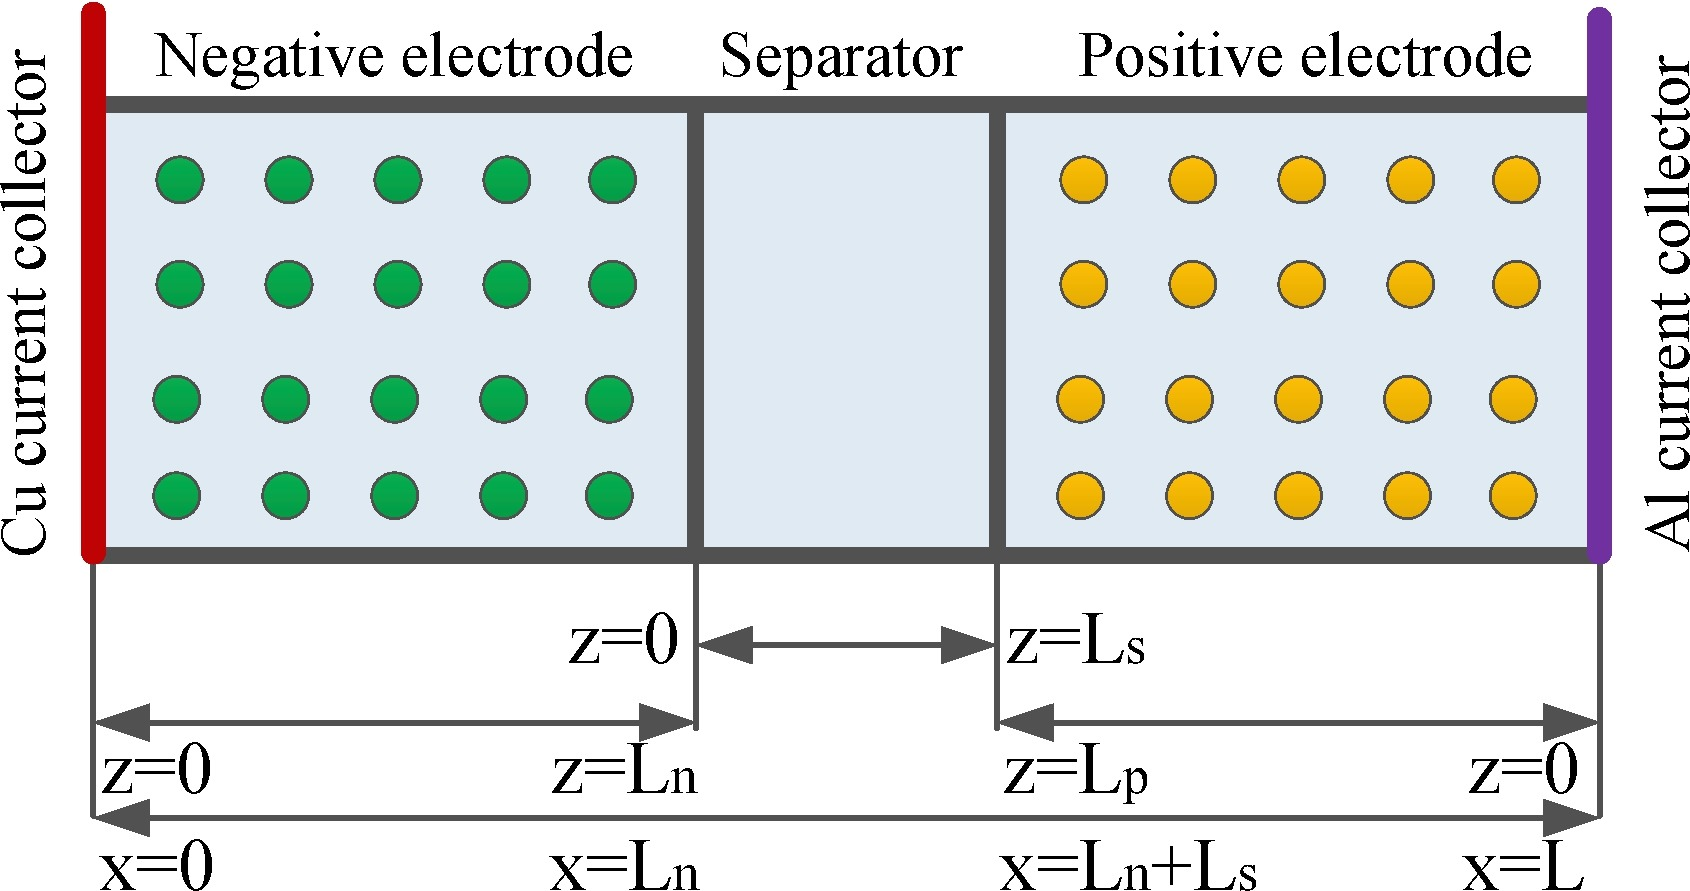
\includegraphics{co_ord_sys}
    \caption[Co-ordinate systems for quadratic approximation of
    electrolyte concentration]{Schematic diagram of the electrochemical sandwich
        consisting of
        \begin{enumerate*}[label=\itshape\alph*\upshape)]
            \item negative electrode,
            \item separator, and
            \item positive electrode
        \end{enumerate*} depicting the co-ordinate system used in deriving the
        quadratic approximation profile. The global spatial co-ordinate is~${x
            \in \{0,L\}}$, where~${L = l_\text{tot} = l_\text{neg} + l_\text{sep} +
        l_\text{pos}}$. Local co-ordinate systems~$z$ specific to each
        region are also defined. It should be noted that the positive
        electrode's local co-ordinate axis direction is reversed with respect to
        the global co-ordinate axis. Illustration reproduced from
    Deng~\etal~\cite{Deng2018}.}
    \label{fig:coordsquadapprox}
\end{figure}

A  standard  quadratic  expression  is chosen  a~priori  for  approximating  the
electrolyte  concentration  profile  within each  region.
\begin{alignat}{2}  %
    % \SwapAboveDisplaySkip
   c_\ensub(z,t) & = a_2(t) z^2  + a_1(t) z + a_0(t) \qquad     &  & 0 \le z \le l_\text{n}\label{eq:cenqquadstart} \\
   c_\essub(z,t) & = a_5(t) z^2 + a_4(t) z + a_3(t) \qquad      &  & 0 \le z \le l_\text{s}\label{eq:cesqquadstart} \\
   c_\epsub(z,t) & =  a_8(t) z^2  + a_7(t)  z  + a_6(t)  \qquad &  & 0  \le z  \le l_\text{p}\label{eq:cepqquadstart}
\end{alignat}
The time-dependent coefficient  vector ${\vec{a}(t) = \vect{a_0(t),a_1(t),
\dots ,a_8(t)}}$ is to be determined\footnotemark.
\footnotetext{Hereafter, the  explicit  time-dependence  of  the
coefficients  is  omitted.  Similarly,  the  spatio-temporal
dependence of the electrolyte  concentration~$c_{\text{e,}j}$ is also dropped
from the notation.}
Applying     boundary     conditions     of    the     electrolyte     diffusion
equation   from   the   \gls{dfn}   model~(refer   \cref{eq:dfnliquiddiff})   to
\crefrange{eq:cenqquadstart}{eq:cepqquadstart},  it is  clear that  ${a_1 =  0}$
and~${a_7 = 0}$. Thus, \crefrange{eq:cenqquadstart}{eq:cepqquadstart} become
\begin{alignat}{2}
    % \SwapAboveDisplaySkip
    c_\ensub      & = a_2 z^2 + a_0         \qquad          &  & 0 \le z \le l_\text{n}\label{eq:cenquadreduced} \\
    c_\essub      & = a_5 z^2 + a_4 z + a_3 \qquad          &  & 0 \le z \le l_\text{s}\label{eq:cesquadreduced} \\
    c_\epsub      & = a_8 z^2 + a_6         \qquad          &  & 0 \le z \le l_\text{p}\label{eq:cepquadreduced}
\end{alignat}
with  the  coefficient  vector being  modified  to~${\vec{a} = \vect{a_0,a_2, \dots ,a_6, a_8}}$.


\Cref{tbl:dfnelectrolyteeqnsinsep} lists  the equations and  boundary conditions
for phenomena  describing electrolyte  diffusion and  charge balance  within the
separator domain.

% -*- root: ../main.tex -*-
%!TEX root = ../main.tex
% this file is called up by main.tex
% content in this file will be fed into the main document
% vim:nospell textwidth=180 foldlevelstart=3 foldlevel=3 conceallevel=0

\begin{table}[!htbp]
    \centering
    \caption[Electrolyte equations \& boundary conditions of \glsfmtshort{dfn} model in separator]{Electrolyte-specific governing equations and boundary conditions of the \glsfmtlong{dfn}~(\glsfmtshort{dfn}) model within the separator domain.}
    \label{tbl:dfnelectrolyteeqnsinsep}
    \begingroup
    \makeatletter\def\f@size{9.25}\check@mathfonts
    \addtolength{\jot}{0.875em}
    \begin{tabular*}{\textwidth}{@{} l c r l r @{}}
        \toprule
        \multicolumn{1}{c}{\small Region} & \small Governing equations & \multicolumn{2}{c}{\small Boundary conditions } & {} \\
        {} & {} & \multicolumn{2}{c}{\scriptsize $(l_\text{neg} \coloneqq l_\text{n},\, l_\text{sep} \coloneqq l_\text{s},\, l_\text{pos} \coloneq l_\text{p})$} \\
        \midrule
        \multicolumn{1}{l |}{{\rotatebox[origin=c]{90}{\makecell{\footnotesize Separator\\ \scriptsize $\delta \in \{\text{sep}\}$}}}} &
        $\begin{aligned}
            \vphantom{D_{\text{\tiny eff}_\text{n}}\!\! \! \!\, \diffp{c_\text{e}}{x}{\mathrlap{x = l^{-}_\text{n}}}} \varepsilon_\delta \diffp{c_\text{e}}{t} &=D_\effdelta  \diffp[2]{c_\text{e}}{x} \\[-0.75em]
            \vphantom{D_{\text{\tiny eff}_\text{s}}\!\! \! \!\, \diffp{c_\text{e}}{x}{\mathrlap{x=(l_{\text{n}} + l_\text{s})^{-}}}}\\[1.25em]
            \vphantom{\kappa_{\text{\tiny eff}_\text{n}}\!\! \! \!\, \diffp{c_\text{e}}{x}{\mathrlap{x = l^{-}_\text{n}}}\hspace{5mm} =\kappa_{\text{\tiny eff}_\text{s}}\!\!\!\!\,\diffp{c_\text{e}}{x}{\mathrlap{x = l^{+}_\text{n}}}} \frac{I}{A} &= \overline{\kappa}_\effdelta \left( \diffp[2]{\phi_\text{e}}{x} + \frac{2 R T}{F} (t^0_{+}-1)\diffp[2]{ \ln c_\text{e}}{x}\right) \\[-0.75em]
            \vphantom{\kappa_{\text{\tiny eff}_\text{s}}\!\! \! \!\, \diffp{c_\text{e}}{x}{\mathrlap{x=(l_{\text{n}} + l_\text{s})^{-}}}} \\
        \end{aligned}$ &
        $\begin{aligned}
    \vphantom{D_{\text{\tiny eff}_\text{n}}\!\! \! \!\, \diffp{c_\text{e}}{x}{\mathrlap{x = l^{-}_\text{n}}}} \qquad c_\text{e}\Bigr\rvert_{\mathrlap{x=l^{-}_\text{n}}}\hspace{5mm} &= c_\text{e}\Bigr\rvert_{\mathrlap{x=l^{+}_\text{n}}},\\[-0.75em]
     \vphantom{\kappa_{\text{\tiny eff}_\text{n}}\!\! \! \!\, \diffp{c_\text{e}}{x}{\mathrlap{x = l^{-}_\text{n}}}\hspace{5mm} =\kappa_{\text{\tiny eff}_\text{s}}\!\!\!\!\,\diffp{c_\text{e}}{x}{\mathrlap{x = l^{+}_\text{n}}}} c_\text{e}\Bigr\rvert_{\mathrlap{x=(l_{\text{n}} + l_\text{s})^{-}}}\hspace{5mm} &= c_\text{e}\Bigr\rvert_{\mathrlap{x=(l_{\text{n}} + l_\text{s})^{+}}},\\[1.25em]
 \vphantom{\kappa_{\text{\tiny eff}_\text{n}}\!\! \! \!\, \diffp{c_\text{e}}{x}{\mathrlap{x = l^{-}_\text{n}}}} \vphantom{\left( \diffp[2]{\phi_\text{e}}{x} + \frac{2 R T}{F} (t^0_{+}-1)\diffp[2]{ \ln c_\text{e}}{x}\right)} \phi_\text{e}\Bigr\rvert_{\mathrlap{x=l^{-}_\text{n}}}\hspace{5mm} &= \phi_\text{e}\Bigr\rvert_{\mathrlap{x=l^{+}_\text{n}}},\\[-0.75em]
 \vphantom{\kappa_{\text{\tiny eff}_\text{s}}\!\! \! \!\, \diffp{c_\text{e}}{x}{\mathrlap{x=(l_{\text{n}} + l_\text{s})^{-}}}} \phi_\text{e}\Bigr\rvert_{\mathrlap{x=(l_{\text{n}} + l_\text{s})^{-}}}\hspace{5mm} &= \phi_\text{e}\Bigr\rvert_{\mathrlap{x=(l_{\text{n}} + l_\text{s})^{-}}},\\
    \end{aligned}$ &
    $\begin{aligned}
        \quad D_{\text{\tiny eff}_\text{n}}\!\! \! \!\, \diffp{c_\text{e}}{x}{\mathrlap{x = l^{-}_\text{n}}}\hspace{5mm} &=D_{\text{\tiny eff}_\text{s}}\!\!\!\!\,\diffp{c_\text{e}}{x}{\mathrlap{x = l^{+}_\text{n}}}\\[-0.75em]
        D_{\text{\tiny eff}_\text{s}}\!\! \! \!\, \diffp{c_\text{e}}{x}{\mathrlap{x=(l_{\text{n}} + l_\text{s})^{-}}}\hspace{5mm} &=D_{\text{\tiny eff}_\text{p}}\!\!\!\!\,\diffp{c_\text{e}}{x}{\mathrlap{x=(l_{\text{n}} + l_\text{s})^{+}}}\\[1.25em]
        \vphantom{\left( \diffp[2]{\phi_\text{e}}{x} + \frac{2 R T}{F} (t^0_{+}-1)\diffp[2]{ \ln c_\text{e}}{x}\right)} \kappa_{\text{\tiny eff}_\text{n}}\!\! \! \!\, \diffp{c_\text{e}}{x}{\mathrlap{x = l^{-}_\text{n}}}\hspace{5mm} &=\kappa_{\text{\tiny eff}_\text{s}}\!\!\!\!\,\diffp{c_\text{e}}{x}{\mathrlap{x = l^{+}_\text{n}}}\\[-0.75em]
        \kappa_{\text{\tiny eff}_\text{s}}\!\! \! \!\, \diffp{c_\text{e}}{x}{\mathrlap{x=(l_{\text{n}} + l_\text{s})^{-}}}\hspace{5mm} &=\kappa_{\text{\tiny eff}_\text{p}}\!\!\!\!\,\diffp{c_\text{e}}{x}{\mathrlap{x=(l_{\text{n}} + l_\text{s})^{+}}}\\
    \end{aligned}$ &
    $\begin{aligned}
        \vphantom{D_{\text{\tiny eff}_\text{n}}\!\! \! \!\, \diffp{c_\text{e}}{x}{\mathrlap{x = l^{-}_\text{n}}}} \quad \refstepcounter{equation}(\theequation)\label{eq:liquiddiffnsep} \\[-0.75em]
        \vphantom{D_{\text{\tiny eff}_\text{s}}\!\! \! \!\, \diffp{c_\text{e}}{x}{\mathrlap{x=(l_{\text{n}} + l_\text{s})^{-}}}}\\[1.25em]
        \vphantom{\kappa_{\text{\tiny eff}_\text{n}}\!\! \! \!\, \diffp{c_\text{e}}{x}{\mathrlap{x = l^{-}_\text{n}}}} \vphantom{\left( \diffp[2]{\phi_\text{e}}{x} + \frac{2 R T}{F} (t^0_{+}-1)\diffp[2]{ \ln c_\text{e}}{x}\right)} \refstepcounter{equation}(\theequation) \label{eq:liquidpotentialsep}\\[-0.75em]
        \vphantom{\kappa_{\text{\tiny eff}_\text{s}}\!\! \! \!\, \diffp{c_\text{e}}{x}{\mathrlap{x=(l_{\text{n}} + l_\text{s})^{-}}}}
    \end{aligned}$
    \\
    \bottomrule
\end{tabular*}
\endgroup
\end{table}



\Cref{eq:liquiddiffnsep}  and   \cref{eq:liquidpotentialsep}  are   obtained  by
applying   the  pertinent   electrolyte   equations  of   the  \gls{dfn}   model
(\cref{eq:dfnliquiddiff} and  \cref{eq:dfnliquidpotential} respectively)  to the
separator  region. Applying  the continuity  and flux  boundary conditions  from
\cref{eq:liquiddiffnsep} at both separator interfaces,
\begin{alignat}{2}
    \SwapAboveDisplaySkip
    \allowdisplaybreaks
    a_2 l^2_\text{n} + a_0                      & = \hphantom{-}a_3 \qquad                    &  & \text{\footnotesize (continuity at neg/sep interface)} \label{eq:cecontinuitynegsep} \\
    a_5 l^2_\text{s} + a_4 l_\text{s} + a_3     & = \hphantom{-}a_8 l^2_\text{p} + a_6 \qquad &  & \text{\footnotesize (continuity at sep/pos interface)}                               \\
    2 a_2 l_\text{n} D_\effn                    & = \hphantom{-}a_4 D_\effs \qquad            &  & \text{\footnotesize (flux b.c.\ at neg/sep interface)}                               \\
    \left(2 a_5 l_\text{s} + a_4\right) D_\effs & = -2 a_8 l_\text{p} D_\effp \qquad          &  & \text{\footnotesize (flux b.c.\ at sep/pos interface)}\label{eq:quadcefluxseppos}
\end{alignat}
The negative sign in \cref{eq:quadcefluxseppos} is due to the specific
choice of  the co-ordinate system  used for  the positive electrode  region (see
\cref{fig:coordsquadapprox}).  Due to  this,  fluxes  at the  separator/positive
electrode interface have opposing directions.
Let  $Q_\text{e,j}$  denote  the  number  of moles  of  \ch{Li^+}~ions  in  the
electrolyte per  unit cross-sectional  area within each  region~$\jinnegseppos$.
This is  computed as  the product  of
\begin{enumerate*}[label=\emph{\alph*})]
    \item the porosity and
    \item spatial integral of the concentration function
\end{enumerate*}
\ie~${ Q_\text{e,j}  =  \varepsilon_j \int_0^{l_j}  c_{\text{e},j}(z) \,dz  }$.
Applying this to \crefrange{eq:cenquadreduced}{eq:cepquadreduced}
\begin{align}
    Q_\text{e,n} &= \varepsilon_\text{n} \left( \frac{1}{3} a_2 l^3_\text{n} + a_0 l_\text{n}\right)\label{eq:Qenbyintegration}\\
    Q_\text{e,s} &= \varepsilon_\text{s} \left( \frac{1}{3} a_5 l^3_\text{s} + \frac{1}{2} a_4 l^2_\text{s} + a_3 l_\text{s}\right)\\
    Q_\text{e,p} &= \varepsilon_\text{p} \left( \frac{1}{3} a_8 l^3_\text{p} + a_6 l_\text{p}\right) \label{eq:Qepbyintegration}
\end{align}

\addlines
At this stage,  $Q_{\text{e},j}(t)$~are unknown. Since  these are time-dependent
functions,  the  derivation  naturally  progresses  towards  seeking  a  set  of
\glspl{ode} that describe a relationship  for their time evolution. Transforming
the  \engordnumber{2}   order  \glspl{ode}  of \cref{eq:dfnliquiddiff}   (for  electrodes)
and \cref{eq:liquiddiffnsep}   (for  separator)   to   their  respective   local
co-ordinates and integrate  once along the thickness of  each region. Performing
this sequence of steps for the negative electrode region
\mathleft
\begin{equation}
    \begin{WithArrows}[b]
        \varepsilon_\text{n} \int_0^{l_\text{n}} \left(\diffp*{c_\ensub(z,t)}{t}\right)\, dz &= \int_0^{l_\text{n}} \left(\diffp{}{z}\left(D_\effn \diffp{c_\ensub}{z} \right) + (1 - t^0_\text{+}) a_\snsub j_\text{n}\right)\, dz \Arrow[tikz={text width=3.4cm}]{transposing integration \& differentiation operations in the \glsfmtshort{lhs}} \\
        \varepsilon_\text{n} \diffp*{\int_0^{l_\text{n}} c_\ensub(z,t)}{t}\, dz &=
        \int_0^{l_\text{n}} \left(\diffp{}{z}\left(D_\effn \diffp{c_\ensub}{z}
        \right) + (1 - t^0_\text{+}) a_\snsub j_\text{n}\right)\, dz
        \Arrow[tikz={text width=3.4cm}]{apply time-derivative operator to the whole \glsfmtshort{lhs}}\\
        \diffp*{\left(\tikzmark{StartBraceA}\varepsilon_\text{n} \int_0^{l_\text{n}}
c_\ensub(z,t)\, dz\tikzmark{EndBraceA}\right)}{t} &=  \int_0^{l_\text{n}}
\left(\diffp{}{z}\left(D_\effn \diffp{c_\ensub}{z} \right) + (1 -
    t^0_\text{+}) a_\snsub j_\text{n}\right)\, dz \Arrow[tikz={text
width=3.4cm}]{apply integral to the \glsfmtshort{rhs}}\\
        \diff*{Q_\text{e,n}(t)}{t} &= D_\effn \diffp{c_\ensub}{z}{\mathrlap{z=l_\text{n}}} + (1 - t^0_\text{+}) a_\snsub \int_0^{l_\text{n}} j_\text{n}\, dz
    \end{WithArrows}
    \label{eq:negliionmolestoreduce}
\end{equation}
\mathcenter
\InsertUnderBrace[draw=black][aspect=0.26]{StartBraceA}{EndBraceA}{} % https://tex.stackexchange.com/questions/68526/asymmetric-overbrace
% \blindtext
% \AddToShipoutPicture*{\ShowFramePicture}
Performing     the     identical     sequence     of     operations     starting
from~(\cref{eq:liquiddiffnsep}) for  the separator and~(\cref{eq:dfnliquiddiff})
for the positive electrode yields
\begin{align}
    % \SwapAboveDisplaySkip
    \diff*{Q_\text{e,s}(t)}{t} &= D_\effs \diffp{c_\essub}{z}{\mathrlap{z=l_\text{s}}} \label{eq:sepliionmolestoreduce}\\
    \diff*{Q_\text{e,p}(t)}{t} &= D_\effp \diffp{c_\epsub}{z}{\mathrlap{z=l_\text{p}}} + (1 - t^0_\text{+}) a_\spsub \int_0^{l_\text{p}} j_\text{p}\, dz\label{eq:posliionmolestoreduce}
\end{align}

In    order    to   evaluate    the    integral    term   in    the    \gls{rhs}
of \cref{eq:negliionmolestoreduce}    and \cref{eq:posliionmolestoreduce},   the
solid  phase  charge  conservation  equation~(\cref{eq:solidchargeconserve})  is
integrated  along the  local  co-ordinate  axis of  the  negative electrode  and
positive electrode respectively.
\begin{align}
    \int_0^{l_\text{n}} j_\text{n}\, dz & =  \frac{I}{a_\snsub A F} \label{eq:negfluxintegral}\\
    \int_0^{l_\text{p}} j_\text{p}\, dz & =  \frac{-I}{a_\spsub A F}\label{eq:posfluxintegral}
\end{align}

Substituting       \crefrange{eq:negfluxintegral}{eq:posfluxintegral}       into
\crefrange{eq:negliionmolestoreduce}{eq:posliionmolestoreduce} respectively,
\begin{align}
    \allowdisplaybreaks
    \diff*{Q_\text{e,s}}{t} &= D_\effn \diffp{c_\ensub}{z}{\mathrlap{z=l_\text{n}}} - (1 - t^0_\text{+}) \cancel{a_\snsub} \frac{I}{\cancel{a_\snsub} A F} \\
    \diff*{Q_\text{e,p}}{t} &= D_\effp \diffp{c_\epsub}{z}{\mathrlap{z=l_\text{p}}} - (1 - t^0_\text{+}) \cancel{a_\spsub} \frac{-I}{\cancel{a_\spsub} A F}
\end{align}
which leads to the general expressions  for the cross-sectional molar density of
\ch{Li^+}~ions in each of the three regions as
\begin{align}
    \diff*{Q_\text{e,n}}{t} & = D_\effn \diffp{c_\ensub}{z}{\mathrlap{z=l_\text{n}}} + (1 - t^0_\text{+}) \frac{I}{A F} \label{eq:negliionmolesgen} \\
    \diff*{Q_\text{e,s}}{t} & = D_\effs \diffp{c_\essub}{z}{\mathrlap{z=l_\text{s}}} \label{eq:sepliionmolesgen}                                             \\
    \diff*{Q_\text{e,p}}{t} & = D_\effp \diffp{c_\epsub}{z}{\mathrlap{z=l_\text{p}}} - (1 - t^0_\text{+}) \frac{I}{A F}\label{eq:posliionmolesgen}
    \intertext{Substituting the assumed quadratic expressions for electrolyte concentrations in
        each of the three regions \crefrange{eq:cenquadreduced}{eq:cepquadreduced}
    in the above system \ie~\crefrange{eq:negliionmolesgen}{eq:posliionmolesgen}}
    \diff*{Q_\text{e,n}}{t} & = 2 a_2 l_\text{n} D_\effn + (1 - t^0_\text{+}) \frac{I}{A F} \label{eq:negliionmolesquadratic}                                \\
    \diff*{Q_\text{e,s}}{t} & = 2 a_5 l_\text{s} D_\effs\label{eq:sepliionmolesquadratic}                                                                                                     \\
    \diff*{Q_\text{e,p}}{t} & = 2 a_8 l_\text{p} D_\effp - (1 - t^0_\text{+}) \frac{I}{A F} \label{eq:posliionmolesquadratic}
\end{align}
\addlines
The  initial   ionic  concentration   in  the   electrolyte  is   identical  in
all  three  regions  of  the  cell,  assuming  equilibrium  starting  conditions
\ie~${c_{\text{e,0}_j}  = c_\text{e,0},  \jinnsp}$.  Hence the  initial number  of
moles of \ch{Li^+} per unit area in each of the three regions is given by
\begin{align}
    Q_\text{e,n}(0) & = \varepsilon_\text{n} c_\text{e,0} l_\text{n} \label{eq:Qeninit}\\
    Q_\text{e,s}(0) & = \varepsilon_\text{s} c_\text{e,0} l_\text{s}\\
    Q_\text{e,p}(0) & = \varepsilon_\text{p} c_\text{e,0} l_\text{p} \label{eq:Qepinit}\\
    \intertext{and the initial coefficient vector which satisfies the system
    equations is obtained as}
    \begin{bmatrix}
        a_0 \\
        a_2 \\
        a_3 \\
        a_4 \\
        a_5 \\
        a_6 \\
        a_8
        \end{bmatrix} & = \begin{bmatrix}
        c_\text{e,0} \\
        0 \\
        c_\text{e,0} \\
        0 \\
        0 \\
        c_\text{e,0} \\
        0
    \end{bmatrix} \label{eq:coeffinit}
\end{align}

The             system             of             three             \glspl{ode},
\eqref{eq:negliionmolesquadratic}--\eqref{eq:posliionmolesquadratic}    together
with  \crefrange{eq:Qeninit}{eq:Qepinit}  representing the  initial  conditions,
form   an    \gls{ivp}.   \Crefrange{eq:cecontinuitynegsep}{eq:Qepbyintegration}
represent a square system of seven linear algebraic equations with seven unknown
coefficients which must be solved at each time-step. These algebraic constraints
coupled with the aforementioned \gls{ivp} form a \gls{dae} system.

There are now two choices for proceeding  with solution of the system. The naive
approach  would be  to  solve  the \gls{dae}  using  advanced \gls{dae}  solvers
specially designed to handle \mbox{index-1}  semi-explicit systems such as
DASSL~\cite{Petzolddassl}
and  DASPK~\cite{VanKeken1995}. For  start-stop  type  of input  currents  with discontinuities,  the
consistent initialisation of algebraic conditions and derivatives is numerically
challenging.  All   \gls{dae}  solvers  typically  use   adaptive  time-stepping
algorithms.  The  feasibility of  using  such  a  complex scheme  for  real-time
computation is questionable. On the other hand, the overall system can be viewed
as composed of two numerical subsystems ---
\begin{enumerate*}[label=\emph{\alph*})]
    \item an independent \gls{ode} system, and
    \item an independent algebraic system.
\end{enumerate*}
Each system  is executed  back to  back in succession  using solutions  from the
other system from the previous time-step.

To  clarify  the sequence  of  operations,  in  order  to bootstrap  the  model,
it  is  required  to  compute  $Q_{\text{e},j}(t)$ in  all  three  regions.  The
\gls{ode} system is  integrated for one time-step by  retaining the coefficients
at  their initial  value.  The $Q_{\text{e},j}(t)$  thus  solved is  substituted
into  the  algebraic system  to  yield  the  updated  value of  the  coefficient
vector~$\vec{a}(t=t_k)$. This new value of the coefficient vector is substituted
back  into  the  \gls{ode}  system  and  the  process  continues.  Although  the
continuous simulation of  the overall \gls{dae} is not accomplished,  this scheme is
pragmatic from an engineering viewpoint. This is because,  the periodic pauses needed to update
the intertwined  sub-systems translate  naturally into  fixed time-steps  and is
well-suited for a \gls{bms} controller operating at a fixed sample rate. This is
also an effective workaround to mitigate the complexities of having to implement
and solve \glspl{dae} in real time.

% need to write algorithm
The   simulation   results   of   the   quadratic   approximation   scheme   and
the   analysis   of   its   strengths   and   weaknesses   is   presented   next
in \cref{subsec:quadraticsimresultsanalysis}.

\subsection{Numerical implementation, simulation results and analysis}\label{subsec:quadraticsimresultsanalysis}

\subsubsection*{Numerical implementation}
From an analysis point of view,  the quadratic approximation model for computing
the  spatio-temporal evolution  of  electrolyte concentration  can be  simulated
as  an  independent subsystem,  and  hence  can  be implemented  numerically  as
a  standalone  module as  shown  in  \cref{alg:quadraticce}. In  practice,  this
modular code  is embedded as  a subroutine within  the main \gls{spm}  loop (see
\cref{alg:disctimespm}).

% -*- root: ../main.tex -*-
%!TEX root = ../main.tex
% this file is called up by main.tex
% content in this file will be fed into the main document
% vim:nospell

\begin{algorithm}[!htbp]
    \caption{Quadratic approximation model for spatio-temporal electrolyte concentration}\label{alg:quadraticce}
    \begin{algorithmic}[1]
        \Require Load profile \Comment{\eg~a \texttt{csv} file of $t$ vs.\ C-rate}
        \Require Electrolyte model parameter set  \Comment{\eg~stored in a struct \texttt{ceparams}}
        \Userdata $ t_\text{f}$,  sample rate $T_s, c_\text{e,init}$
        \Function{QuadraticElectrolyteModel}{}
        \State Set $Q_{\text{e,init}_j}$ as per \crefrange{eq:Qeninit}{eq:Qepinit}
        \State $\vec{a}[1]$ \gets values from \cref{eq:coeffinit}
        \State $V_\text{cell}[1] \gets \textsc{ComputeCellVoltage}(\textbf{x}[1],I[1],\texttt{params})$ \Comment{from direct feedthrough}
        \For{$k \gets 2 : N_\text{max}$}
        \State $I[k] \gets $ interpolate from profile using \gls{zoh}
        \State Solve continuous-time state equations--\crefrange{eq:negliionmolesquadratic}{eq:posliionmolesquadratic} \Comment{Using $\vec{a}[k-1]$}
        \State $Q_{\text{e}_j}[k]$ \gets last time-entry  vector of soln.\  matrix \Comment{if using an adaptive solver}
        \State $\vec{a}[k]$ \gets solution of \emph{linear} system of equations--\crefrange{eq:cecontinuitynegsep}{eq:Qepbyintegration} \Comment{Using $Q_{\text{e}_j}[k-1]$}
        \State Compute $c_{\text{e}_j}$ as per \crefrange{eq:cenquadreduced}{eq:cepquadreduced} \Comment{Quadratic polynomial expressions for concentration}
        \EndFor
        \EndFunction
    \end{algorithmic}
\end{algorithm}


\begin{figure}[!htb]
    \centering
    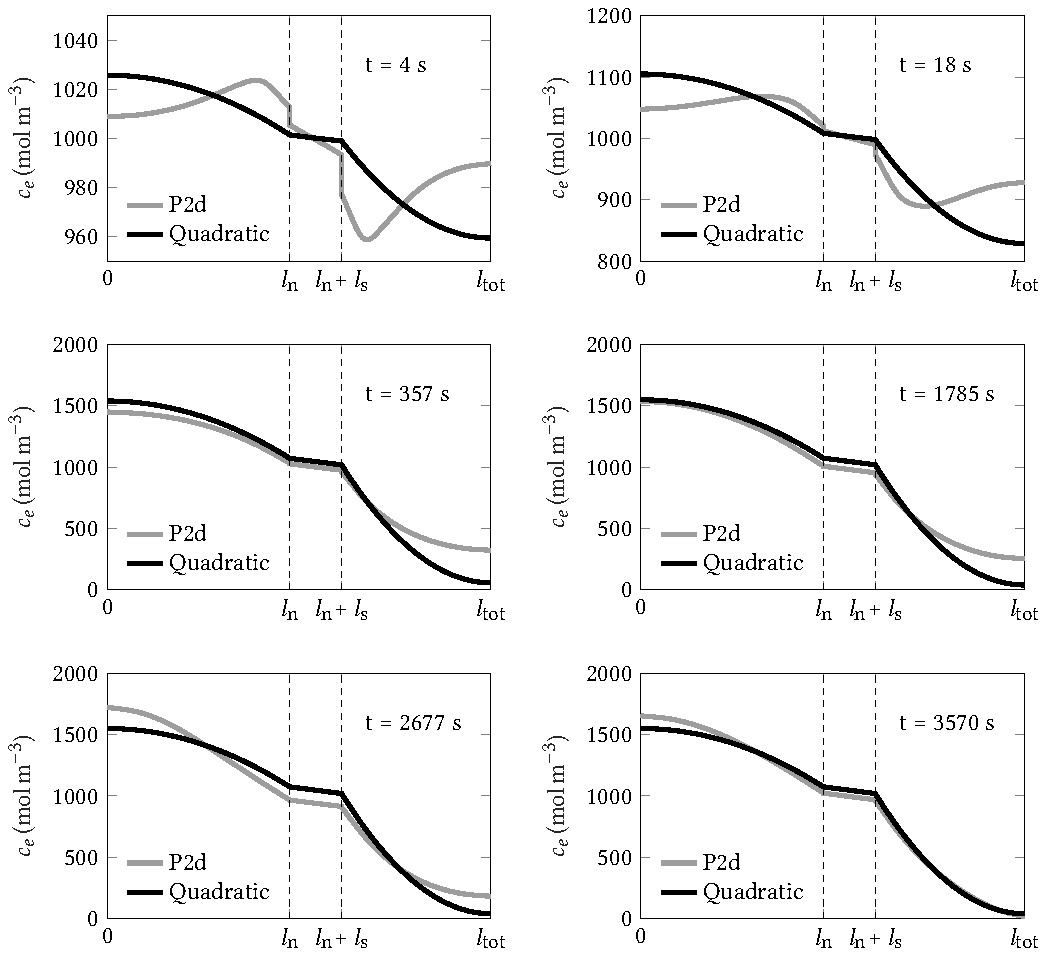
\includegraphics[width=\textwidth]{quadratic_ce_approx_spatial_1C.pdf}
    \caption[Spatial distribution of electrolyte concentration for 1C~discharge]{Spatial distribution of ionic concentration in electrolyte along
        cell thickness at various snapshots of time for a 1C~discharge. The
        concentration profile obtained from simulating the \glsfmtshort{p2d}
        model is used as the reference. The performance of the quadratic model
        is quite poor during the initial transient duration, but improves over
    time as a quasi-steady state is reached.}
    \label{fig:spatialionicconc1C}
\end{figure}


\subsubsection*{Simulation results}\label{subsubsec:simresultsbaselinequad}

\Cref{fig:spatialionicconc1C} shows  the spatial distribution of  \ch{Li^+}~ions
in electrolyte  along the  thickness of  the cell at  various snapshots  of time
obtained by simulation  of the \gls{p2d} and the  quadratic approximation models
using a  1C~discharge current. The  \gls{p2d} model's response is  considered as
the reference benchmark.  During the initial transient  phase, the concentration
profile within each electrode region exhibits a characteristic inflection point.
During this phase,  the concentration profile computed by  the parabolic profile
exhibits  a  large deviation  in  terms  of  percentage  error at  each  spatial
location. However, with the passage of time, as a \gls{qss}~is established, this
inflection point flattens out, and the quadratic approximation becomes closer to
the  true  concentration value  at  each  spatial  location. Similar  trends  in
behaviour is  exhibited for discharge and  charging at higher C-rates  and these
results are  therefore omitted here  in the  interest of keeping  the discussion
succinct.

It  is important  to  note that  while having  a  spatial concentration  profile
is  useful,  as  seen  in \cref{eq:electrolytepdwithce}, it  is  the  values  of
concentration  at   the  \emph{current  collector  interfaces}   that  are  most
influential in  computation of the  electrolyte overpotential and hence,  in the
voltage accuracy of the enhanced \gls{spm}. Thus, it is important to obtain this
alternative perspective  of time-evolution  of the electrolyte  concentration at
the two current collectors.

\begin{figure}[!htbp]
    \centering
    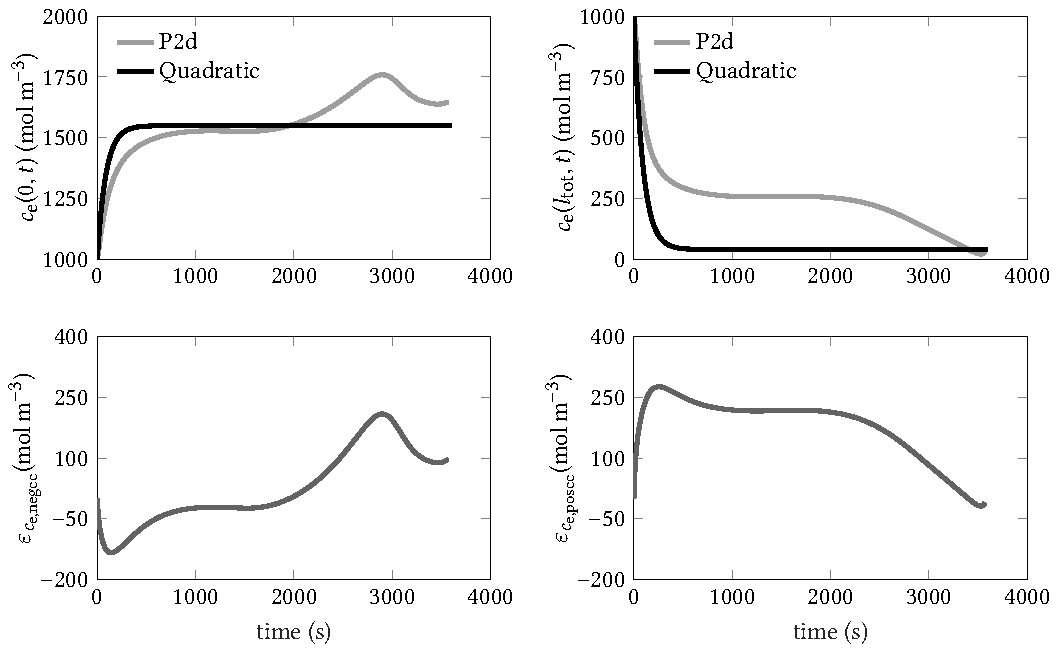
\includegraphics[width=\textwidth]{ce_at_cc_1Cdischg.pdf}
    \caption[Ionic concentrations at current collector
    interfaces over time for 1C~discharge]{Evolution of ionic concentration over
        time at the two current collector interfaces for a 1C~discharge (top
        row). The time evolution of the corresponding error variables is 
    shown in the bottom row of plots.}
    \label{fig:temporalcequadratic}
\end{figure}

\Cref{fig:temporalcequadratic} shows  the time evolution of  ionic concentration
in  the electrolyte  at the  two current  collector interfaces  computed by  the
\gls{p2d} and  quadratic approximation  models for a  1C~discharge  current. The
concentration  values computed  by  the  \gls{p2d} model  is  considered as  the
reference benchmark. At the negative electrode--current collector interface, the
ionic  concentration  exhibits  a  few oscillations  of  small  amplitude  owing
to  the complex  interactions  of  the ionic  phase  with  the porous  electrode
and  the charge  transfer process  at the  electrode-electrolyte boundary.  The
concentration  evolution  predicted  by  the quadratic  approximation  model  is
rather  simplistic  and  is  unable to  capture  this  intricate  time-evolution
pattern.  This  is because  the  governing  equation predicting  time  evolution
of  concentration  in  the  quadratic  approximation  model  is  that  given  by
the  \emph{first-order}  \gls{ode} of \cref{eq:negliionmolesquadratic}  (with  a
proportional mapping from~$Q_\text{e,n}$ to~$c_\text{e}(0,t)$). Following system
theory, the step response  of a first order \gls{ode} is  that of an exponential
rise to a final settling value, which  is exactly the shape seen in the top-left
plot of \cref{fig:temporalcequadratic}.

The ionic  concentration evolution  at the positive  current collector  does not
exhibit major oscillations  and even has a subtle monotonicity  to its response.
However,  the  classical  first  order  response  predicated  by  the  quadratic
approximation model falls short of representing its complete dynamics. Errors of
similar  magnitude  are present  in  the  ionic  concentration at  both  current
collector  interfaces, with  a maximum  absolute error  of \approx\SI{250}{\mole
\per \meter  \cubed}.
% Similar trends are  exhibited in charging, with  a swapped response pattern observed at the two current collector interfaces.



